% Course notes for Numerical Methods, MATH3018 and MATH6141
% Updated from the MATH3018 and MATH6111 Numerical Methods notes.
% Original notes by Giampaolo d'Alessandro
% Updated by Ian Hawke
% Rewritten for new syllabus by Ian Hawke

\documentclass[a4paper,12pt]{report}

\usepackage{SULecturePhysics}
\usepackage{tabularx}
\usepackage[linktoc=all]{hyperref}
\usepackage{textcomp}

%\includeonly{Interpolation}

%%%%%%%%%%%%%%%%%%%%
% Particular theorems
%%%%%%%%%%%%%%%%%%%%
%\newtheorem*{ConvThm}{Convolution Theorem}
%\newcounter
\newtheorem{Properties}{Properties}

%%%%%%%%%%%%%%%%%%%%
% A general unnumbered theorem
%%%%%%%%%%%%%%%%%%%%

%\newtheorem*{thm}{Theorem}

%%%%%%%%%%%%%%%%%%%%
% Environments used as theorems....
%%%%%%%%%%%%%%%%%%%%
\newtheorem{corollary}{Corollary}[chapter]
\newtheorem{definition}{Definition}[chapter]
\newtheorem{Example}{Example}[chapter]
%\newtheorem{theorem}{Theorem}[chapter]
\newtheorem{lemma}{Lemma}[chapter]

\usepackage{color}

%%%%%%%%%%%%%%%%%%%%
% And here we go
%%%%%%%%%%%%%%%%%%%%

\begin{document}

%%%%%%%%%%%%%%%%%%%%
% Title page
%%%%%%%%%%%%%%%%%%%%

\title{MATH3018 \& MATH6141 \\ Numerical Methods }
\author{Dr.~Ian~Hawke\\ Content provided under a \\Creative Commons attribution license, CC-BY 4.0. \\ \textcopyright\ 2017 Ian Hawke.}
%\author{Dr.~Ian~Hawke}
\date{}

\maketitle

%%%%%%%%%%%%%%%%%%%%
% Table of Contents
%%%%%%%%%%%%%%%%%%%%

\begin{titlepage}
%\fancyhf{}
\newpage
\mbox{}
\end{titlepage}

\tableofcontents

\chapter{Error analysis}

\section{Introduction}

Numerical analysis is mathematics brought down to earth.  In the world
of mathematics   numbers   are exact:   $\pi$ is  the   ratio  of  the
circumference to its radius and it is known exactly, each single digit
after  the other.  Numerical analysis teaches  humbleness: it tells us
that in  the real world  we cannot know numbers  exactly, we  can only
know 2, 20, a million of the digits that form the number $\pi$, but in
no way we can know any non-rational number exactly.  This may not seem
a serious problem: does it really matter that we cannot represent more
than 10 of the  first digits of  $\pi$?   The answer to  this specific
question is that generally it does not matter.  However, if we were to
rephrase the question as: ``Does it  matter that we cannot represent a
number with infinite  precision?'' then the answer  would have to  be:
``Yes, it does matter''.  Small approximations caused  by the fact the
we  represent numbers  using  ``only'' a finite set  of  digits can be
amplified in the process of solving a given mathematical problem up to
a point where they make the entire result meaningless.

It is in this sense that numerical analysis  teaches us humbleness: it
forces us to  realise our limitations  in representing  numbers and to
ask ourselves the question of whether the results obtained by applying
exact mathematical procedures to  these inexact representations can be
considered accurate.

This chapter is an introduction to numerical methods.   Its aims are
to highlight the consequences of finite precision representation of
numbers on numerical calculations.

\section{Floating point representation}

Real    numbers are represented     in   digital  computers   using  a
\textit{normalised scientific   notation} or   \textit{floating  point
notation}: the  decimal point is shifted  and appropriate powers of 10
are  supplied so that  all the digits are to  the right of the decimal
point and the first digit displayed is not zero.  For example,
%
\begin{align*}
  8491.2913 & = 0.84912913 \times 10^4 , \\
  -12.32 & = -0.1232 \times 10^2 , \\
  0.00321 & = 0.321 \times 10^{-2} .
\end{align*}
%
The general notation for a floating point number (in base $10$) is 
%
\begin{equation*}
 \pm \, 0.a_1 a_2 a_3 a_4 \ldots a_m \times 10^c ,
\end{equation*}

%
where $0.a_1 a_2 a_3 a_4 \ldots a_m$ is the \textit{mantissa}, the
integer $c$ is the \textit{exponent} and the integer $10$ is
called the \textit{base} of this representation.  The number $m$ of
digits in the mantissa is a measure of the precision of the
representation: the bigger $m$ the more digits are stored in the
computer and the more accurately the real number is approximated.  The
digits $a_i$ are called ``significant digits'': $a_1$ is the most
significant digit and $a_m$ is the least significant digit.  The size
of the mantissa is also referred to as ``the number of significant
digits''.

\section{Absolute and relative errors}

Before discussing how the errors introduced in the representations of
numbers affect numerical calculations we must define ways of measuring
the size of the error.  There are two standard definitions.    We define
the \textit{absolute error} in representing the number $x$ with a
finite precision representation $\bar{x}$ as the quantity
%
\begin{equation*}
  E_a = x - \bar x.
\end{equation*}

%
We define the \textit{relative error} as the quantity
%
\begin{equation*}
  E_r = \frac{x - \bar x}{x} .
\end{equation*}
%
The absolute error is independent of the size of the number $x$, while
the relative error is essentially a measure of the size of the error
in comparison with the quantity measured.

\medskip

\noindent {\bf Example} 

\smallskip

Suppose that $x=1322$ and $\bar x = 1000$.  The absolute and relative
errors are respectively:
%
\begin{align*}
  E_a &= 1322 - 1000 = 322, \\
  E_r &= \dfrac{1322 - 1000}{1322} = 0.24 .
\end{align*}
%
Now suppose that $x=1000322$ and $\bar x = 1000000$.   The two errors
are:
%
\begin{align*}
  E_a &= 1000322 - 1000000 = 322, \\
  E_r &= \dfrac{1000322 - 1000000}{1000322} = 0.0032 = 0.32
  \times 10^{-2} .
\end{align*}
%
The absolute error is the same in both cases, but the relative errors
are completely different.    The choice between the two errors is
problem dependent.

\medskip

One of the aims of numerical analysis is to control the growth of the
errors that occur naturally while solving a given mathematical
problem.     In other words, it is the \textit{total error from all
sources} which is of most interest.   Normally, we try, when examining
a method, to prove a theorem of the form

\begin{quotation}
  \textit{If we apply method X to solve problem Y then $ | x - \bar x | \le \varepsilon \quad \forall x$.}
\end{quotation}

The crux of numerical analysis is that some problems are such that
even a small amount of rounding or initial error causes a large
inaccuracy in the answer: these are known as \textit{ill-conditioned
problems}. 

\section{Errors and simple mathematical operations}

Before studying algorithms to solve typical numerical problems, like
finding the roots of a nonlinear equation, we must understand how
numerical errors affect and are affected by simple operations.

\subsection{Addition}

The error in computing the addition of two real numbers by adding up
two floating point numbers is given by
%
\begin{equation*}
  x + y = \overline{x} + \overline{y} + e(x) + e(y),
\end{equation*}
%
where $e(x)$ and $e(y)$ are respectively the errors in the floating
point representation of $x$ and $y$.

The addition of two floating point numbers loses most of the
properties of the standard addition.   In the examples that follow
assume that the size of the mantissa is $m=3$:

\begin{enumerate}
  % 
\item In general, the sum of two floating point numbers is not the
  floating point representation of the sum:
  % 
  \begin{equation*}
    \overline{x+y} \ne \bar x + \bar y. 
  \end{equation*}
  
  % 
  For example,
  % 
  \begin{align*}
    x = 1.007, \, y = 2.005 &\implies \bar x = 1.00, \,
    \bar y = 2.00, \\
    \intertext{whilst}
    \overline{x+y} = \overline{3.012} = 3.01 & \ne \bar x
    + \bar y = 3.00
  \end{align*} 
  % 
\item The sum of two numbers may be too big to be represented in the
  computer, i.e.\ the result of the addition is a numerical overflow.

\item Order matters, i.e.\ the addition of floating point numbers is
  not associative:
  % 
  \begin{equation*}
    \overline{\overline{(\overline{x} + \overline{y})} + \overline{z}} \ne
    \overline{\overline{x} + \overline{(\overline{y} + \overline{z})}}.
  \end{equation*}
  % 
  As a matter of fact, it is always better to add in ascending order
  of magnitude.
  % 
  \begin{equation*}
    \left\{ 
      \begin{aligned}
        \overline{x} &= 1.00, \\
        \overline{y} &= 0.007, \\
        \overline{z} &= 0.006, \\
      \end{aligned}
    \right. \implies 
    \left\{
      \begin{aligned}
        \overline{\overline{(\overline{x} + \overline{y})} +
          \overline{z}} = \overline{\overline{(1.00+0.007)} +
          0.006} =
        \overline{1.00 + 0.006} = 1.00, \\
        \overline{\overline{x} + \overline{( \overline{y} +
            \overline{z} )}} = \overline{ 1.00 +
          \overline{(0.007+0.006)}} = \overline{1.00 + 0.013} =
        1.01
      \end{aligned}
    \right.
  \end{equation*}
  % 
  The second result is more accurate than the first.  If each small
  number is added separately to a big number then they may be all
  ``chopped off''.  However, if all the small numbers are added
  together their sum may be sufficiently big not to suffer such fate.

\end{enumerate}

\subsection{Subtraction}

The error in computing the difference of two real numbers by subtracting
two floating point numbers is given by
%
\begin{equation*}
  x - y = \overline{x} - \overline{y} + e(x) - e(y),
\end{equation*}

%
where $e(x)$ and $e(y)$ are respectively the errors in the floating
point representation of $x$ and $y$.

The subtraction of two floating point numbers is a very delicate
operation that can lead to an outstanding loss of significant digits
especially when the numbers to be subtracted are nearly equal.
If, for example, $x = 42.345$ and $y = 42.287$ then we have:
%
\begin{align*}
  x - y &= 0.058 , \\
  \overline{x} - \overline{y} &= 42.3 - 42.2 = 0.100
\end{align*}

\subsection{Multiplication}

The error in computing the product of two real numbers by multiplying
two floating point numbers is given by
%
\begin{equation*}
  x \, y = \overline{x} \, \overline{y} + \overline{y} e(x) + 
  \overline{x} e(y) + e(x) e(y), 
\end{equation*}
%
where $e(x)$ and $e(y)$ are respectively the errors in the floating
point representation of $x$ and $y$.   The last term in this
expression is usually negligible.

Note that on an $m$ digit computer,  $\overline{x} \, \overline{y}$ is at
most $2 m$ digit long.  This is the main reason why most computers use
$2 m$ digits for calculations on $m$-digit numbers.  The result is cut
back to $m$ digits once the calculation is completed.

\subsection{Division}

The error in computing the ratio of two real numbers by dividing
two floating point numbers is given by
%
\begin{equation*}
  \frac{x}{y} = 
  \frac{\overline{x} + e(x)}{\overline{y} + e(y)} =
  \frac{\overline{x}}{\overline{y}} + \frac{e(x)}{\overline{y}} -
  \frac{\overline{x} e(y)}{\overline{y}^2} + O [e(x) e(y)],
\end{equation*}
%
where $e(x)$ and $e(y)$ are respectively the errors in the floating
point representation of $x$ and $y$.   The last term in this
expression is usually negligible.   Clearly the error increases
dramatically if $y \simeq 0$.

% The symbol $O(\varepsilon)$ [big oh of  $\varepsilon$] is a short hand
% notation for ``terms that decrease to zero as fast as $\varepsilon$''.
% More formally, a function  $f(\varepsilon)$ is $O(\varepsilon)$ if the
% ratio  $f(\varepsilon)/\varepsilon$ is  finite  and bounded  away from
% zero as $\varepsilon$ tends to zero:
% %
% \Be 
%   0 < \left | \frac{f(\varepsilon)}{\varepsilon} \right | < \infty ,
%   \qquad \varepsilon \to 0 .
% \Ee
% %
% For example, $\sin(x) = O(x)$ because
% %
% \Be \lim_{x \to 0} \frac{\sin(x)}{x} = 1 . \Ee
% 
% There is a similar symbol, $o(\varepsilon)$ [little oh of
% $\varepsilon$]: it is a short hand notation for ``terms that decrease
% to zero faster than $\varepsilon$''.  More formally a function
% $f(\varepsilon)$ is $o(\varepsilon)$ if
% %
% \Be
%    \lim_{\varepsilon \to 0} \frac{f(\varepsilon)}{\varepsilon} = 0.
% \Ee
% %
% For example, $\sinh^2(x) = o(x)$ because
% %
% \Be \lim_{x \to 0} \frac{\sinh^2(x)}{x} = 0 . \Ee

\noindent 
\textbf{Remark} - The errors introduced by the basic arithmetical
operations can be combined when studying more complicated operations.
For example, one can show that in the dot product of two vectors the
error is roughly $n \varepsilon$, where $n$ is the size of the two vectors and
$\varepsilon$ is an upper bound on the error of the representation of each
component of the vectors.

\section{Stable and unstable computations}

The procedure to solve numerically a mathematical problem involves a
series of operations that, quite often, must be repeated over and over
again.    It may happen that a small error gets amplified in the
course of the iteration procedure until it dominates the numerical
solution and makes it totally unreliable.    

A numerical process is \textit{unstable} if small errors made at one
stage of the process are magnified in subsequent stages and seriously
degrade the accuracy of the overall solution.

Consider for example the sequence of real numbers defined by
%
\begin{equation}
  \label{unstable}
  \left\{
    \begin{aligned}
      x_0 & = 1, \\
      x_1 & = \dfrac{1}{3}, \\
      x_{n+1} & = \dfrac{13}{3} x_n - \dfrac{4}{3} x_{n-1}, \quad n \ge 1 .
    \end{aligned}
  \right.
\end{equation}
%
One can show by induction that this recurrence relation generates the
sequence
%
\begin{equation*}
  x_n = \left ( \frac{1}{3} \right )^n . 
\end{equation*}
%
However, if we compute~(\ref{unstable}) numerically using 8
significant digits we obtain the results shown in Table~\ref{unst1}.
The absolute and relative error increase with the iterations until
after the seventh iteration the result is completely unreliable.
The algorithm is therefore \textit{unstable}.    

\begin{table}
 \begin{center}
  \begin{tabular}{|c|c|c|c|} \hline
   $n$ & $x_n$ & Abs. err. & Rel. err. \\ \hline \hline
    0 & +1.0000000e+00 & +0.0000000e-01 & +0.0000000e-01 \\ \hline 
    1 & +3.3333333e-01 & +0.0000000e-01 & +0.0000000e-01 \\ \hline 
    2 & +1.1111110e-01 & +1.0000000e-08 & +9.0000000e-08 \\ \hline 
    3 & +3.7036990e-02 & +4.7000000e-08 & +1.2690000e-06 \\ \hline 
    4 & +1.2345490e-02 & +1.8900000e-07 & +1.5309000e-05 \\ \hline 
    5 & +4.1144710e-03 & +7.5530000e-07 & +1.8353790e-04 \\ \hline 
    6 & +1.3687210e-03 & +3.0211000e-06 & +2.2023819e-03 \\ \hline 
    7 & +4.4516310e-04 & +1.2084270e-05 & +2.6428298e-02 \\ \hline 
    8 & +1.0407880e-04 & +4.8336990e-05 & +3.1713899e-01 \\ \hline 
    9 & -1.4254266e-04 & +1.9334792e-04 & +3.8056671e+00 \\ \hline 
   10 & -7.5645659e-04 & +7.7339168e-04 & +4.5668005e+01 \\ \hline 
   11 & -3.0879216e-03 & +3.0935666e-03 & +5.4801604e+02 \\ \hline 
   12 & -1.2372384e-02 & +1.2374266e-02 & +6.5761923e+03 \\ \hline 
   13 & -4.9496435e-02 & +4.9497062e-02 & +7.8914304e+04 \\ \hline 
   14 & -1.9798804e-01 & +1.9798825e-01 & +9.4697166e+05 \\ \hline 
   15 & -7.9195293e-01 & +7.9195300e-01 & +1.1363660e+07 \\ \hline 
  \end{tabular}
 \end{center}
 \caption{\label{unst1} \it Iterations of the unstable
   map~(\ref{unstable}) with initial conditions $x_0=1$ and
   $x_1=1/3$.   The correct value of the $n$-th iterate is $x_n=(1/3)^n$.}
\end{table}

The instability of this algorithm is caused by the fact that an error
present in $x_n$ is multiplied by 13/3 in computing $x_{n+1}$ (the
proof of instability is more complicated than this, but this statement
is essentially correct).  Hence there is a possibility that the error
in $x_1$ will be propagated into $x_{15}$, for example, with a factor
$(13/3)^{14}$.    Since the absolute error in $x_1$ is approximately
$10^{-8}$ and since $(13/4)^{14}$ is roughly $10^9$, the error in
$x_{15}$ due solely to the error in $x_1$ could be as much as 10.   

Whether a process is numerically stable or unstable should be decided
on the basis of \textit{relative} errors.  Thus if there are large
errors in the computations, that situation maybe quite acceptable if
the answers are large.  In the preceding example, let us start with
initial values $x_0=1$ and $x_1=4$.  The recurrence
relation~(\ref{unstable}) is unchanged and therefore errors will still
be propagated and magnified as before.  But the correct solution is
now $x_n=4^n$ and the results of the computation are correct to seven
significant figures (see Table~\ref{unst2}).  In this case the correct
values are large enough to overwhelm the errors.  The absolute errors
are undoubtedly large (as before), but they are relatively negligible.

\begin{table}
  \begin{center}
    \begin{tabular}{|c|c|c|c|} \hline
      $n$ & $x_n$ & Abs. err. & Rel. err. \\ \hline \hline
      0 & +1.0000000e+00 & +0.0000000e-01 & +0.0000000e-01 \\ \hline 
      1 & +4.0000000e+00 & +0.0000000e-01 & +0.0000000e-01 \\ \hline 
      2 & +1.6000000e+01 & +0.0000000e-01 & +0.0000000e-01 \\ \hline 
      3 & +6.4000000e+01 & +0.0000000e-01 & +0.0000000e-01 \\ \hline 
      4 & +2.5600000e+02 & +0.0000000e-01 & +0.0000000e-01 \\ \hline 
      \vdots & \vdots & \vdots & \vdots \\ \hline
      15 & +1.0737418e+09 & +0.0000000e-01 & +0.0000000e-01 \\ \hline 
      16 & +4.2949672e+09 & +1.0000000e+02 & +2.3283064e-08 \\ \hline 
      17 & +1.7179868e+10 & +1.0000000e+03 & +5.8207661e-08 \\ \hline 
      18 & +6.8719471e+10 & +6.0000000e+03 & +8.7311490e-08 \\ \hline 
      19 & +2.7487788e+11 & +3.0000000e+04 & +1.0913936e-07 \\ \hline 
      20 & +1.0995115e+12 & +1.0000000e+05 & +9.0949470e-08 \\ \hline 
    \end{tabular}
  \end{center}
  \caption{\label{unst2} \it Iterations of the unstable
    map~(\ref{unstable}) with initial conditions $x_0=1$ and
    $x_1=4$.   The correct value of the $n$-th iterate is $x_n=4^n$.}
\end{table}

\smallskip

\noindent
\textbf{Remark} - The errors we have discussed until now are
independent of the mathematical problem we wish to solve and are
inherent to the numerical procedure that we are using.   However,
there are mathematical problems that are intrinsically ``difficult'',
in the sense that a small alteration of one of the parameters of the
problem (for example, one of the coefficients of a system of linear
equations) alters dramatically the value of the solution.   Such
problems are called \textit{ill conditioned} and we will discuss them
as we encounter them.



\chapter{Linear equations}

\section{Introduction}

The numerical solution of systems of linear equations can be a rather
taxing problem.    Solving a system like 
%
\begin{align*}
  \left\{
    \begin{aligned}
      2 x + 3 y & = 7, \\ 
      x - y & = 1,
    \end{aligned} \right.
\end{align*}
%
is easy.  Subtract twice the second equation from the first and obtain
$y=1$ and $x=2$.  This procedure is fine  for a small system of linear
equations.  However,  there are many  numerical  problems that require
the solution of linear systems with many equations.  For example, when
integrating numerically a Partial Differential  Equation it is typical
to have to solve a $10000 \times 10000$ system of linear equations.

There are other, less obvious, snags in solving a linear system of
equations.     Consider the linear system
%
\begin{align*}
  \left\{
    \begin{aligned}
      x + y & = 1, \\
      2 x + 2 y & = 3.
    \end{aligned} \right.
\end{align*}
%
The second equation is incompatible with the first one and, therefore,
the system has no solution.    However, if the coefficients stored in
the computer are ever so slightly altered, for example to
%
\begin{align*}
  \left\{
    \begin{aligned}
      0.999999 \, x + y & = 0.999999, \\
      2 x + 2 y &= 2.9999999 ,
    \end{aligned} \right.
\end{align*}
%
then the system will have a solution.    This is an example of an
ill-conditioned system: a very small change in the matrix of the
coefficients induces an enormous change in the solutions (from
non-existence to existence in this case).

From these two examples, we can see the problems that have to
be solved in   devising  algorithms  for  solving systems  of   linear
equations.  The algorithms  should be fast, so   that huge systems  of
equations can be solved in a reasonable length of time and they should
be accurate, i.e.\ they  should not introduce approximation errors that
grow out of  bounds.  Moreover, if a linear  system cannot be  solved
accurately (second example), we must be  able to find functions of the
matrix coefficients that  can  be used as   an health warning  against
putting too much trust in the solutions.

If we want to know how close the  numerical solution is to the correct
solution we  must    first define  the   concept  of  ``length''   and
``distance'' for vectors  and matrices.  Once this is  done we will be
able to find appropriate functions of  the matrix coefficients that we
can use to  check the accuracy of  the numerical results.   Only after
this ground work has been  carried out we will be  able to discuss how
to solve a linear system of equations.

\section{Some definitions}

\subsection{Introduction}

Unless otherwise stated, we plan to solve 
%
\begin{equation*}
  A \bx = \bb ,
\end{equation*}
%
where $A$ is a $n \times n$ real  matrix, $\bx = (x_1, \ldots, x_n)^T$
is the vector of unknowns and $\bb = (b_1, \ldots,  b_n)^T$ is a given
real vector.  Moreover,  we indicate with $I$  the identity matrix and
with $0$ the zero matrix.

The basic theory of systems of linear equations states that the
equations $A \bx = \bb $ have a unique solution if and only if
$\det(A) \ne 0$, that solution being $\bx = A^{-1} \bb$.  For the case
$\det(A) = 0$, the equations either have no solutions (inconsistent
set) or an infinite number of solutions (undetermined set).

\smallskip

\noindent {\bf Remark} - Numerically, finding $\bx$ using $\bx = 
A^{-1} \bb$ is invariably bad: there are faster and more accurate
methods to solve a linear system of equations.

\subsection{Vector and matrix norms}

\subsubsection{Vector norms}

Let   $\bRn$ be  the   set of all    $n$-dimensional vectors with real
components.   A \textit{norm}  on $\bRn$ is  a function  $\norm{\cdot}$
which assigns a real value to each vector in $\bRn$ (the ``length'' of
the vector) and satisfies
%
\begin{enumerate}
\item $\norm{\bx} \ge 0 \, \, \forall \bx \in \bRn$, with $\norm{\bx} = 0$
if and only if $\bx = 0$.
\item $\norm{\alpha \bx} = | \alpha| \norm{\bx} \, \, \forall \bx \in \bRn,
\, \forall \alpha \in \bR$.
\item $\norm{\bx + \by} \le \norm{\bx} + \norm{\by}, \, \, \forall \bx, \by
\in \bRn$.
\end{enumerate}

Some common norms are:
%
\begin{center}
  \begin{tabular}{ll@{\hspace{5mm}}l}
    $\displaystyle \norm{\bx}_1 \equiv \sum_{j=1}^n |x_j|$ , 
    & & $\displaystyle \norm{\bx}_2 \equiv \left [ \sum_{j=1}^n (x_j)^2 \right ]^{1/2}$, \\
    $\displaystyle \norm{\bx}_p \equiv \left [ \sum_{j=1}^n (x_j)^p \right ]^{1/p}
    \, p>0$, 
    & & $\displaystyle \norm{\bx}_\infty = \max_j |x_j|$ . 
  \end{tabular}
\end{center}

\noindent {\bf Remark} - $\norm{\cdot}_2$ is called the
\textit{Euclidean norm}: it is the generalisation to $n$-dimensional
spaces of the distance between two points in the coordinate plane.


\subsubsection{Matrix norms}

Let $M_n$ denote the set of all real $n \times n$ matrices.   A
\textit{norm} on $M_n$ is a function $\norm{ \cdot }$ which assigns a
real value to each matrix in $M_n$ and that satisfies
%
\begin{enumerate}
\item $\norm{ A } \ge 0 \, \, \, \forall A \in M_n$.  Moreover $\norm{ A } =
  0$ if and only if $A = 0$.
\item $\norm{ \alpha A } = | \alpha | \norm{ A } \, \, \, \forall A \in M_n
  \, \, \, \forall \alpha \in \bR$.
\item $\norm{A + B} \le \norm{A} + \norm{ B } \, \, \, \forall A,B \in
  M_n$.
\item $ \norm{ A B } \le \norm{ A } \norm{ B } $
\end{enumerate}

\smallskip

Vector norms can be used to define a family of matrix norms, called
\textit{induced norms}: these are the only ones used in this unit. The norm
of a vector $\norm{ \bx }$ measures its length; therefore, $\norm{ A \bx }$
is the length of the vector $\bx$ transformed by the matrix $A$.  We
can define a matrix norm as the maximum relative ``stretching''
induced by the matrix $A$.  More formally, if $\norm{ \cdot }$ is a norm
defined in $\bRn$ then we a define a function (norm) $\norm{ \cdot }$ on
the matrix space $M_n$ as
%
\begin{equation*}
\norm{ A } \equiv \max_{\norm{ \bx } = 1} \norm{ A \bx } .
\end{equation*}


\smallskip

These norms are said to be \textit{induced} by the corresponding
vector norm and we use the same symbol for the matrix and the vector
norm.   For example, 
%
\begin{align*}
  \norm{ A }_1 & \equiv \max_{\norm{ \bx }_1 = 1} \norm{ A \bx }_1 , \\
  \norm{ A }_p & \equiv \max_{\norm{ \bx }_p = 1} \norm{ A \bx }_p , \\
  \norm{ A }_\infty & \equiv \max_{\norm{ \bx }_\infty = 1} \norm{ A \bx }_\infty .
\end{align*}
%
\smallskip

\noindent {\bf Remark 1} - The vector and matrix norms are compatible:
%
\begin{equation*}
  \norm{ A \bx }_p \le \norm{ A }_p \norm{ \bx }_p .
\end{equation*}
%
However, we cannot mix norms.  For example, it is \textbf{not} true in
general that $\norm{ A \bx }_1 \le \norm{ A }_2 \norm{ \bx }_2$.

\smallskip

\noindent {\bf Remark 2} - The value of the matrix 1-norm is the
maximum of the 1-norms of the column vectors of the matrix:
%
\begin{equation*}
 \norm{ A }_1 = \max_{1 \le k \le n} \sum_{j=1}^n | a_{j k} | .
\end{equation*}
%

\smallskip

\noindent {\bf Remark 3} - The value of the matrix infinity-norm is
the maximum of the 1-norms of the row vectors of the matrix:
%
\begin{equation*}
  \norm{ A }_\infty = \max_{1 \le k \le n} \sum_{j=1}^n | a_{k j} | .
\end{equation*}

\subsection{The condition number}

We  now  have the   tools  to assess  the reliability  of  a numerical
solution of  a system of linear equations.    Given a system  $A \bx =
\bb$ call $\bx_c$ the computed solution and $\bx_t$ the true solution.
Define an additional vector $\br$ (\textit{residual}) as,
%
\begin{equation*}
 \br = A \bx_c - \bb .
\end{equation*}
%
Any numerical    method that attempts  to solve   the linear system of
equations tries to  minimise the  vector $\br$: if  $\br =  0$ the
problem is solved exactly.  We can rewrite $\br$ as
%
\begin{equation*}
  \br = A \bx_c - A \bx_t \implies \bx_c - \bx_t = A^{-1} \br .
\end{equation*}
%
We can  see from this expression  that if $A^{-1}$  is ``ill behaved''
then  even   though $\br$  is very  small   the difference between the
computed and the true solution  can be very  large.  The
\textit{condition number of the matrix}, $K(A)$, is the
quantity
%
\begin{equation*}
  K(A) = \norm{ A } \, \norm{ A^{-1} },
\end{equation*}
%
and we call ${\cal E}$ the \textit{weighted residual},
%
\begin{equation*}
  {\cal E} = \frac{\norm{ \br }}{\norm{ \bb }} = 
  \frac{\norm{ A \bx_c - \bb }}{\norm{ \bb }} .
\end{equation*}
%
One can show that 
%
\begin{equation}
 \frac{1}{K(A)} {\cal E} \le 
      \frac{ \norm{ \bx_c - \bx_t }}{\norm{ \bx_t }} \le
      K(A) {\cal E} .
 \label{cond_and_res}
\end{equation}
%
The condition number is always greater or equal to one, $K(A) \ge 1$.
If $K(A) \simeq 1$ then the relative error is of the same order of the
weighted residual: if the numerical method we have used has converged
to a solution with small weighted residual we can be confident of the
accuracy of the solution.  However, if the condition number is big,
$K(A) \gg 1$, then, even though the weighted residual may be very
small, the relative error in the solution may be extremely large.
 
\subsection{Ill-conditioned systems}

The condition number gives us a warning that the solution may not be
accurate.     We must discuss a little bit more at length what this
implies.     Consider the linear system
%
\begin{align}
  \left\{
    \begin{aligned}
      x + 2 y & = 3 , \\ 
      0.499 x + 1.001 y & = 1.5 .
    \end{aligned} \right.
 \label{ill_cond_1}
\end{align}
%
The solution is $x = y = 1$.       Consider now a system with the same
first equation and a slightly different second equation:
%
\begin{align}
  \left\{
    \begin{aligned}
      x + 2 y & = 3 , \\ 
      0.5 x + 1.001 y & = 1.5 .
    \end{aligned} \right.
 \label{ill_cond_2}
\end{align}
%
The solution of this second system is $x = 3$ and $y=0$.    In other
words, an extremely small change in one of the coefficients has
produced an enormous change in the solution.

We can analyse this result in terms of the condition number.   The
matrix of the coefficients and its inverse are
%
\begin{equation*}
  A = 
  \left ( 
   \begin{array}{c c}
    1 & 2 \\*[3mm]
    \dfrac{499}{1000} & \dfrac{1001}{1000} \\
   \end{array}
  \right )
  \qquad
  A^{-1} = 
  \left ( 
   \begin{array}{c c}
     \dfrac{1001}{3} & \dfrac{-2000}{3} \\*[3mm]
     \dfrac{-499}{3} & \dfrac{1000}{3} \\
   \end{array}
  \right )
\end{equation*}
% 
with infinity norms (maximum of the 1-norm of the rows)
%
\begin{equation*}
  \norm{ A }_\infty = 3 , \quad \norm{ A^{-1} }_\infty = \frac{3001}{3} 
  \implies K(A) = 3001 .
\end{equation*}
%
The condition number is big, as expected. To summarise this example,
the following statements are roughly equivalent:
%
\begin{itemize}
%
\item The linear system is such that a small change in specification of
the problem can lead to a large change in relative error; \par
%
\item The condition number is large, $K(A) \gg 1$; \par
%
\item The system is ill conditioned; \par
%
\item As for all ill-conditioned problems, the relative error may be
disastrous even if the residual is very small.
%
\end{itemize}

Being or not being ill-conditioned is a property of the linear system
under study and cannot be eliminated by some cunning numerical
algorithm. The best we can hope for is to have some warning that
things may go horribly wrong: this is the purpose of the condition
number.

While there are techniques based on the Singular Value Decomposition
that try to extract as much information as possible from an
ill-conditioned system, they are well beyond the scope of this unit
and from now on we will assume that the linear system we intend to
solve is perfectly well behaved, i.e.\ has a condition number of the
order of unity.

\section{Direct methods}

\subsection{Introduction}

It is not  possible to  dwell  on all  the  techniques that have  been
developed to  solve  linear  systems of  equations.    The most recent
methods    can be  very  involved    and their  implementation may  be
considered skilled craftsmanship.  Instead,  we introduce the simplest
examples  of  the two  main  categories  of  methods to  solve  linear
systems.  While it is  true that no present  day linear system  solver
uses these methods as we describe them, it is also true that most
of the present day techniques are deeply rooted in these methods.

There are two big families of algorithms for solving linear systems:
the first, the \textit{direct methods}, consist of a finite list of
transformations of the original matrix of the coefficients that reduce
the linear systems to one that is easily solved.  The second family,
the \textit{indirect or iterative methods}, consists of algorithms
that specify a series of steps that lead closer and closer to the
solution without, however, ever exactly reaching it.  This may not
seem a very desirable feature until we remember that we cannot in any
case represent an exact solution: most iterative methods provide us
with a highly accurate solution in relatively few iterations.

\subsection{Gaussian elimination}

The idea behind Gaussian elimination (and all direct methods) is that
some linear systems of equations are very easy to solve.   Suppose for
example, that we wish to solve the problem $A \bx = \bb$ where $A$ is
an upper triangular matrix, i.e.\ $a_{i j} = 0$ if $j < i$.    This
equation can be solved by simple back-substitution.   Consider, for
example, the system
%
\begin{equation*}
  A \bx =
  \begin{pmatrix}
    3 & 2 & 1 \\ 0 & 5 & 4 \\ 0 & 0 & 6
  \end{pmatrix}
  \begin{pmatrix}
    x_1 \\ x_2 \\ x_3
  \end{pmatrix}
 = 
 \begin{pmatrix}
   1 \\ 2 \\ 3
 \end{pmatrix}
 = \bb .
\end{equation*}
%
The last equation is trivial and we can easily obtain $x_3$.  Once
$x_3$ is known it can be substituted in the second equation
(back-substitution) and so on:
%
\begin{align*}
 6 x_3               & = 3 && \implies & x_3                 & = \frac{1}{2} , \\
 5 x_2 + 4 x_3       & = 2 && \implies & 5 x_2 + 2           & = 2 \\
                     &     && \implies & x_2                 & = 0 , \\
 3 x_1 + 2 x_2 + x_3 & = 1 && \implies & 3 x_1 + \frac{1}{2} & = 1 \\
                     &     && \implies & x_1                 & = \frac{1}{6} .   
\end{align*}

The Gauss elimination algorithm consists of a series of steps that
transform a generic $n \times n$ matrix $A$ with elements $a_{i j}$
into an upper triangular matrix so that the ensuing linear system can
be solved by back substitution.  The algorithm is as follows:

\begin{enumerate}

\item Replace the $j$-th equation with
%
  \begin{equation*}
    -\frac{a_{j 1}}{a_{1 1}} \times ( 1^{\rm st} \text{equation} ) +
    ( j\text{-th equation} ) ,
  \end{equation*}
%
where $j$ is an index that runs from 2 to $n$.  In implementing this
algorithm by hand it is convenient to write $A$ and $\bb$ as a single
$n \times (n+1)$ matrix called the \textit{augmented matrix}.
Consider for example 
%
\begin{equation*}
  A =
  \begin{pmatrix}
    1 & 2 & 3 \\ 4 & 5 & 6 \\ 7 & 8 & 0
  \end{pmatrix}
 , \quad
  \bb =
  \begin{pmatrix}
    10 \\ 11 \\ 12
  \end{pmatrix},
\end{equation*}
%
and write them as
%
\begin{equation*}
\left (
  \begin{array}{c c c|c}
   1 & 2 & 3 & 10 \\ 4 & 5 & 6 & 11 \\ 7 & 8 & 0 & 12 \\
  \end{array}
 \right ) .
\end{equation*}
%
By applying the first step of the algorithm to this matrix we obtain
%
\begin{equation*}
  \left (
  \begin{array}{c c c|c}
   1 & 2 & 3 & 10 \\ 
   0 & 5 - 4 \times 2 & 6 - 4 \times 3 & 11 - 4 \times 10 \\  
   0 & 8 - 7 \times 2 & 0 - 7  \times 3 & 12 - 7 \times 10
  \end{array}
 \right ) =
 \left (
  \begin{array}{c c c|c}
   1 & 2 & 3 & 10 \\ 
   0 & -3 & -6 & -29 \\ 
   0 & -6 & -21 & -58
  \end{array}
 \right )
\end{equation*}
%
{\bf Remark} - If $a_{1 1}=0$ swap the first row with one whose first
element is non zero.

\item Repeat the previous step, but starting with the next row down
and with $j$ greater than the row number.   If the current row is row
$k$ then we must replace row $j$, $j > k$, with
%
%
\begin{equation*}
   -\frac{a_{j k}}{a_{k k}} \times ( k^{\rm th} \text{ equation} ) +
   ( j^{\rm th}\text{ equation} ) ,
 \end{equation*}
%
where $j$ is an index, $k < j \le n$.    The coefficient $a_{k k}$ is
called the \textit{pivot}. In the case of our example system we have:
%
\begin{equation*}
  \left (
  \begin{array}{c c c|c}
   1 & 2 & 3 & 10 \\ 
   0 & -3 & -6 & -29 \\ 
   0 & -6 - 2 (-3) & -21 - 2 (-6) & -58 - 2 (-29)
  \end{array}
 \right ) =
 \left (
  \begin{array}{c c c|c}
   1 & 2 & 3 & 10 \\ 
   0 & -3 & -6 & -29 \\  
   0 & 0 & -9 & 0
  \end{array}
 \right ) .
\end{equation*}


\item When all the rows have been reduced, the matrix has been
transformed in an upper triangular matrix and the linear system can be
solved by back-substitution.

\end{enumerate}

\noindent {\bf Remark} - When designing an algorithm it is important
to keep track of the number of operations required to solve the
problem.   For example, an algorithm which involves a number of
operations that increases exponentially with the problem size becomes
very quickly useless (such problems are called non-polynomial and are
some of toughest nuts to crack in numerical analysis.  The most famous
example is the travelling salesman problem).    The Gauss elimination
algorithm is an $n^3$ algorithm, i.e.\ it requires a number of floating
point operations that grows with the cube of the problem size.

\subsection{Pivoting strategies}

The Gauss elimination method just outlined suffers from poor accuracy
if the matrix coefficients are of very different size.   Consider, for
example, the system
%
\begin{equation*}
  \begin{cases}
    10^{-5} x_1 + x_2 &= 1 , \\ x_1 + x_2 &= 2 .
  \end{cases}
\end{equation*}
%
The 1-norm of the matrix of coefficients, $A$, is $\norm{ A }_1 =
2$.  The inverse of $A$ is
%
\begin{equation*}
  A^{-1} = \frac{1}{10^{-5}-1}
  \begin{pmatrix}
    1 & -1 \\ -1 & 10^{-5}
  \end{pmatrix} ,
\end{equation*}
%
and has 1-norm $\norm{A^{-1}}_1 = 2/(1-10^{-5}) \simeq 2$ so that the
matrix condition number is a most benign $K(A) \simeq 4$.   The problem
is not ill-conditioned and we should not expect any problem in finding
an accurate solution.

We can solve the problem exactly using Gauss elimination.   By
subtracting $10^5$ times the first equation from the second  we obtain
the following augmented matrix and solution:
%
\begin{equation*}
  \left (
   \begin{array}{c c|c}
    10^{-5} & 1 & 1 \\
    0 & -99999 & -99998 
   \end{array}
  \right )
  \implies
  \begin{aligned}
    x_2 &=  \dfrac{-99998}{-99999} &&= 0.9999899\ldots && \simeq 1 , \\*[2mm]
    x_1 &=  \dfrac{10^5}{99999} &&= 1.00001000\ldots && \simeq 1 .
  \end{aligned}
\end{equation*}
%
If, however, we now solve the same problem using floating point
notation and only four significant figures, i.e.\ $m=4$, we obtain a
rather different result.    The augmented matrix is now
%
\begin{align}
   \left (
    \begin{array}{c c|c}
      0.1000 \times 10^{-4} & 0.1000 \times 10 & 0.1000 \times 10 \\
      0.1000 \times 10 & 0.1000 \times 10 & 0.2000 \times 10 
    \end{array}
  \right ) & \implies \\
   \left (
    \begin{array}{c c|c}
      0.1000 \times 10^{-4} & 0.1000 \times 10 & 0.1000 \times 10 \\
      0.0000 \times 10^{0} & -0.1000 \times 10^6 & -0.1000 \times 10^6 
    \end{array}
  \right ) & \implies
  \begin{cases}
    x_2 &= 1, \\ x_1 &= 0 .
  \end{cases}
\end{align}
%
This is an example of \textit{poor scaling}: whenever the coefficients
of a linear system are of greatly varying sizes, we may expect that
rounding errors may build up due to loss of significant figures.
While ill-conditioning is an incurable ``illness'' because it is
intrinsic to the matrix of coefficients, poor scaling is related
to the algorithm and can be eliminated by suitably modifying the
procedure to solve the linear system.     In the case of this example,
everything works fine if we first exchange the two rows so that the
first row is the one with the biggest coefficient.    In this case,
the second row is transformed during Gaussian elimination by
subtracting from it the first row multiplied by $10^{-5}$ and no
rounding errors occur:
%
\begin{align}
  \left (
    \begin{array}{c c|c}
      0.1000 \times 10 & 0.1000 \times 10 & 0.2000 \times 10 \\
      0.1000 \times 10^{-4} & 0.1000 \times 10 & 0.1000 \times 10
    \end{array}
  \right ) & \implies \\
  \left (
    \begin{array}{c c|c}
      0.1000 \times 10 & 0.1000 \times 10 & 0.2000 \times 10 \\
      0.0000 \times 10^{0} & 0.1000 \times 10 & 0.1000 \times 10 
    \end{array}
  \right ) & \implies
  \begin{cases}
    x_2 &= 1, \\ x_1 &= 1 .
  \end{cases}
\end{align}
%
The solutions are very close to the exact solution as we would have
expected from the analysis of the condition number.    

The procedure of  exchanging rows  (or columns) in  order  to have the
biggest pivot  (i.e.\ the first  coefficient of the  row that is  to be
subtracted from all the  subsequent rows) is called \textit{pivoting}.
From the above example we can conclude that, in the $k$-th step of the
Gauss elimination algorithm, we want to replace row $j$ with
%
\begin{equation*}
  \text{Row}_j \rightarrow \text{Row}_j - \varepsilon \, \text{Row}_k,
\end{equation*}
%
where $\varepsilon$ is a small number, ideally as small as possible.
This can be easily arranged: at each step of the algorithm we
rearrange the set of equations so that we are eliminating using the
largest pivot in modulus.  

Notice that the factors that multiply the rows are always smaller than
unity.    This procedure is called \textit{partial pivoting}.    

An algorithm that is similar to the one above, but that exchanges both
rows and columns in order that the biggest element in the matrix is
the pivot is called \textit{total pivoting}.  However, total pivoting
involves moving around huge chunks of computer memory and also doing
an exhaustive search for the biggest matrix element.  This practical
problems are such that Gaussian elimination with partial pivoting
is preferred.

\subsection{Decomposition methods}

\subsubsection{Introduction}

Decomposition methods attempt to rewrite the matrix of coefficients as
the product of two matrices.  The advantage of this approach is that
the solution of a linear system of equations is split into smaller and
considerably easier tasks.  There are many decomposition techniques,
but we are going to discuss only the simplest scheme, the $LU$
decomposition, in order to understand the principles behind this
approach to finding the solution of a linear system of equations.

Suppose that we are able to write the matrix $A$ of coefficients of
the linear system $A \bx = \bb$ as
%
\begin{equation*}
  A = L U ,
\end{equation*}
%
where  $L$ is lower  triangular   and $U$  is  upper triangular.   The
solution  of the linear   system of equations becomes straightforward.
We can write
%
\begin{equation*}
  A \bx = \bb \implies ( L \, U ) \, \bx = \bb \implies
  L \left ( U \bx \right ) = \bb .
\end{equation*}
%
If we call $\by = U \bx $, then we have transformed the original
linear system in two systems,
%
\begin{align}
  L \by &= \bb , \label{L_eq} \\
  U \bx &= \by . \label{U_eq}
\end{align}
%
Each of these systems is triangular.  The system~(\ref{L_eq}) is lower
triangular and can be solved by forward substitution while the
system~(\ref{U_eq}) is upper triangular and can be solved by back
substitution.   Therefore, even though we must solve two linear
systems instead of only one, each of the two is very easy to solve.
This is an advantage with respect to Gauss elimination especially if
we have to solve $A \bx = \bb$ for many different values of the vector
$\bb$: we need to factorise the matrix $A$ only once and then use the
factorisation to find the solution vector $\bx$ for all the different
values of the known vectors $\bb$.

\medskip

There are two questions that we must now answer: ``How can we
factorise a matrix?'' and ``Is the factorisation possible?''  We will
answer the first question first and then discuss at more length the
answer to the second.

\subsubsection{Factorisation of a matrix}

A first thing to note is that the $L U$ factorisation as described
above is not unique.   $A$ is a $n \times n$ matrix and has therefore
$n^2$ coefficients.   $L$ and $U$ are both triangular and thus have
$n(n+1)/2$ entries each for a total of $n^2 + n$ entries.
In other words, $L$ and $U$ have together $n$ coefficients more than the
original matrix $A$.  Therefore we can choose $n$ coefficients of $L$
and $U$ to our own liking.    

To derive a formula for the $LU$ factorisation we start by writing
explicitly in terms of the components the decomposition $A = L U$.
Call $a_{i j}$, $\ell_{i j}$ and $u_{i j}$ the elements respectively
of $A$, $L$ and $U$.    The following relation must hold:
%
\begin{equation}
  a_{i j} = \sum_{s=1}^n \ell_{i s} u_{s j} = 
  \sum_{s=1}^{\min(i,j)} \ell_{i s} u_{s j} ,
  \label{LU_fact}
\end{equation}
%
where we have used the fact that $\ell_{i s} = 0$ for $s>i$ and $u_{s
j}=0$ for $s > j$.

Let us start with $i=j=1$.   Equation~(\ref{LU_fact}) reduces to
%
\begin{equation*}
 a_{1 1} = \ell_{1 1} u_{1 1} .
\end{equation*}
%
We can now make use of the freedom of choosing $n$ coefficients of $L$
and $U$.     The most common choices are:
%
\begin{itemize}
%
\item \textit{Doolittle's factorisation} - Set $\ell_{i i} = 1$,
i.e.\ the matrix $L$ is \textit{unit} lower triangular.
%
\item \textit{Crout's factorisation} - Set $u_{i i} = 1$, i.e.\ the
matrix $U$ is \textit{unit} upper triangular.
%
\end{itemize}

\begin{table}
  \begin{center}
    \fbox{
      \parbox[t]{80mm}{ 
        \setlength{\parindent}{0pt} \footnotesize
        \textbf{for} $k = 1,2,\ldots,n$ \textbf{do} \par
        \hspace{5mm}
        Specify a nonzero value for either $\ell_{k k}$ (Doolittle) \par
        \hspace{5mm}or $u_{k k}$ (Crout) and compute the other from 
        \begin{equation*}
          \ell_{k k} u_{k k} = 
          a_{k k} - \sum_{s=1}^{k-1} \ell_{k s} u_{s k} .
        \end{equation*}
        
        \hspace{5mm} Build the $k$-th row of $U$:\par
        \hspace{5mm} \textbf{for} $j=k+1,k+2, \ldots, n$ \textbf{do} \par
        \begin{equation*}
          u_{k j} = \left( a_{k j} - 
            \sum_{s=1}^{k-1} \ell_{k s} u_{s j} \right) / \ell_{k k}
        \end{equation*}
        \hspace{5mm} \textbf{end}
        
        \smallskip
        
        \hspace{5mm} Build the $k$-th column of $L$:\par
        \hspace{5mm} \textbf{for} $i=k+1,k+2, \ldots, n$ \textbf{do} \par
        \begin{equation*}
          \ell_{i k} = \left( a_{i k} - 
            \sum_{s=1}^{k-1} \ell_{i s} u_{s k} \right) / u_{k k}
        \end{equation*}
        \hspace{5mm} \textbf{end}
        
        \smallskip
        
        \textbf{end}
      }
    }
  \end{center}
  \caption{\label{doocrout} \it Algorithm for the Doolittle and Crout
    factorisation methods.}
\end{table}

Following the Doolittle's factorisation we set $\ell_{1 1} = 1$ and
obtain
%
\begin{equation*}
  u_{1 1} = a_{1 1} . 
\end{equation*}
%
We can now compute all the elements of the first row of $U$ and of the
first column of $L$, by setting either $i=1$ or $j=1$:
%
\begin{align}
  u_{1 j} & = a_{1 j} , & i & = 1, \, j > 1 \\
  \ell_{i 1} &= a_{i 1} / u_{1 1} , & j & = 1, \, i > 1 .
\end{align}
%
Consider now $a_{2 2}$.   Equation~(\ref{LU_fact}) becomes:
%
\begin{equation*}
  a_{2 2} = \ell_{2 1} u_{1 2} + \ell_{2 2} u_{2 2} . 
\end{equation*}
%
If, according to the Doolittle's scheme, we set $\ell_{2 2} = 1$ we
have:
%
\begin{equation*}
  u_{2 2} = a_{2 2} - \ell_{2 1} u_{1 2} , 
\end{equation*}
%
where $\ell_{2 1}$ and $u_{1 2}$ are known from the previous steps.
We can now compute the second row of $U$ and the second column of $L$
by setting either $i=2$ or $j=2$:
%
\begin{align}
  u_{2 j} & = a_{2 j} - \ell_{2 1} u_{1 j}, & i & = 2, \, j > 2 \\
  \ell_{i 2} & = \left ( a_{i 2} - \ell_{i 1} u_{1 2} \right )/ u_{2
    2} & j & = 2, \, i > 2.
\end{align}
%
This procedure can be repeated for all the rows and columns of $U$ and
$L$.   The compact version of the algorithm for $LU$ decomposition using
either Doolittle's or Crout's method is listed in
Table~\ref{doocrout}.


\smallskip

\noindent \textbf{Remark 1} - Notice that for the algorithm to work
$\ell_{k k}$ and $u_{k k}$ must be different from zero.  However, this
should not be interpreted as a condition for the matrix to have an
$LU$ decomposition.   The following matrix,
%
\begin{equation*}
  \begin{pmatrix}
    2 & 1 & -2 \\ 4 & 2 & -1 \\ 6 & 3 & 11
  \end{pmatrix}
\end{equation*}
%
has $u_{2 2} =0 $, but it can be written as the product of
%
\begin{equation*}
  L =
  \begin{pmatrix}
    1 & 0 & 0 \\ 2 & 1 & 0 \\ 3 & 0 & 1
  \end{pmatrix}
  \quad \text{and} \quad
  U =
  \begin{pmatrix}
    2 & 1 & -2 \\ 0 & 0 & 3 \\ 0 & 0 & 17
  \end{pmatrix} .
\end{equation*}


\noindent \textbf{Remark 2} - The $LU$ decomposition with $L$ unit
triangular and  the  Gauss elimination algorithm are  closely related.
The matrix $U$ is the matrix of the coefficients reduced to triangular
form using Gaussian  elimination.  The matrix  $L$ can be obtained  by
writing  each multiplier in   the location corresponding  to  the zero
entry in the matrix it was responsible for creating.   Therefore one
can use Gaussian elimination to find the $LU$ decomposition of a
matrix.   The advantage of $LU$ decomposition over Gaussian elimination
is that if we have to solve many linear systems $A \bx = \bb$ for many
different values of $\bb$, we need to do only one $LU$ decomposition.

\noindent \textbf{Remark 3} - Pivoting is essential for the accuracy
of this algorithm.

\subsubsection{Conditions for factorisation}

We must now specify under what conditions a matrix can be decomposed
as the product of two triangular matrices.  What follows is a list of
sufficient conditions for the decomposition to be possible.  We start
with a theorem that involves the minors of $A$.

\smallskip

\begin{theorem}
\label{LUexists}
If all $n-1$ leading principal minors\footnote{A principal minor of
order $k$ is the minor
%
\begin{equation*}
  \begin{pmatrix}
    a_{1 1} & \cdots & a_{1 k} \\
    \vdots & \ddots & \vdots \\
    a_{k 1} & \cdots & a_{k k}
  \end{pmatrix}
\end{equation*}
%
} of the   $n \times n$  matrix  $A$ are nonsingular,  then  $A$ has an
$LU$ decomposition.   If the $LU$ decomposition exists and $A$ is non
singular, then the $LU$ decomposition is unique and $\det(A)=u_{11}
u_{22} \ldots u_{nn}$ (assuming that the matrix has been decomposed
according the the Doolittle method).
\end{theorem}

\noindent Proof: Golub \& Van Loan, \textit{Matrix computations}, page
97 (Third edition, 1996)

\smallskip

\noindent
\textbf{Remark 1} - This theorem is a consequence of the relation
between Gaussian elimination and $LU$ decomposition.   It is possible to
decompose the matrix in a lower and a upper triangular form if all the
pivots in the Gaussian elimination are different from zero.   The
hypotheses in the above theorem ensure that this is the case.

\smallskip

\noindent
\textbf{Remark 2} - It is not sufficient for a matrix to be
non-singular in order for it to have an $LU$ decomposition.  However, if
the matrix is non singular then there exists a suitable permutation of
its rows such that the permuted matrix has a (unique)
$LU$ decomposition.

A concept that is extremely useful in determining the behaviour and
convergence of many algorithms to solve linear system is that of
\textit{diagonal dominance}.   A matrix is strictly diagonally dominant if the
modulus of each diagonal element is greater than the sum of the moduli
of all the other elements in its row:
%
\begin{equation*}
  | a_{i i} | > \sum_{\genfrac{}{}{0pt}{}{j=1}{j \ne i}}^n 
  | a_{i j} |, \qquad (1 \le i \le n) .
\end{equation*}
%
This may seem a rather peculiar condition to require on a matrix.   As
a matter of fact, it is not so for many applications of practical
interest.   For example, most algorithms that solve numerically
partial differential equations using finite difference methods involve
the solutions of large linear systems whose matrix of coefficients is
diagonally dominant.

The importance of diagonally dominance from the point of view of
direct methods to solve linear systems of equations stems from the
following theorems:

\begin{theorem}
\label{diagdom1}
Every strictly diagonally dominant matrix is nonsingular and has an
$LU$ decomposition.
\end{theorem}

\noindent Proof: Kincaid pages 190

\begin{theorem}
\label{diagdom2}
Gaussian elimination of a diagonally dominant matrix does not require
pivoting provided each row is first scaled with its maximum.
\end{theorem}

\noindent Proof: Kincaid page 190

\subsection{Cholesky factorisation}

In the case of a symmetric, positive definite matrix (i.e.\ such that
$\bx^T A \bx > 0 \, \, \forall \bx \ne 0$) then it is possible to
factorise the matrix as $A = L L^T$, in which $L$ is lower triangular with
a positive diagonal (\textit{Cholesky factorisation}).

To find the Cholesky decomposition of the matrix $A$ we can use an
algorithm similar to that developed for the Doolittle and Crout
methods and derived from it by assuming $U=L^T$.  Its description is
in Table~\ref{cholesky}.

\begin{table}
  \begin{center}
    \fbox{
      \parbox[t]{80mm}{
        \setlength{\parindent}{0pt}
        \small
        \textbf{for} $k = 1,2,\ldots,n$ \textbf{do} \par
        \hspace{5mm} Compute the diagonal element \par
        \begin{equation*}
          \ell_{k k} = 
          \left ( a_{k k} - \sum_{s=1}^{k-1} \ell_{k s}^2 \right )^{1/2} .
        \end{equation*}
        
        \hspace{5mm} Build the $k$-th column of $L$:\par
        \hspace{5mm} \textbf{for} $i=k+1,k+2, \ldots, n$ \textbf{do} \par
        \begin{equation*}
          \ell_{i k} = \left ( a_{i k} - 
            \sum_{s=1}^{k-1} \ell_{i s} \ell_{k s} \right ) / \ell_{k k}
        \end{equation*}
        \hspace{5mm} \textbf{end}
        
        \smallskip
        
        \textbf{end}
      }
    }
  \end{center}
  \caption{\label{cholesky} \it Algorithm for the Cholesky
    factorisation method}
\end{table}

\subsection{Tridiagonal systems}

\noindent Consider a $4\times 4$ system 
%
\begin{equation*}
  \left ( \begin{array}{cccc}
      b_1 & c_1 & 0 & 0\\ a_1 & b_2 & c_2 & 0 \\
      0 & a_2 & b_3 & c_3 \\ 0 & 0 & a_3 & b_4 
    \end{array} \right ) 
  \begin{pmatrix}
    x_1 \\ x_2 \\ x_3 \\ x_4
  \end{pmatrix}
  =
  \begin{pmatrix}
    f_1 \\ f_2\\ f_3 \\ f_4
  \end{pmatrix}.
\end{equation*}
%
It is called a \textit{tridiagonal system}. Tridiagonal systems give
rise to particularly simple results when using Gaussian elimination.
Forward elimination at each step yields a system 
%
\begin{equation*}
  \left ( \begin{array}{cccc} 
      1 & c_1/d_1 & 0 & 0 \\ 0 & 1 & c_2/d_2 & 0 \\ 
      0 & 0 & 1 & c_3/d_3 \\ 0 & 0 & 0 & 1 
    \end{array} \right ) 
  \begin{pmatrix}
    x_1 \\ x_2 \\ x_3 \\ x_4
  \end{pmatrix}
  =
  \begin{pmatrix}
    y_1 \\ y_2\\ y_3 \\ y_4
  \end{pmatrix},
\end{equation*}
%
where 
%
\begin{equation*}
  \begin{array}{ll@{\hspace{4mm}}l}
    d_1=b_1, & & y_1=f_1/d_1, \\
    d_2=b_2-a_1c_1/d_1, & & y_2=(f_2-y_1 a_1)/d_2, \\
    d_3=b_3-a_2c_2/d_2, & & y_3=(f_3-y_2 a_2)/d_3, \\
    d_4=b_4-a_3c_3/d_3, & & y_4=(f_4-y_3 a_3)/d_4.
  \end{array}
\end{equation*}
%
Finally, the backward substitution procedure gives the answer
%
\begin{equation*}
  \left\{
    \begin{array}{l}
      x_4=y_4,\\
      x_3=y_3-x_4 c_3/d_3,\\
      x_2=y_2-x_3 c_2/d_2,\\
      x_1=y_1-x_2 c_1/d_1.
    \end{array} \right .
\end{equation*}
%
It is clear what will happen in general case of $n\times n$
tridiagonal system.  The forward elimination procedure is

\begin{enumerate}
  % 
\item At the first step $d_1=b_1$ and $y_1=f_1/d_1$;
  % 
\item At the $k$-th step $d_k=b_k-a_{k-1}c_{k-1}/d_{k-1}$ and
  $y_k=(f_k-y_{k-1} a_{k-1})/d_k$. 
%
\item Once all the $y_k$ have been computed, the $x_k$ can be
  determined using backward substitution: $x_n = y_n$, \ldots,
  $x_{k-1}=y_{k-1}-x_k c_{k-1}/d_{k-1}$, \ldots
  % 
\end{enumerate}

\section{Iterative methods}

\subsection{Introduction}

The direct methods for solving linear systems of order $n$ require
about $n^3/3$ operations.   In addition in practical computations with
these methods, the errors which are necessarily introduced through
rounding may become quite large for large $n$.   Now we consider
iterative methods in which an approximate solution is sought by using
fewer operations per iteration.   In general, these may be described
as methods which proceed from some initial ``guess'', $\bx^{(0)}$, and
define a sequence of successive approximations $\bx^{(1)}, \bx^{(2)},
\ldots$ which, in principle, converge to the exact solution.    If the
convergence is sufficiently rapid, the procedure may be terminated at
an early stage in the sequence and will yield a good approximation.
One of the intrinsic advantages of such methods is the fact that the
errors, due to roundoff or even blunders, may be damped out as the
procedure continues.   In fact, special iterative methods are
frequently used to improve ``solutions'' obtained by direct methods.

A large class of iterative methods may be defined as follows.   Let
the system to be solved be
%
\begin{equation}
 A \bx = \bb , \label{Axb}
\end{equation}
%
where $\det(A) \ne 0$.   Then the coefficient matrix can be
split, in an infinite number of ways, into the form
%
\begin{equation*}
  A = N - P , 
\end{equation*}
%
where $N$ and $P$ are matrices of the same order as $A$.    The
system~(\ref{Axb}) is then written as
%
\begin{equation}
  N \bx = P \bx + \bb. \label{NxPxb}
\end{equation}
%
Starting from some \textit{arbitrary} vector $\bx^{(0)}$, we define a
sequence of vectors $\{ \bx^{(n)}\}$, by the recursion
%
\begin{equation}
  N \bx^{(n)} = P \bx^{(n-1)} + \bb, \quad n=1,2,3,\ldots 
  \label{rec1}
\end{equation}
%
The different iterative methods are characterised by their choice of
$N$ and $P$.      By looking at~(\ref{rec1}) we can already find
some restrictions on the choice of $N$:
%
\begin{enumerate}
  % 
\item The matrix $N$ should not be singular, i.e.\ $\det(N) \ne 0$. 
  % 
\item The matrix $N$ should be chosen such that a system of the form
  $N \by = \bz$ is ``easily'' solved.
  % 
\end{enumerate}
%
One can show that an iterative method converges if and only
if the matrix $M = N^{-1} P$ exists and has all eigenvalues
$\lambda_i$ with modulus strictly less than 1:
%
\begin{equation*}
  \varrho(M) \equiv \max_i | \lambda_i | < 1 \Longleftrightarrow
  \text{Method converges}
\end{equation*}
%
where the symbol $\varrho(M)$ is called the \textit{spectral radius}
of $M$.  It is sometimes hard to verify whether this condition is
satisfied.  A weaker, but more easily verifiable statement is that
the method converges if at least one norm of the matrix $M$
is strictly less than one:
%
\begin{equation*}
  \norm{ M } < 1 \implies \text{Method converges.}
\end{equation*}
%
However, the reverse is not true: a method may converge but some of
the norms of $M$ may be larger than or equal to one.

\subsection{Iteration schemes}

To simplify the notation we will assume in what follows that all the
diagonal elements of the matrix $A$ are one.   This can be done by
dividing each row by its diagonal element.   If by chance, one row has
a zero diagonal element we would just need to reorder the rows.

\subsubsection{Jacobi's method}

In Jacobi's method the matrix is split into diagonal and off-diagonal
part:
%
\begin{equation*}
  A = I - ( A_L + A_U ) , \implies
  \begin{cases}
    N &= I , \\ P &= A_L+A_U
  \end{cases}
\end{equation*}
%
where we have written the off-diagonal part as the sum of a lower and
an upper triangular matrix, $A_L$ and $A_U$ respectively.   The iteration
scheme is
%
\begin{equation*}
  \bx^{(n+1)} = \bb + ( A_L + A_U ) \bx^{(n)}  
\end{equation*}

%
and the convergence matrix is $M \equiv N^{-1} P = P$.

\subsubsection{Gauss-Seidel's method}

In Jacobi's method the old guess is used to estimate all the
elements of the new guess.   In Gauss-Seidel's method each new iterate
is used as soon as it becomes available.    The iteration scheme is as
follows:
%
\begin{align}
  A &= I - (A_L+A_U) , \nonumber \\
  \bx^{(n+1)} &= \bb + A_L \bx^{(n+1)} + A_U \bx^{(n)} , \implies
  \begin{cases}
    N &= I - A_L , \\ P &= A_U ,
  \end{cases}
  \label{seidel}
\end{align}
%
where $A_L$ and $A_U$ are respectively the  lower and upper triangular
parts of $A$ with diagonal elements  set to zero.   Notice that if we
start computing  the   elements   of $\bx^{(n+1)}$ from     the first,
i.e.\ from  $x_1^{(n+1)}$, then all the  terms  on the  right hand side
of~(\ref{seidel}) are known by the time they are used.

\subsubsection{S.O.R. method}

We can interpret the Gauss-Seidel algorithm as a method that applies
at each guess $\bx^{(n)}$ a correction term $\bc$.  We can rewrite the
Gauss-Seidel iteration scheme as:
%
\begin{align*}
  && \bx^{(n+1)} & = \bb + A_L \bx^{(n+1)} + A_U \bx^{(n)} \\
  \implies && \bx^{(n+1)} & = \bx^{(n)} + \left [ \bb + A_L \bx^{(n+1)}
    + (A_U - I) \bx^{(n)} \right ] \\ 
  &&             & = \bx^{(n)} + \bc,  
\end{align*}
%
where the correction term is $\bc = \bb + A_L \bx^{(n+1)} + (A_U - I)
\bx^{(n)}$.  The idea of the S.O.R. (Successive Over-Relaxation)
method is that the convergence may be pushed to go a bit faster by
using a slightly larger correction.  In other words, we introduce a
parameter $\omega > 1$ (\textit{SOR parameter}) that multiplies the
correction term and write the iteration scheme as
%
\begin{align*}
  \bx^{(n+1)} & =  \bx^{(n)} + \omega \bc \\
              & =  \bx^{(n)} + \omega
        \left [ \bb + A_L \bx^{(n+1)} + (A_U - I) \bx^{(n)} \right ].
\end{align*}

\noindent \textbf{Remark 1} - The introduction of the relaxation
parameter $\omega$ can speed up convergence, but may also promote
divergence.    Moreover, it is not clear a priori what is the optimal
value of $\omega$ to achieve convergence in the smallest number of
iterations.    A typical choice is to set $\omega$ quite close to one.


\subsection{Analysis of convergence}

A concept that is extremely useful in determining the behaviour and
convergence of many algorithms to solve linear system is that of
\textit{diagonal dominance}.  A matrix is strictly diagonally dominant
if the modulus of each diagonal element is greater than the sum of the
moduli of all the other elements in its row:
% 
\begin{equation*}
  | a_{i i} | > \sum_{\genfrac{}{}{0pt}{}{j=1}{j \ne i}}^n 
  | a_{i j} |, \qquad (1 \le i \le n) .
\end{equation*}
% 
This may seem a rather peculiar condition to require on a matrix.  As
a matter of fact, it is not so for many applications of practical
interest.  For example, most algorithms that solve numerically partial
differential equations using finite difference methods involve the
solutions of large linear systems whose matrix of coefficients is
diagonally dominant.

The importance of diagonally dominance from the point of view of
direct methods to solve linear systems of equations stems from the
following theorems:

\begin{theorem}
If the matrix of the coefficients $A$ is strictly diagonally dominant
then the Jacobi method converges.
\end{theorem}

\medskip

\begin{theorem}
If the matrix of the coefficients $A$ is strictly
diagonally dominant then the Gauss-Seidel method converges.
\end{theorem}

\noindent
\textbf{Remark} - Note that diagonal dominance (i.e.\ the sum can be
equal to the diagonal element) in itself does not ensure convergence.

\smallskip

\begin{theorem}
If the matrix of the coefficients $A$ is
symmetric and positive definite then Gauss-Seidel's method converges.
\end{theorem}

\noindent
\textbf{Remark 1} - This theorem does not hold for Jacobi's method.

\noindent
\textbf{Remark 2} - Convergence theorem for the SOR methods are much
harder to prove.

\section{Determinants and inverses}

The entire gist of this section on linear systems has been that we may
not wish to know the inverse or the determinant of the matrix of the
coefficients in order to solve a linear system of equations.
However, sometimes we need to know these two quantities.  We can use
the methods that we have listed to compute them accurately.

The $LU$ decomposition offers the determinant as an easy to obtain side
product.  If $A = L U$ then
%
\begin{equation*}
  \det(A) = \det(L) \times \det(U).
\end{equation*}
%
In the case of Doolittle's factorisation we have $\det(L) = 1$ and
therefore
%
\begin{equation*}
\det(A) = \det(U) = \prod_{i=1}^n u_{i i} . 
\end{equation*}
%
If partial pivoting has been used for the Gaussian elimination then
%
\begin{equation*}
  \det(A) = \pm \prod_{i=1}^n u_{i i} , 
\end{equation*}
%
where the sign is positive or negative depending if the number of row
permutations is even or odd.

\noindent
\textbf{Remark} - To find the determinant using Gaussian elimination
requires a number of operations of the order of $n^3$.   The expansion
in minors requires a number of operations of the order $n!$.

\medskip

Finally, to find the inverse we can solve $n$ systems of $n$ linear
equations.  Let $\be_i$ denote the vector whose components are all
zero except the $i$-th component that is, instead, equal to 1.   Let
$\bc_i$ be the $i$-th column of $A^{-1}$.   Then
%
\begin{equation*}
  A A^{-1} = I \implies A \bc_i = \be_i , \quad i=1,2,\ldots,n.
\end{equation*}
%
Therefore for each value of $i$ we have to solve a system of $n$
linear equations for the $i$-th column of the inverse of $A$.   This
method is much faster than Cramer's rule, that requires the evaluation
of $n+1$ determinants.

\section*{Further reading}

Topics covered here are also covered in
\begin{itemize}
\item Chapters 3 and 8 of Linz \& Wang, \textit{Exploring Numerical
    Methods} (QA297 LIN),
\item Chapter 4 (and extended through chapter 5) of Kincaid \& Cheney,
  \textit{Numerical Analysis} (QA297 KIN),
\item Chapters 2 and 3 of S{\"u}li \& Mayers, \textit{An Introduction
    to Numerical Analysis} (not in library),
\item throughout the extremely detailed Golub \& Van Loan,
  \textit{Matrix Computations} (QA263 GOL).
\end{itemize}


\chapter[Nonlinear equations]{Nonlinear equations}

\section{Introduction}

Very few nonlinear equations can be solved analytically.  For example,
it is easy to solve the  equation $x^2+2 x  + 1=0$: the left hand side
is   $(x+1)^2$ and  therefore there  is   a  single  root $x=-1$  with
multiplicity two.  There are other equations whose  solution is not so
easily found, like, for example,
%
\begin{equation*}
 e^x + x = 2 .
\end{equation*}
%
From the graph of this equation it is clear that there is one and only
one solution.  However, there is no formula to obtain its exact value.
The   purpose of  numerical   methods  for  the solution of  nonlinear
equations is to  fill in this gap: to  give approximate, but accurate,
solutions of nonlinear equations that cannot be solved analytically.

In this unit we give an introduction to this area of numerical
analysis by discussing some simple algorithms.  It should be made
clear that the algorithms currently used in commercial packages and in
research laboratories are far more advanced than anything that we will
discuss.  However, they are based on the same ideas and differ mainly
in details of the implementation and in using various tricks to
guarantee a fast and global convergence.

We will  focus   our attention  mainly  on  the solution  of  a single
nonlinear equation in one variable.  However, the methods that we will
discuss can be extended to systems of nonlinear equations in more than
one  variable: we will discuss  briefly how to do this  at  the end of
this chapter.

In all that follows we assume that we have to solve the nonlinear
equation $f(x) = 0$, where $x$ is a real number and $f(x)$ is a real
differentiable function.

\section{A simple example: The bisection method}

The bisection method is by far the simplest method and, even though it
is not used very much in practice, it is sturdy and reliable.
Moreover, we can use it to introduce some general comments on the
practical implementation of root finding algorithms.

Very briefly, the method assumes that by suitable inspired guesses two
points $x_0^{(L)}$ and $x_0^{(R)}$ have been chosen such that
%
\begin{equation}
  f(x_0^{(L)}) f(x_0^{(R)}) \le 0 ,
  \label{eq:14}
\end{equation}
%
i.e.\ the function $f(x)$ changes sign in the interval $[x_0^{(L)},
x_0^{(R)}]$.   If the product is zero then one of the two factors is
zero and the problem is solved.   We therefore assume that the
inequality in~(\ref{eq:14}) is strict.   Since the
function $f(x)$ is continuous, by the intermediate value theorem there
exists a point $s \in (x_0^{(L)},x_0^{(R)})$ such that $f(s)=0$,
i.e.\ $s$ is a root of the equation $f(x)=0$.  The idea behind this
method is that the mid point between $x_0^{(L)}$ and $x_0^{(R)}$,
$x_0^{(M)}$, is an approximation of the root $s$.  If a more accurate
estimate is needed we can refine the approximation by checking in
which half interval $(x_0^{(L)},x_0^{(M)})$ or $(x_0^{(M)},x_0^{(R)})$
the function $f(x)$ changes sign.  We then discard the other
half-interval and repeat the procedure.

More formally, the iteration procedure involves first constructing a
new point, the centre of the interval and estimate of the root,
%
\begin{equation*}
  x_n^{(M)} = \frac{x_n^{(L)} + x_n^{(R)}}{2} , \quad
  n = 0,1,2, \ldots
\end{equation*}
%
and evaluating $f(x_n^{(M)})$.    If this estimate of the root is not
sufficiently accurate a new set of left and right points are chosen
according to the sign of $f(x_n^{(M)})$:
%
\begin{align}
  \begin{cases}
    x_{n+1}^{(L)} & = x_n^{(L)}, \\ x_{n+1}^{(R)} & = x_n^{(M)}
  \end{cases}
  \hspace{7mm} \text{if $f(x_n^{(L)}) f(x_n^{(M)}) < 0$} ,
  \label{bisp} \\*[5mm]
  \begin{cases}
    x_{n+1}^{(L)} &= x_n^{(M)}, \\ x_{n+1}^{(R)} & = x_n^{(R)}
  \end{cases}
  \hspace{7mm} \text{if $f(x_n^{(L)}) f(x_n^{(M)}) > 0$} . \label{bisn}
\end{align}
%
The procedure is repeated until a stopping condition is reached.
There are three conditions that must be checked by any iteration
procedure: if any of them is satisfied the iteration must stop.
%
\begin{enumerate}
%
\item The number of iterations has exceeded a predetermined value:
  this is used to avoid cases where the convergence is exceedingly
  slow or, for any reason, the algorithm is going in an infinite loop.
%
\item The absolute value of the function at the estimated root,
  $f(x_n^{(M)})$ is smaller than a predetermined number $\varepsilon$
  (usually fixed by the number of significant digits of the floating
  point representation).
%
\item The difference between two successive values of the estimated
  root (or the difference between $x_n^{(R)}$ and $x_n^{(L)}$ in the
  case of the bisection method) is smaller that a predetermined number
  $\delta$, the requested accuracy of the roots.
%
\end{enumerate}
%
Figure~\ref{bisec_stop} shows two pathological cases where one of the
last two criteria is satisfied, but not the other.  In the left hand
case there is a multiple root (a bane of root finding algorithms): the
value of the function is very small, but the the left and right hand
point are not close.  For many numerical methods the speed of
convergence is proportional to the slope of $f(x)$ at its root.
Therefore their convergence is extremely slow at multiple roots where
$f(x)$ is flat.  This is not the case of the bisection method because
its rate of convergence is independent of the slope of the function.
However, if the value of the function is very close to zero then
numerical errors may introduce spurious zeros and force the algorithm
to converge to a spurious root.

In the right hand case the bisection interval is very small so that
$\abs{x^{(R)} - x^{(L)}} < \delta$ but the function is not small.  While
it is true that in this case the function is not continuous, it is
also true that it may not be easy to determine whether the function
whose zeros we wish to compute is continuous and so we must make a
root finding algorithm capable of handling cases as pathological as
these examples.

\begin{figure}
  \centerline{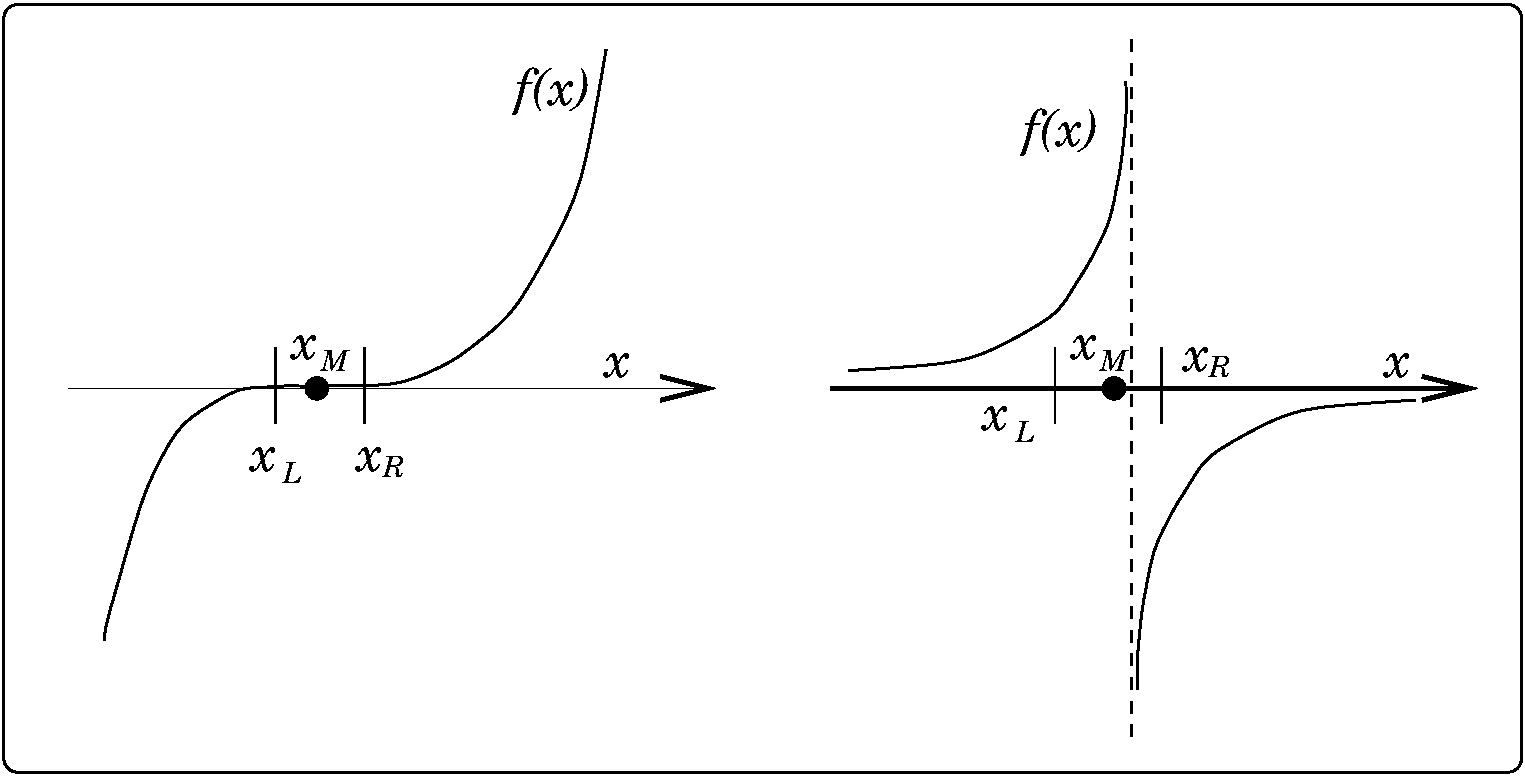
\includegraphics[width=120mm]{figures/bisec_stop}}
  \caption{\label{bisec_stop} \it In the left hand case the criterion
    $\abs{x_n^{(R)}-x_n^{(L)}} < \delta$ fails, in the right hand case the
    criterion $\abs{f(x_n^{(M)})} < \varepsilon$ fails.}
\end{figure}

\noindent
\textbf{Remark 1} - The error in the location of the root at the
$n$-th step is smaller than $(x_0^{(R)}-x_0^{(L)})/2^n$.

\noindent
\textbf{Remark 2} - This method is easy to code and it
always converges.   However, it is rather slow.

\section{Contraction mappings}

\subsection{Introduction}

Many of the methods that we will discuss for solving nonlinear
equations like
%
\begin{equation}
  f(x)=0 \label{nonlin}
\end{equation}
%
are \textit{iterative} and can be written in the form
%
\begin{equation}
  x_{n+1} = g(x_n), \label{picard}
\end{equation}
%
for some suitable function $g(x)$ and initial approximation $x_0$.
The aim of the method is to find a suitable function $g(x)$ such that
the sequence has a limit and that the limit is a root of $f(x)$:
%
\begin{equation*}
  \lim_{n \to \infty} x_n = s \quad \text{and} \quad f(s)=0.
\end{equation*}
%
Note that if the limit exists then it is also a fixed point of the map
$g(x)$:
%
\begin{equation*}
  s = \lim_{n \to \infty} x_{n+1} =
  \lim_{n \to \infty} g(x_n) =
  g \left ( \lim_{n \to \infty} x_n \right ) = g(s) .
\end{equation*}
%
For example, in the case of the nonlinear problem $f(x) = 0$ we can
define the function $g(x)$ to be
%
\begin{equation*}
  g(x) = x - f(x)
\end{equation*}
%
and use the mapping~(\ref{picard}) to attempt finding the roots of
$f(x)$.  Methods of this kind are called \textit{functional iterations
  methods} or \textit{fixed point methods}.

Graphically, the solutions of~(\ref{nonlin}) or the fixed points
of~(\ref{picard}) are the intersections between the graph of $g(x)$
and the line $y=x$ (see Figure~\ref{fig:picard}).  The iteration of
the map~(\ref{picard}) can be represented on the same graph (see
Figure~\ref{fig:picard}): in the case of the solid line path the
method is converging to the fixed point, while for the dashed line
path the method is diverging.

\begin{figure}
  \centerline{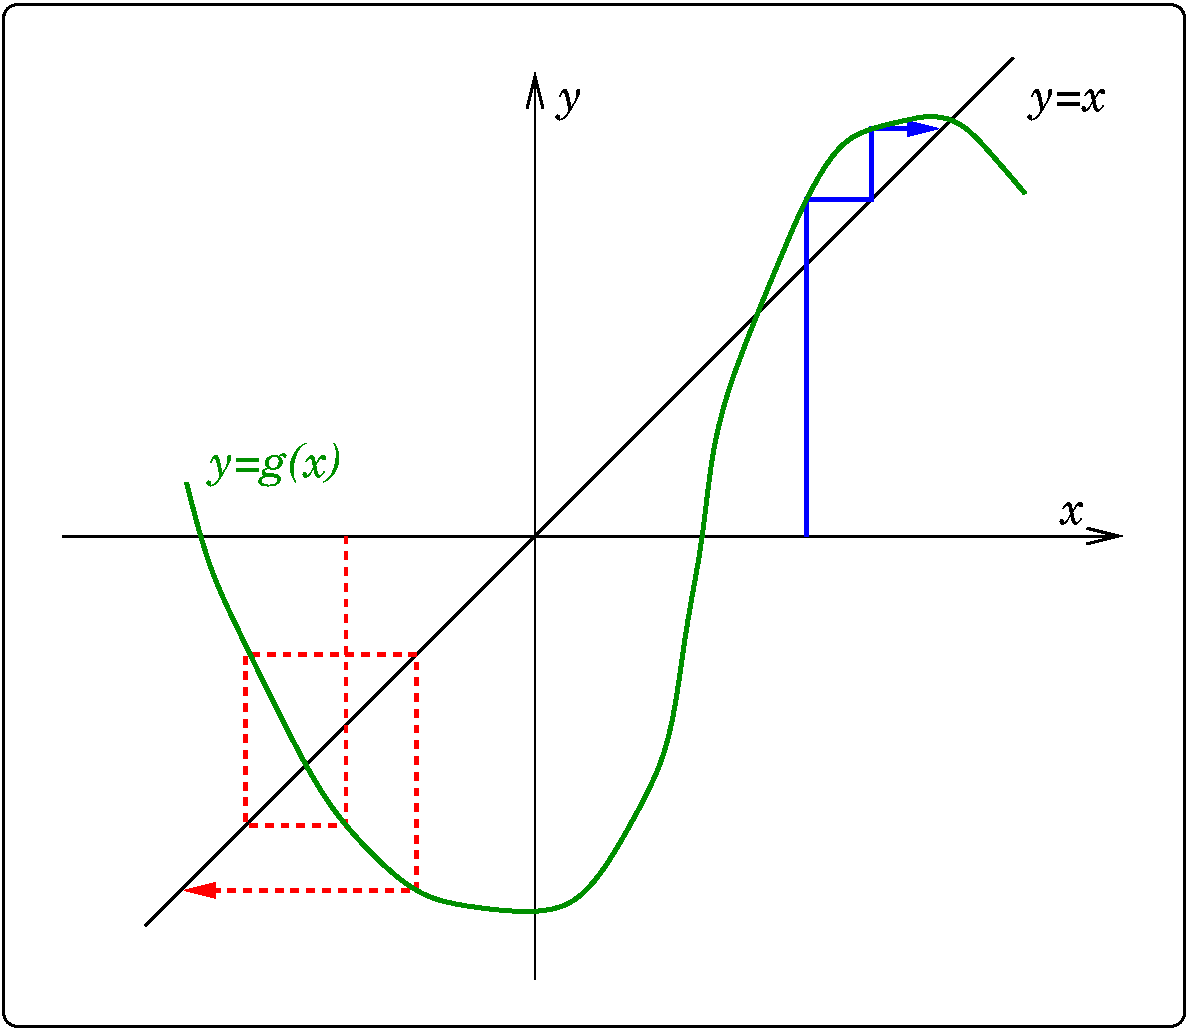
\includegraphics[width=100mm]{figures/picard}}
  \caption{\label{fig:picard} \it Graphical representation of the
    functional iteration.  The straight line paths are the graphical
    representation of the mapping~(\ref{picard}).}
\end{figure}

There are some general theorems that state under what condition the
mapping~(\ref{picard}) converges.   Before studying them, however, it
is worthwhile to make some general remarks.

\begin{itemize}
%
\item Usually iterative methods are valid for real and complex roots.
  However, in the latter case complex arithmetic must be incorporated
  into the appropriate computer codes and the initial estimate of the
  root must usually be complex.
%
\item The iterative methods require at least one initial estimate or
  guess at the location of the root being sought. If this initial
  estimate is ``sufficiently close'' to a root, then, in general, the
  procedure will converge.  The problem of how to obtain such a
  ``good'' estimate is unsolved in general.
%
\item As a general empirical rule, the schemes which converge more
  rapidly (i.e.\ higher order methods) require closer estimates.  In
  practice, these higher order schemes may require the use of more
  significant digits in order that they converge as theoretically
  predicted.  Thus, it is frequently a good idea to use a simple
  method to start with and then, when fairly close to the root, to use
  some higher order method for just a few iterations.
%
\end{itemize}

\subsection{Geometrical interpretation of fixed point schemes}

Before discussing formally what properties a map must have in order
for the iteration scheme~(\ref{picard}) to converge, we can obtain an
approximate idea by considering the four maps in
Figure~\ref{fig:contract_examples}.    From the top two maps it is
clear that in order to have a fixed point we must require $g(x)$ to be
continuous (top left) and, moreover, that the range is contained in
the domain (top right).    These requirements are not enough to have a
unique fixed point as it is shown in the bottom left corner: if the
slope of the map is too high there may be two or more fixed points.
It is only if the slope is smaller than unity that there can be only
one fixed point (bottom right corner).   Note than we do not require
that map to be differentiable: it can have as many corners as it wish.
The case of the two bottom maps is illustrated pictorially in
Figure~\ref{fig:contraction}: at each iteration the image of
the starting set $I$ gets smaller and smaller until it reduces to a
point (see Figure~\ref{fig:contraction}).

\begin{figure}
  \centerline{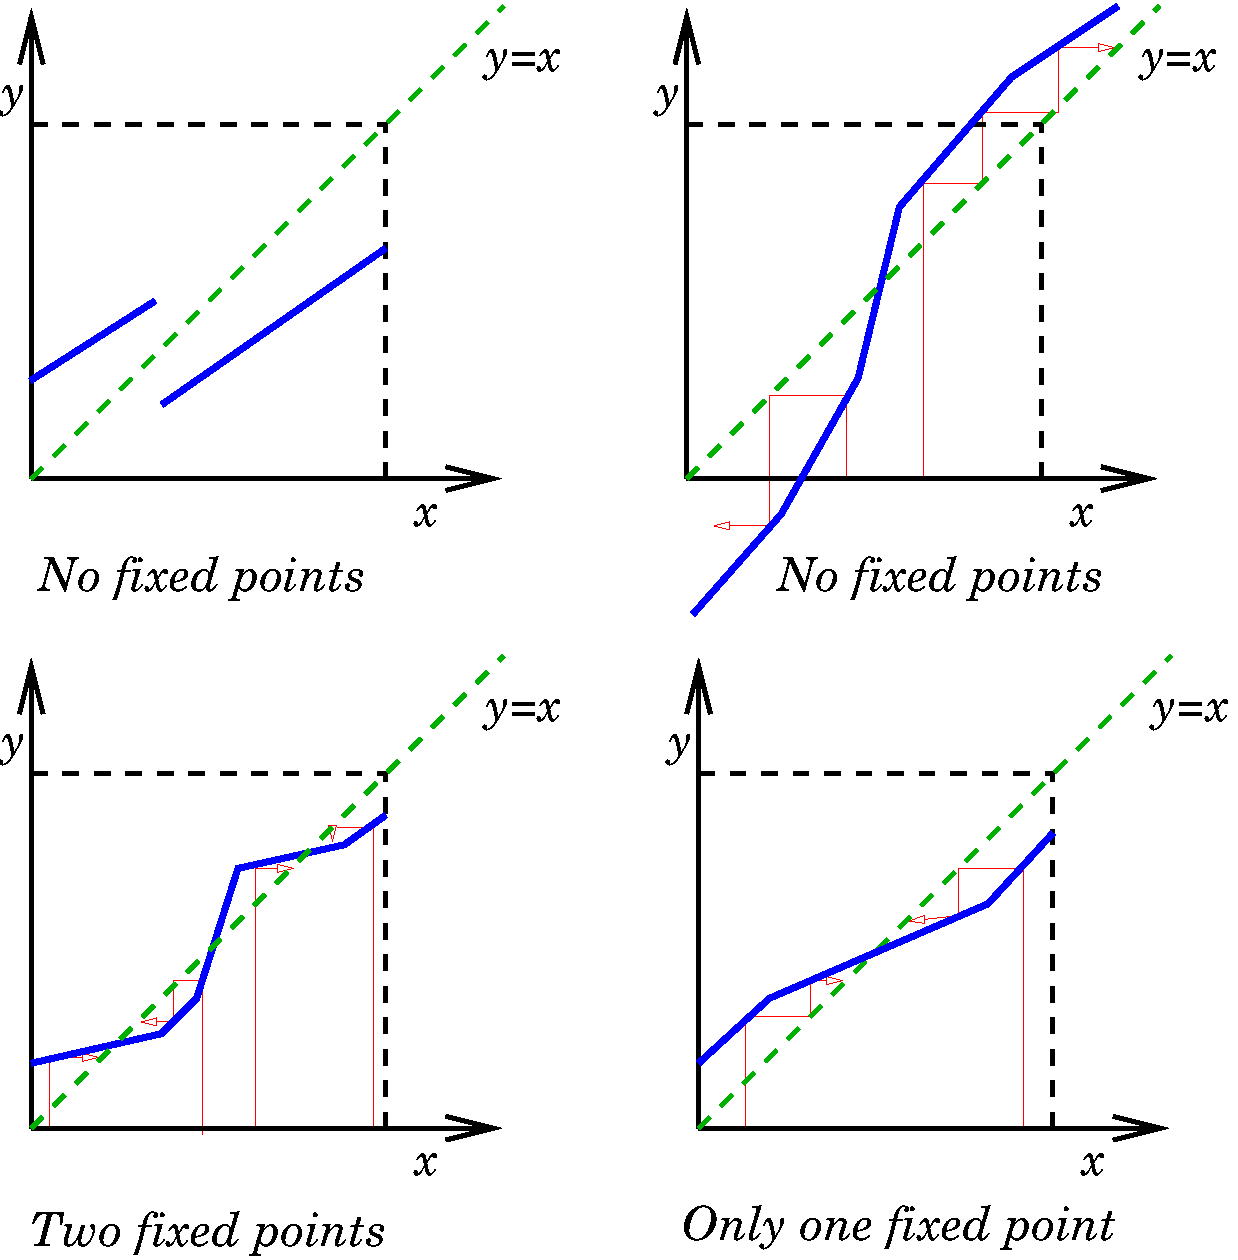
\includegraphics[width=90mm]{figures/contract_examples}}
  \caption{\label{fig:contract_examples} \it Examples of maps and
    their convergence properties.}
\end{figure}

\subsection{Definitions}

We must now phrase these intuitive results in more formal terms.   We
start by defining a contracting map.

\noindent
\textbf{Definition} - A continuous map $g(x)$ from an interval
$I=[a,b] \subseteq \bR$ into $\bR$ is \textit{contracting} if
%
\begin{enumerate}
  %
\item the image of $I$ is contained in $I$:
  %
  \begin{equation*}
    g(I) \subseteq I \quad \Leftrightarrow \quad
    g(x) \in I \, \forall x \in I .
  \end{equation*}
  %
\item the function $g(x)$ is Lipschitz continuous in $I$ with
  Lipschitz constant $L < 1$:
  %
  \begin{equation*}
    \abs{ g(x) - g(y) } \le L \abs{ x - y } \quad \forall x,y \in I .
  \end{equation*}
  %
  In other words, the distance between the images is smaller than the
  distance between the two starting points.
  %
\end{enumerate}

\noindent
\textbf{Remark 1} - A function that is Lipschitz continuous is
``more'' than continuous, but ``less'' than differentiable.  For
example, the function $f_1(x)=\sqrt{x}$ is continuous in the interval
$[0,1]$, but it is not Lipschitz.  On the other hand, the function
$f_2(x)=\abs{x}$ is Lipschitz in the interval $[-1,1]$, but it is not
differentiable at $x=0$.

\noindent
\textbf{Remark 2} - If the function $g(x)$ is differentiable and
Lipschitz continuous with constant $L$ then
%
\begin{equation*}
   \abs{\dv{g}{x}}  \le L.
\end{equation*}

\subsection{Convergence theorems}

A map that is contracting is also called a \textit{contraction
mapping}.  From the definition and Figures~\ref{fig:contract_examples}
and~\ref{fig:contraction} we can intuitively understand that if
the map $g(x)$ in~(\ref{picard}) is contracting, then we are
guaranteed convergence.  All this is expressed more
formally (and more clearly) in the following sets of theorems.

\begin{figure}
  \centerline{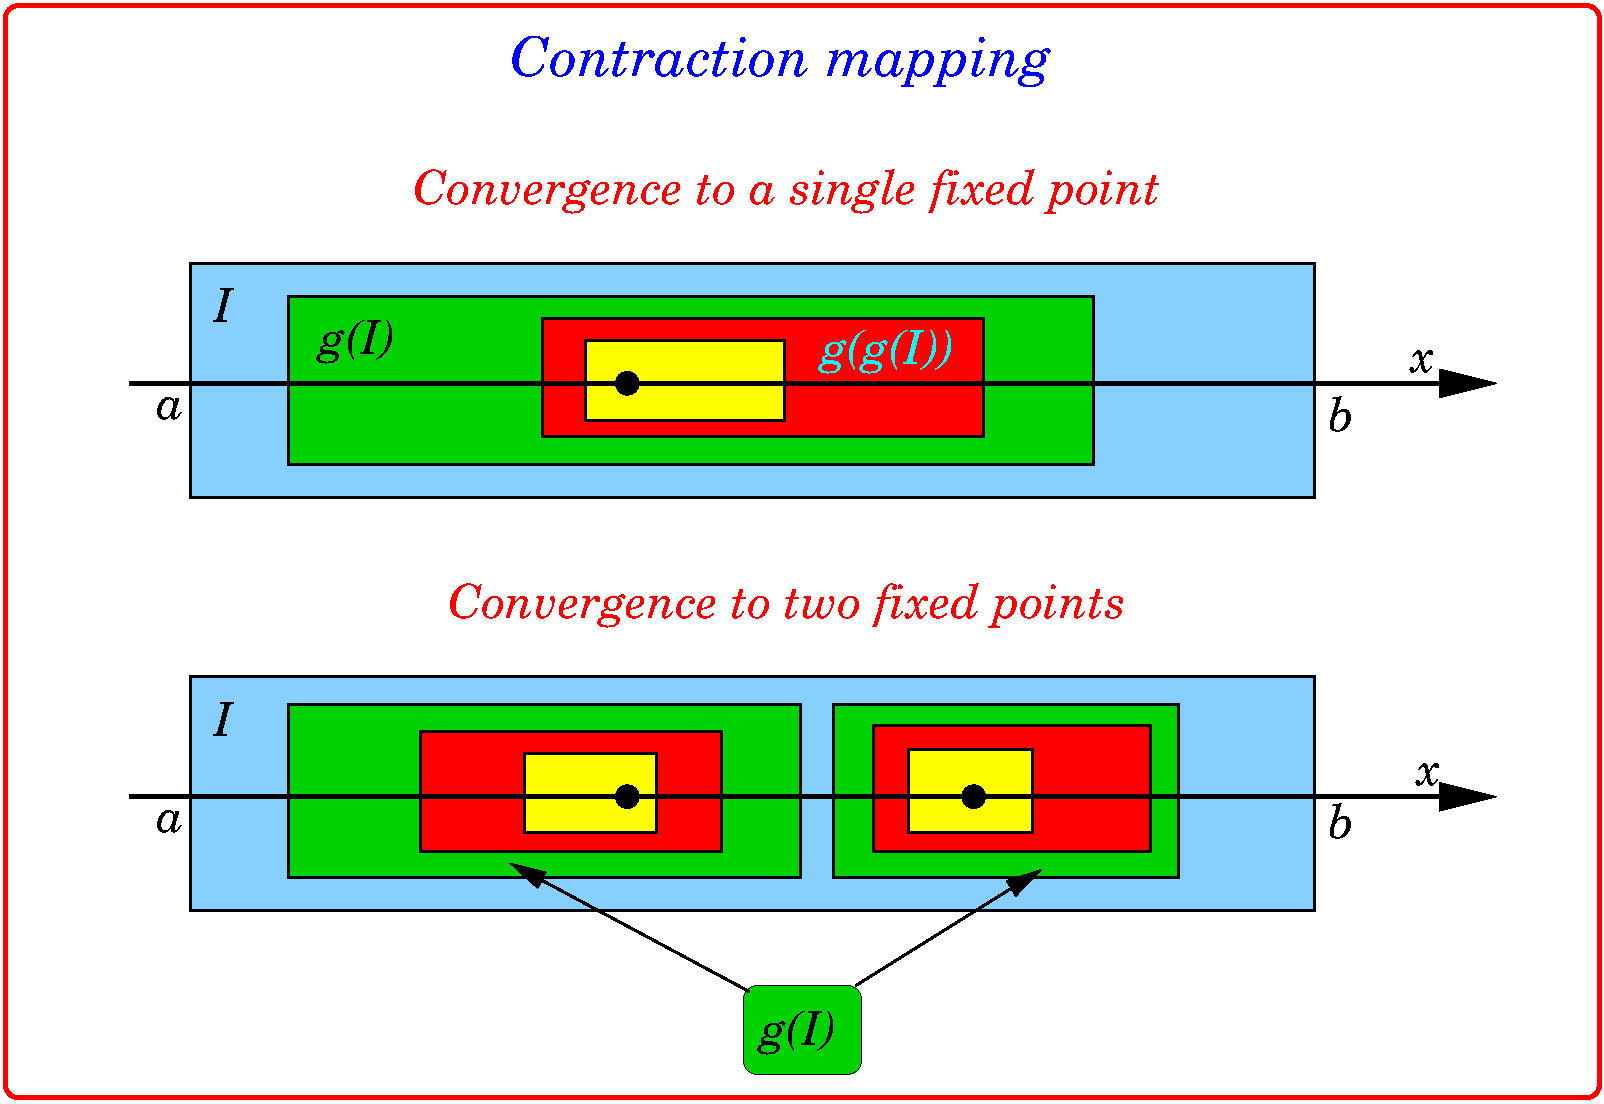
\includegraphics[width=90mm]{figures/contraction_col}}
  \caption{\label{fig:contraction} \it Graphical representation of the
    contraction mapping principle.  At each iteration the image of the
    interval gets smaller and the iterations of the contraction map
    converge towards its fixed point(s).}
\end{figure}

First of all, we prove that if the image of  the interval is contained
in the interval (without any requirement of Lipschitz continuity) then
there is at least one fixed point (but there may be many).

\smallskip

\begin{theorem}
\label{contract1}
If the function $g(x)$ is continuous in $I=[a,b]$ and $g(I) \subseteq
I$, then $g(x)$ has at least one fixed point in $I$.
\end{theorem}

\noindent
\textbf{Proof} - Since $g(I) \subseteq I$ we must have
%
\begin{equation*}
   a \le g(a) \le b \quad \text{and} \quad a \le g(b) \le b .
\end{equation*}
%
If either $g(a)=a$ or $g(b)=b$ then there is one fixed point and the
theorem is proved.   Otherwise, the following inequalities must hold:
%
\begin{equation*}
  g(a) - a \ge 0 \quad \text{and} \quad g(b) - b \le 0 .
\end{equation*}
%
Define the function $F(x) = g(x) - x$.   $F(x)$ is continuous and
$F(a) \ge 0$, while $F(b) \le 0$.   Therefore, by the intermediate
value theorem there exists a point $c \in [a,b]$ such that
%
\begin{equation*}
  F(c)=0 \implies c = g(c) .
\end{equation*}

\hfill \rule{3mm}{3mm}

\smallskip

\noindent
\textbf{Exercise} - Give a graphical representation of this theorem.
In particular show that the contraction map that would produce a graph
similar to the bottom part of Figure~\ref{fig:contraction} must have a
jump discontinuity in $[a,b]$.

\smallskip

Theorem~\ref{contract1} provides us with an important result, but not
with enough.  Ideally we would like the zero to be unique.  In order
for this to be true, we must have more stringent requirements on
$g(x)$: it must not vary too rapidly.  This is assured if $g(x)$ is
Lipschitz continuous with a sufficiently small Lipschitz constant.

\begin{theorem}[Contraction mapping theorem]
\label{contract2}
If $g(x)$ is a contraction mapping in an interval
$I=[a,b]$ then there exists one and only one fixed point of the map in
$[a,b]$.
\end{theorem}

We will prove a slightly less strong version of this theorem: we
require that the map $g(x)$ is differentiable in $I$ and that $\abs{g'(x)}
\le L < 1$.   Such a function is Lipschitz continuous of Lipschitz
constant $L$: therefore it is a contraction mapping.

\begin{theorem}
\label{contract3}
If $g(x)$ is a differentiable contraction mapping
in an interval $I=[a,b]$, i.e.
%
\begin{equation*}
  \abs{g'(x)} \le L < 1, \qquad \forall x \in [a,b] ,
\end{equation*}
%
then there exists one and only one fixed point of the map in $[a,b]$.
\end{theorem}

\noindent
\textbf{Proof} - The existence of the derivative implies that the
function $g(x)$ is continuous.  Since, by hypothesis $g(I) \subseteq
I$, then by Theorem~\ref{contract1} there is at least one fixed point,
$s_1$.  Suppose that there is another one $s_2 : s_2 = g(s_2)$ and
$s_1 \ne s_2$.  We can use the mean value
theorem\footnote{\textbf{Mean value theorem} - For any differentiable
$F(x)$ in $I \subseteq \bR$ and any $c, d \in I$ there exists a point
$\xi \in [c,d]$ such that
%
\begin{equation*}
  F'(\xi) = \frac{F(d)-F(c)}{d-c} .
\end{equation*}
}
to prove that this is impossible:
%
\begin{equation*}
  \abs{s_2 - s_1} = \abs{g(s_2) - g(s_1)} =
  \abs{g'(\xi) (s_2 - s_1)}  \le L \abs{s_2 - s_1} < \abs{|s_2 - s_1} .
\end{equation*}
%
This inequality cannot be true and therefore there can be no other
fixed point. (The proof assuming Lipschitz continuity only is
essentially identical.) \hfill \rule{3mm}{3mm}

\smallskip

The consequence of this theorem is that the algorithm represented by
the mapping~(\ref{picard}) is guaranteed to have a root in an interval
$[a,b]$ if the map is a contraction mapping in this interval.  The
following theorem tells us how to find it.

\smallskip

\begin{theorem}
\label{contract4}
Let $I=[a,b]$ and suppose that $g(x)$ is a contraction mapping in $I$.
Then for arbitrary $x_0 \in I$, the sequence $x_n = g(x_{n-1})$,
$n=1,2,\ldots$ converges to the unique fixed point, $s$, of the map.
Moreover, if the error $e_n$ at the $n$-th stage is defined by $e_n =
x_n - s$ then
%
\begin{equation*}
  \abs{e_n} \le \frac{L^n}{1-L} \abs{ x_1 - x_0 } .
\end{equation*}
\end{theorem}

\noindent
\textbf{Proof} - To prove the convergence to the fixed point, whatever
the arbitrary guess $x_0 \in I$, we use the Lipschitz property of the
map and the fact that $s=g(s$) to bound $\abs{e_n}$ from above
with a bound that tends to zero as $n$ tends to infinity.  As a first step
we have:
%
\begin{align}
  \abs{e_n} & = \abs{ x_n - s} \\
  & = \abs{ g(x_{n-1}) - g(s) } \\
  & \le L \abs{ x_{n-1} - s } \\
  & = L \abs{ e_{n-1} } .
\end{align}
%
By applying this inequality over and over again we obtain
%
\begin{align}
  \abs{ e_n } & \le L \abs{ e_{n-1} } \\
  & \le L^2 \abs{ e_{n-2} } \\
  & \le \ldots \\
  & \le L^n \abs{ e_0 } \label{ineq_conv}
\end{align}
%
By the definition of contraction mapping $L < 1$ and therefore
%
\begin{equation*}
  \lim_{n \to \infty} L^n = 0 \implies \lim_{n \to \infty} x_n = s .
\end{equation*}
%
Equation~(\ref{ineq_conv}) provides a bound on the error of the $n$-th
estimate in terms of the initial error.   Unfortunately this quantity
is not know, because we do not know the root $s$ of the equation.   We
therefore must replace $\abs{e_0}$ in~(\ref{ineq_conv}) with an expression
that we can compute, namely $\abs{x_0 - x_1}$:
%
\begin{align}
  &&  \abs{ x_0 - s } & = \abs{ x_0 - x_1 + x_1 - s } \\
  &&  & \le \abs{ x_0 - x_1 } + \abs{ x_1  - s} \\
  &&  & \le \abs{ x_0 - x_1 } + L \abs{ x_0 - s } \\
  \implies && \abs{e_0} & = \abs{ x_0 - s } \\
  && & \le \frac{\abs{ x_0 - x_1 }}{1-L}.
\end{align}
%
Using~(\ref{ineq_conv}) we obtain
%
\begin{equation}
  \abs{ e_n } \le L^n \abs{ e_0 } \le \frac{L^n}{1-L} \abs{ x_0 - x_1 } .
  \label{err_boundL}
\end{equation}
\hfill \rule{3mm}{3mm}

These four theorems are represented graphically in
Figure~\ref{fig:contract}.  Since the slope of the function $g(x)$ is
smaller than unity successive iterations of the map get closer and
closer to its fixed point.

\begin{figure}
  \centerline{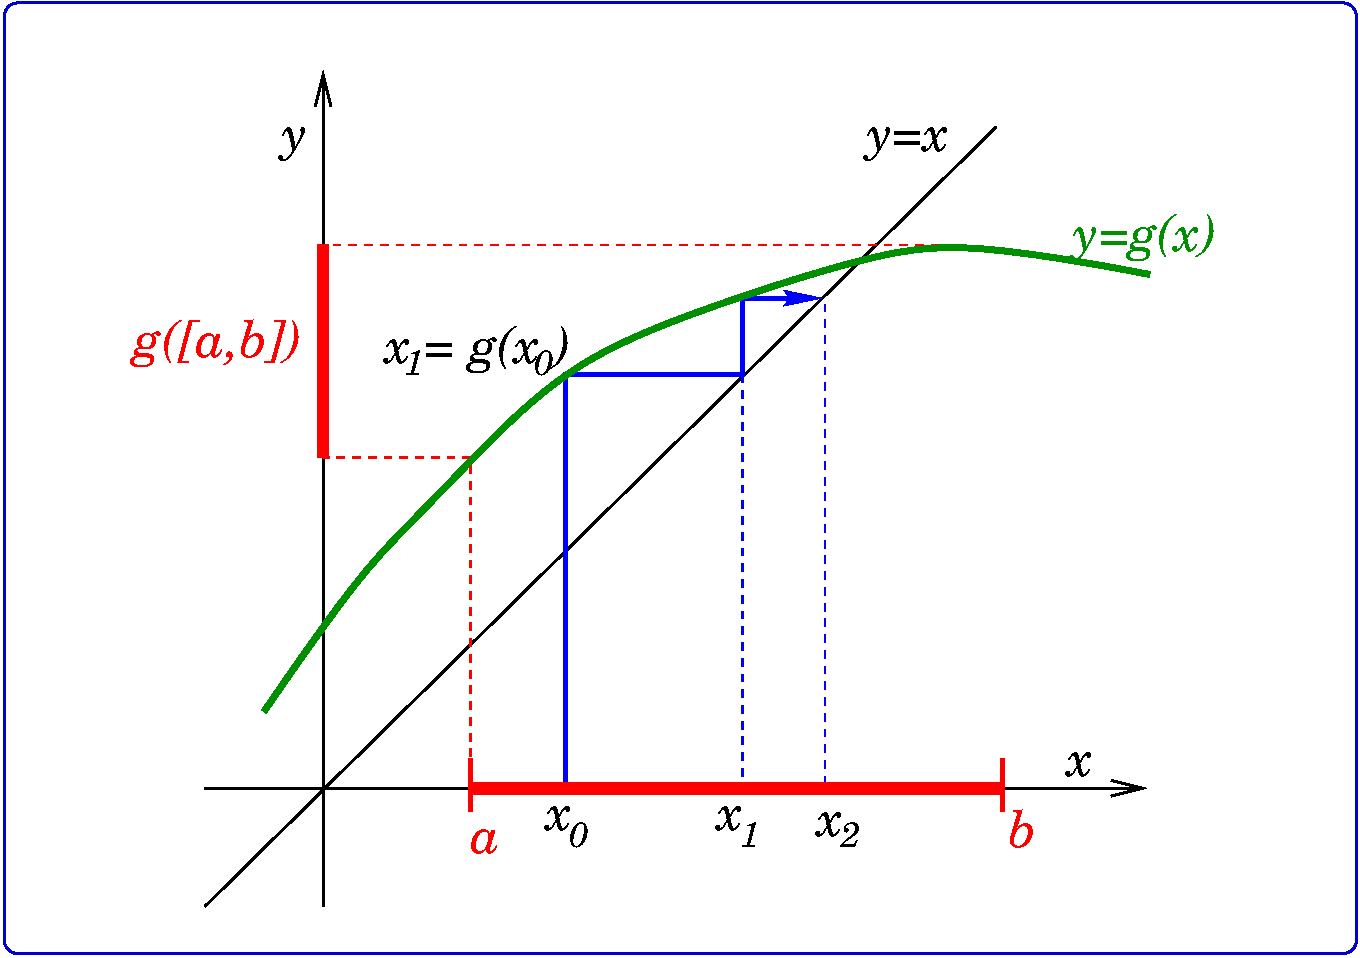
\includegraphics[width=80mm]{figures/contract}}
  \caption{\label{fig:contract} \it Graphical representation of the
    contracting mapping theorems.  The map $g(x)$ is a contraction
    mapping in $[a,b]$: the image of the interval is smaller than the
    original interval.  Each iteration of a starting guess $x_0$ gets
    closer and closer to the fixed point.}
\end{figure}

\subsection{Speed of convergence}

The bound~(\ref{err_boundL}) on the error provided by
Theorem~\ref{contract4} depends, through the Lipschitz constant $L$,
on the interval chosen to estimate the map.  Moreover, it is
reasonable to assume that the rate of convergence of the map, i.e.\ the
rate of decrease of the error $e_n$ depends only on the properties of
the map in a neighbourhood of the root.  We can show that this is
indeed the case if the map is differentiable, so that it is possible
to expand it in a Taylor polynomial: call $g(x)$ a suitably
differentiable contraction mapping in $I=[a,b]$, $s$ its fixed point,
$x_0 \in I$ the starting point of the iteration and $e_n = x_n - s$
the error at the $n$-th iteration.  Using the definition of the map
and Taylor's expansion we can write:
%
\begin{align*}
  e_{n+1} & = x_{n+1} - s \\
          & = g(x_n) - g(s) \\
          & = g'(s)(x_n-s) + \frac{g''(s)}{2!}(x_n-s)^2 + \ldots +
          \frac{g^{(k)}(s)}{k!}(x_n-s)^k + R_{n,k} \\
          & = g'(s) e_n + \frac{g''(s)}{2!} e_n^2 + \ldots +
          \frac{g^{(k)}(s)}{k!} e_n^k + R_{n,k} ,
\end{align*}
%
where $R_{n,k}$ is the remainder of the expansion:
%
\begin{equation*}
  R_{n,k} = \frac{g^{(k)}(\xi)}{k!}(x_n-s)^{k+1}, \quad
  \xi \in [x_n,s].
\end{equation*}
%
Assuming that $g'(s) \ne 0$ then
%
\begin{equation*}
  e_{n+1} \sim g'(s) e_n,
\end{equation*}
%
i.e.\ the error decreases at a constant rate at each iteration: such a
method is called \textit{linear} or \textit{first order}.  If,
instead, $g'(s)=0$, but $g''(s) \ne 0$ then
%
\begin{equation*}
  e_{n+1} \sim g''(s) e_n^2,
\end{equation*}
%
i.e.\ the error at each iteration is proportional to the square of the
previous error: such a method is called a \textit{quadratic} or
\textit{second order} method.  The more derivatives of $g(s)$ vanish
the higher the order of the method and the faster the convergence.
However, it may well be that the method will converge only if the
starting point is very close to the root.

\subsection{Error propagation}

The final question that we must answer before discussing practical
implementations of the theory we have just studied is ``Are these
theorems numerically stable?''  In other words, what is the effect of
the numerical error on the convergence properties of a contraction
map?  In actual computations it may not be possible, or practical, to
evaluate the function $g(x)$ exactly (i.e.\ only a finite number of
decimals may be retained after rounding or $g(x)$ may be given as the
numerical solution of a differential equation, etc.).  For any value
of $x$ we may then represent our approximation to $g(x)$ by $G(x) =
g(x) + \delta(x)$ where $\delta(x)$ is the error committed in
evaluating $g(x)$.  Frequently we may know a bound for $\delta(x)$,
i.e.\ $\delta(x) < \delta$.  Thus the actual iteration scheme which is
used may be represented as
%
\begin{equation}
  X_{n+1} \equiv G(X_n) = g(X_n) + \delta_n, \quad
  n = 0,1,2, \ldots, \label{Xn}
\end{equation}
%
where the $X_n$ are the numbers obtained from the calculations and the
$\delta_n \equiv \delta(X_n)$ satisfy
%
\begin{equation}
  \abs{\delta_n} \le \delta, \quad n= 0,1,2, \ldots \label{deltabound}
\end{equation}
%
We cannot expect the computed iterates $X_n$ of~(\ref{Xn}) to
converge.   However, under proper conditions, it should be possible to
approximate a root to an accuracy determined essentially by the
accuracy of the computations, $\delta$.

\begin{figure}
  \centerline{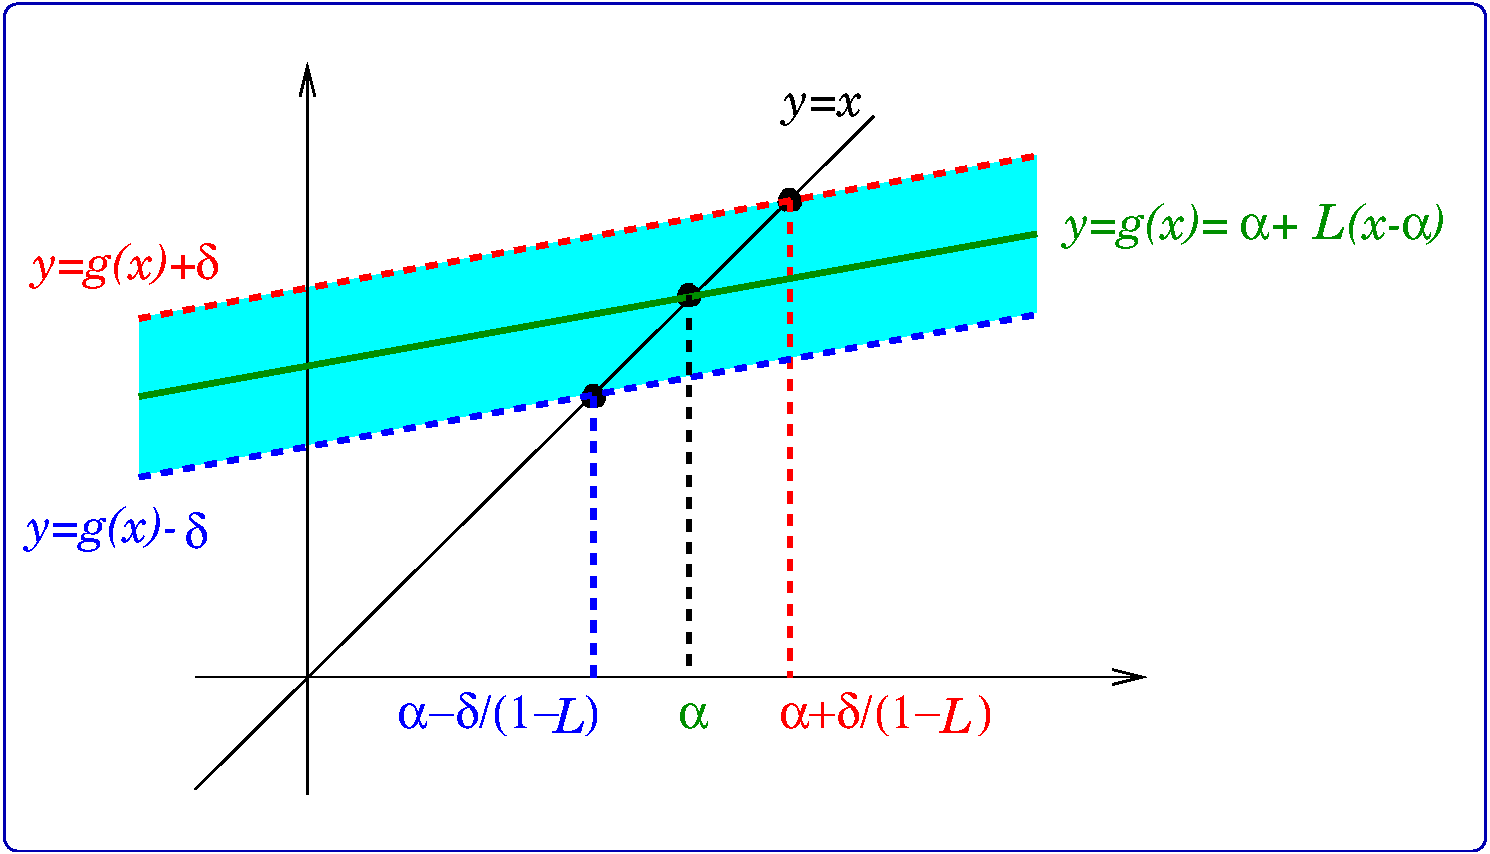
\includegraphics[width=120mm]{figures/contract_error}}
  \caption{\label{fig:contract_error} \it The width of the numerical
    error band around the fixed point of the iteration map.}
\end{figure}

For example, from Figure~\ref{fig:contract_error} we can see that for
the special case of $g(x) = \alpha + L (x-\alpha)$, the uncertainty in
the root $\alpha$ is bounded by $\pm \delta/(1 - L)$.  We note that if
the slope $L$ is close to unity the problem is not ``properly posed''.
The following theorem states quite generally that when the functional
iteration scheme is convergent, the presence of errors in computing
$g(x)$, of magnitudes bounded by $\delta$, causes the scheme to
estimate the root $\alpha$ with an uncertainty bounded by $\pm
\delta/(1-L)$, where $L$ is the Lipschitz constant of the contraction
mapping.  The phrasing of this theorem is slightly different from the
previous ones because the numerical error $\delta$ forces us to define
quite strictly the interval we want to work in: we know that $g(I)
\subseteq I$, but it is not generally true that $G(I) \subseteq I$.

\begin{theorem}
\label{contract5}
Let $g(x)$ be a contraction mapping with fixed point $s$ and let $L$
be its Lipschitz constant in the interval $I(s,r_0) \equiv
[s-r_0,s+r_0]$.  Let $\delta$ be the bound on the numerical errors of
the iterates of the numerical map~(\ref{Xn}) as defined
in~(\ref{deltabound}).  Finally, assume that the starting point of the
iteration of~(\ref{Xn}) is a point $X_0$ in the smaller interval
%
\begin{equation}
  X_0 \in I(s,R_0) \equiv [s - R_0, s + R_0] ,  \label{X0}
\end{equation}
%
where
%
\begin{equation*}
  0 < R_0 \le r_0 - \frac{\delta}{1-L} .
\end{equation*}
%
Then the iterates $X_n$ of~(\ref{Xn}) with the errors bounded
by~(\ref{deltabound}), lie in the interval $I(s,r_0)$,
and
%
\begin{equation}
  \abs{ s - X_n } \le
  \frac{\delta}{1 - L} +
  L^n \left ( R_0 - \frac{\delta}{1-L} \right ), \label{bound_err}
\end{equation}
%
where $L^n \to 0$ as $n \to \infty$.
\end{theorem}

\noindent
\textbf{Proof} - The proof of this theorem involves showing that the
numerical error does not push the iteration outside the interval
$I(s,r_0)$ where it is defined.  In the process of doing so we also
derive the bound~(\ref{bound_err}) on the error of the numerical
estimate.  The proof that the iterations are always in the interval
$I(s,r_0)$ is by induction.

The point $X_0$ is, by hypothesis, inside the interval $I(s,R_0)
\subseteq I(s,r_0)$.  We now suppose that the iterations $X_0, X_1,
\ldots, X_{n-1}$ are in $I(s,r_0)$ and proceed to show that also $X_n
\in I(s,r_0)$.  By~(\ref{Xn}) and~(\ref{deltabound}) we have
%
\begin{equation*}
  \abs{ s - X_n } \le
    \abs{ [g(s) - g(X_{n-1}) ] - \delta_{n-1}  } \le
  \abs{ [g(s) - g(X_{n-1}) ]  } + \delta .
\end{equation*}
%
Since $g(x)$ is a contraction mapping of Lipschitz constant $L$  we
can write
%
\begin{align*}
  \abs{ s - X_n } & \le L \abs{ s - X_{n-1} } + \delta \\
  & \le L^2 \abs{ s - X_{n-2} } + L \delta + \delta \\
  & \le L^n \abs{ s - X_0} + ( L^{n-1} + \ldots 1 ) \delta \\
  & =  L^n \abs{ s - X_0} + \frac{1-L^n}{1-L} \delta .
\end{align*}
%
Hypothesis~(\ref{X0}) implies that $\abs{s - X_0} \le R_0$ so that
%
\begin{align}
  \abs{ s - X_n } & \le L^n R_0 + \frac{1-L^n}{1-L} \delta  \label{be1} \\
  & = L^n R_0 + \frac{\delta}{1-L} - L^n \frac{\delta}{1-L} \nonumber \\
  & \le R_0  + \frac{\delta}{1-L} \nonumber \\
  & \le r_0. \nonumber
\end{align}
Thus all the iterates are in the interval $I(s,r_0)$ and the iteration
process is defined.   Moreover~(\ref{be1}) can be rewritten
as~(\ref{bound_err}), thus completing the proof. \hfill \rule{3mm}{3mm}

\smallskip

\noindent
\textbf{Remark} - Theorem~\ref{contract5} shows that the method is
``as convergent as possible'', that is, the computational errors which
arise from the evaluation of $g(x)$ may cumulatively produce an error
of magnitude at most $\delta/(1-L)$.  Moreover, such errors limit the
size of the error bound \textit{independently of the number of
iterations}.  Therefore, it is pointless to iterate the map until $L^n
r_0 \ll \delta/(1-L)$.

\section{Examples of iteration procedures}

\subsection{Introduction}

We  have completed the  theoretical  introduction to the
numerical solution of nonlinear  equations.  We must now discuss  some
of the  algorithms  that apply  the   theory that  we have  developed.

\subsection{The chord method (first order)}

The chord method and Newton's methods are examples of the application
of the contraction mapping theorems.  Both these methods can be
introduced using a general and elegant framework.  As usual we suppose
that we have to solve the nonlinear equation
%
\begin{equation*}
  f(x) = 0,
\end{equation*}
%
in some interval $a \le x \le b$.  To define the different methods to
solve this problem we introduce a function $\varphi(x)$ such that
%
\begin{equation}
  0 < \varphi(x) < \infty, \quad x \in [a,b] ,
 \label{phibound}
\end{equation}
%
and we use it to construct a contraction mapping $x_{n+1} =
g(x_n)$, where
%
\begin{equation}
  g(x) = x - \varphi(x) f(x).   \label{gphi}
\end{equation}
%
The fixed points of the map $g(x)$ are the roots of the function
$f(x)$.

\smallskip

The simplest choice for $\varphi(x)$ in~(\ref{gphi}) is to take
%
\begin{align}
  && \varphi(x) & \equiv m \ne 0, \\
  \implies && g(x) & = x - m f(x) \\
  \implies && x_{n+1} & = x_n - m f(x_n)
  \label{phichord}
\end{align}
%
where $m$ is a number that we must choose appropriately in order for
$g(x)$ to be a contraction mapping in $[a,b]$.   The range of $m$
depends on the slope of $f(x)$ in the interval $[a,b]$.   From
Theorem~\ref{contract3} we know that $g(x)$ is a contraction mapping if
%
\begin{align}
  & &  \abs{ g'(x) } & < 1 &  \forall x &\in [a,b] \nonumber
  \\
  \implies &&
  \abs{ 1 - m f'(x) } & < 1 & \forall x &\in [a,b] \nonumber
  \\
  \implies && 0 < m f'(x) & < 2 & \forall x &\in [a,b] . \label{ineq_chord}
\end{align}
%
Thus $m$ must have the same sign as $f'(x)$, while if $f'(x)=0$ the
inequality cannot be satisfied.

The iterates of~(\ref{phichord}) have a geometrical realisation in
which the value $x_{n+1}$ is the $x$ intercept of the line with slope
$1/m$ through $(x_n,f(x_n))$ (see Figure~\ref{fig:chord}).   The
inequality~(\ref{ineq_chord}) implies that this slope should be
between $\infty$ (i.e.\ vertical) and $f'(x)/2$ (i.e.\ half the slope of
the tangent to the curve $y=f(x)$).   It is from this geometric
description that the name chord method is derived - the next iterate
is determined by a chord of constant slope joining a point on the
curve to the $x$-axis.

\begin{figure}
  \centerline{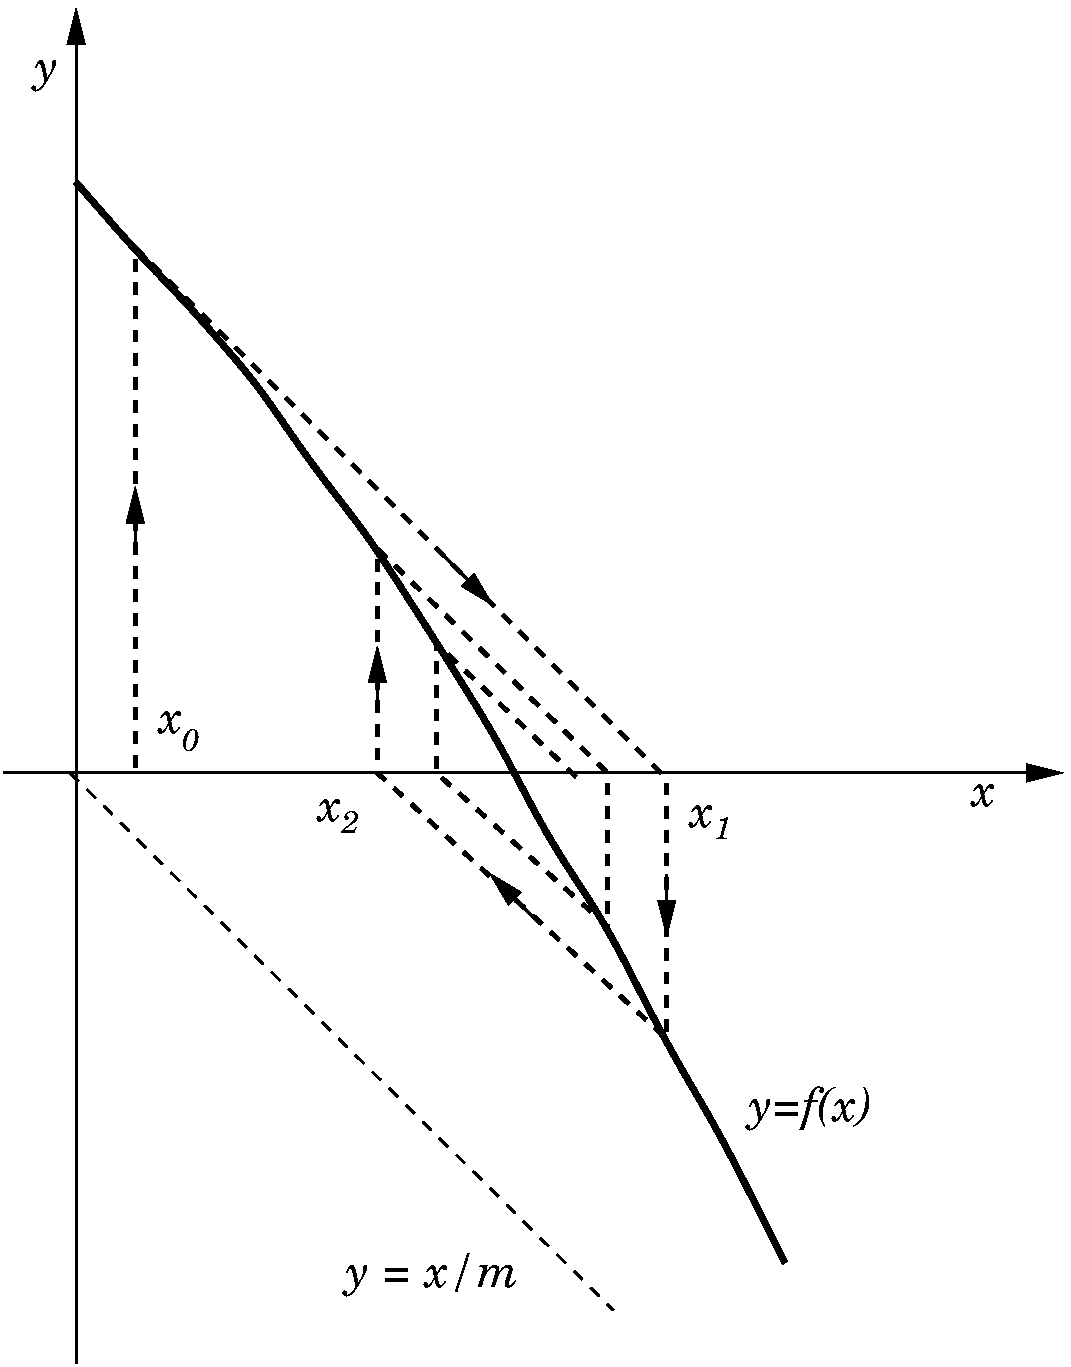
\includegraphics[width=60mm]{figures/chord}}
  \caption{\label{fig:chord} \it Geometrical representation of the
    chord method: each new iterate is determined by a chord of
    constant slope joining a point on the curve to the $x$-axis.}
\end{figure}

\medskip

\subsection{Newton's method (second order)}

The idea behind Newton's method is to chose the function $\varphi(x)$
in order that the derivative of the iteration mapping $g(x)$ is zero
at the root $x=s$.  This is ensured by the choice
%
\begin{equation}
  \varphi(x) = \frac{1}{f'(x)} \implies
  g(x) = x - \frac{f(x)}{f'(x)} , \label{gnewt}
\end{equation}
%
so that the iteration procedure is
%
\begin{equation}
  x_{n+1} = x_n - \frac{f(x_n)}{f'(x_n)} .
  \label{Newton}
\end{equation}
%
This root finding algorithm is called Newton's method.
Theorem~\ref{contract3} guarantees that the method converges in an
interval $[a,b]$ containing the root provided that $\abs{g'(x)} < 1$ in
the interval.  It is at least second order at the root $s$ of the
equation $f(x) = 0$, if $f'(s) \ne 0$ and $f''(x)$ exists, since
%
\begin{equation}
  g'(s) = \frac{f(s) f''(s)}{[f'(s)]^2} = 0 .
  \label{gpalpha}
\end{equation}
%
The geometrical interpretation of this scheme simply replaces the
chord in Figure~\ref{fig:chord} by the tangent to the line to $y=f(x)$
at $x_n,f(x_{n+1})$ (see Figure~\ref{fig:Newton}).

\begin{figure}
  \centerline{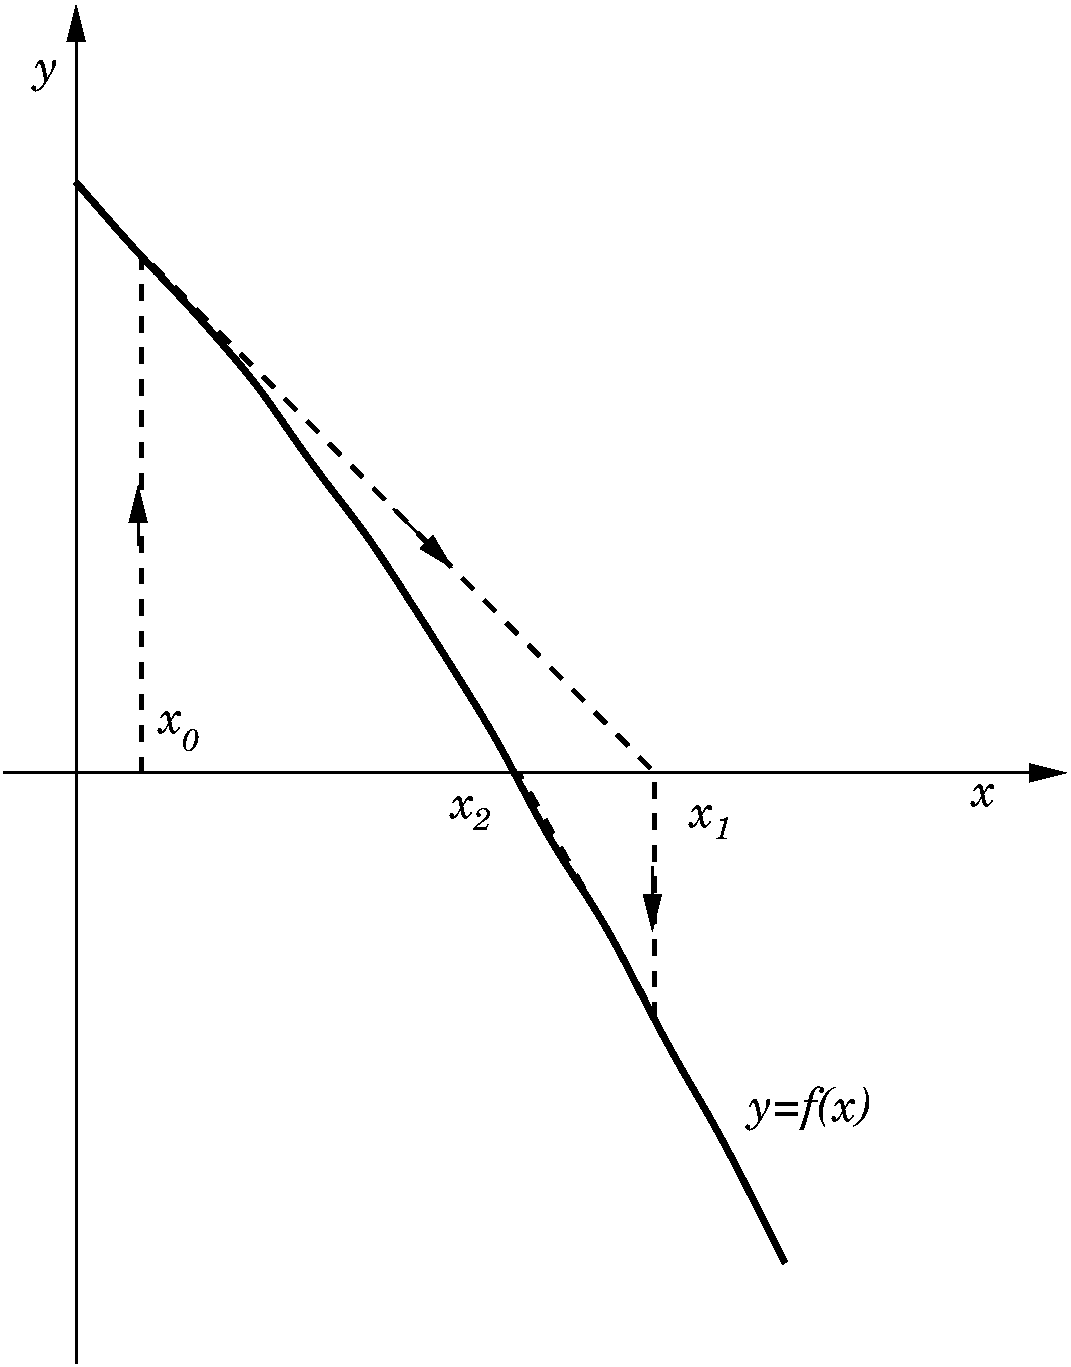
\includegraphics[width=80mm]{figures/Newton}}
  \caption{\label{fig:Newton} \it Geometrical representation of
    Newton's method: each new iterate is intersection of the tangent
    to the graph of $f(x)$ with the $x$-axis.}
\end{figure}

\noindent
\textbf{Remark 1} - It should be noted that Newton's method may be
undefined and the condition~(\ref{phibound}) violated if $f'(x)=0$ for
some $x \in [a,b]$.  In particular, if at the root $x=s$, $f'(s) = 0$,
the procedure may no longer be of second order since the hypotheses
that lead to~(\ref{gpalpha}) are not satisfied.  To examine this case
we assume that $f(x)$ has a root of multiplicity $p$ at $x=s$.  In
other words we can write,
%
\begin{equation*}
  f(x) = (x-s)^p h(x), \quad p > 1 ,
\end{equation*}
%
where the function $h(x)$ has a second derivative and $h(s) \ne 0$.
If we substitute this expression in the definition of $g(x)$
in~(\ref{gnewt}) we find that
%
\begin{equation*}
  \abs{g'(s)} = 1 - \frac{1}{p} .
\end{equation*}
%
So only in the case of a linear root, i.e.\ $p=1$ is Newton's method
second order, but it will converge as a first order method in the
general case $p \ne 1$.

\noindent
\textbf{Remark 2} - Convergence is quadratic only if we are close to
the root $s$.

\noindent
\textbf{Remark 3} - The advantage of Newton's method with respect to
the bisection (and chord) method is the faster convergence.  The main
disadvantage with respect to the bisection method is that we need to
start relatively close to the root in order to be sure that the method
will converge.

\subsection{Secant method (fractional order)}

Newton's method requires the evaluation of the derivative of the
function $f(x)$ whose root we want to find.  To do this may be very
complicated and time consuming: the secant method obviates this
problem by approximating the derivative of $f'(x)$ with the quotient
%
\begin{equation}
  f'(x_n) \simeq
  \frac{f \left (x_n \right ) - f \left ( x_{n-1} \right )}
  {x_n - x_{n-1}} .
  \label{approx_der}
\end{equation}
%
This approximation comes directly from the definition of the derivative
of $f(x)$ as the limit
%
\begin{equation*}
  f'(x) = \lim_{u \to x} \frac{f(u)-f(x)}{u-x} .
\end{equation*}
%
Substituting~(\ref{approx_der}) into the algorithm~(\ref{Newton}) for
Newton's method we obtain the secant method, namely:
%
\begin{equation}
  x_{n+1} = x_n -
  f(x_n) \frac{x_n - x_{n-1}}{f(x_n) - f (x_{n-1})} .
  \label{secant}
\end{equation}
%
The graphical interpretation of the secant method is similar to that
of Newton's method.  The tangent line to the curve is replaced by the
secant line (see Figure~\ref{fig:secant}).

\begin{figure}
  \centerline{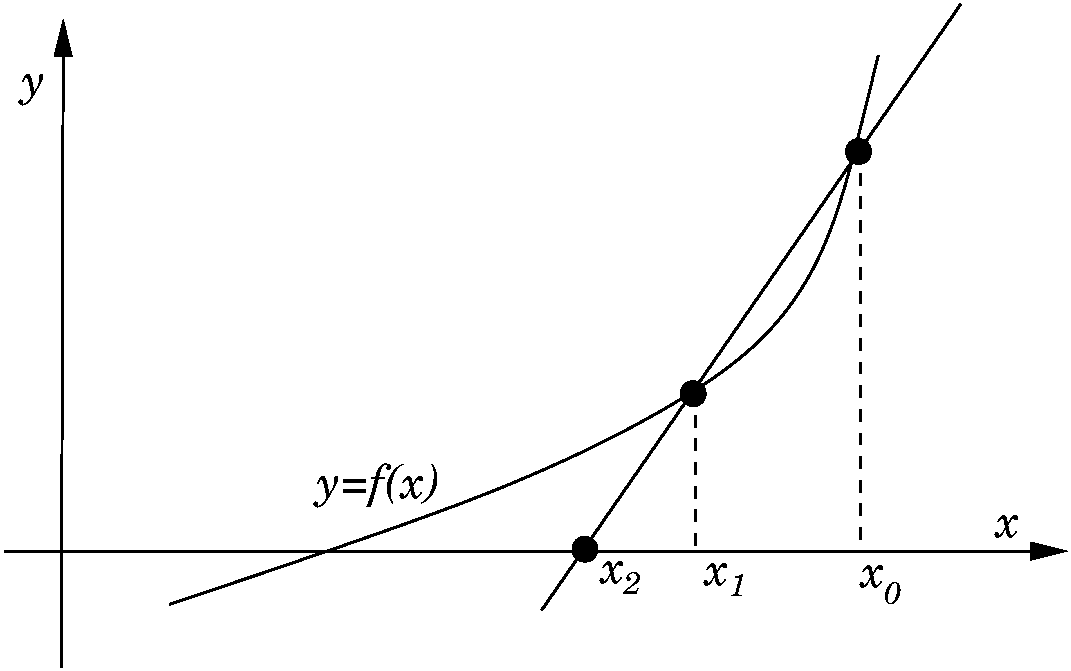
\includegraphics[width=90mm]{figures/secant}}
  \caption{\label{fig:secant} \it Geometrical representation of the
    secant method: each new iterate is intersection of the secant to
    the graph of $f(x)$ with the $x$-axis.}
\end{figure}

\noindent
\textbf{Remark 1} - This method requires two initial guesses:
$x_0$ and $x_1$.

\noindent
\textbf{Remark 2} - The convergence of the secant method cannot be
analysed using the contraction mapping theorems that we have studied
because the method cannot be put in the form $x_{n+1} = g(x_n)$: each
new iterate is a function of the previous \textbf{two}: $x_{n+1} =
g(x_n, x_{n-1})$.

\noindent
\textbf{Remark 3} - It is possible to show that the
error in the approximation decreases asymptotically as
%
\begin{equation*}
  \abs{e_{n+1}} \sim \abs{e_n}^{(1+\sqrt{5})/2} .
\end{equation*}
%
Since $(1+\sqrt{5})/2 \simeq 1.62$ the secant method is a super-linear
(i.e.\ faster than linear), but slower than quadratic convergence.
This would suggests that the secant method is slower than Newton's
method in reaching a given accuracy.  However, Newton's method
requires two function evaluations per iteration step, while the secant
method requires only one.  Therefore, when comparing the execution
speed of the two methods we should/could compare \textit{two} steps of
the secant methods with one step of Newton's method.  The rate of
decrease of the error in two steps of the secant method is $1.62^2
\simeq 2.6$ which is better than the convergence rate of Newton's
method.

\section{Systems of nonlinear equations}

\subsection{Introduction}

Finding the solutions of a systems of nonlinear equations,
%
\begin{equation*}
  \begin{cases}
    f_1(x_1, x_2, \ldots, x_n) = 0 , \\
    f_2(x_1, x_2, \ldots, x_n) = 0 , \\
    \vdots \\
    f_n(x_1, x_2, \ldots, x_n) = 0 ,
  \end{cases}
 \quad \Leftrightarrow \quad
 \bff(\bx) = 0 ,
\end{equation*}
%
is considerably more difficult that solving a single nonlinear
equation or solving a system of linear equations:

\begin{enumerate}
  %
\item The system may have \textit{no solution}, like for example
  %
  \begin{align*}
    \left\{
      \begin{aligned}
        x_1^2 + 2 x_1 x_2 + x_2^2 & = 3, \\
        x_1^3 + 3 x_1^2 x_2 + 3 x_1 x_2^2 + x_2^3 & = 4,
      \end{aligned}
    \right. &  \Longleftrightarrow \left\{
      \begin{aligned}
        (x_1 + x_2)^2 & = 3, \\
        (x_1 + x_2)^3 & = 4,
      \end{aligned}
    \right. \\
  \intertext{or have \textit{no real solutions}, like for example,}
    \left\{
      \begin{aligned}
        x_1^2 + x_2^2 & = -5, \\
        x_1^2 - 3 \, x_2^2 & = 11,
      \end{aligned}
    \right. &  \Longleftrightarrow \left\{
      \begin{aligned}
        x_1 & = \pm \tj , \\
        x_2 & = \pm 2 \tj ,
      \end{aligned}
    \right. \\
  \intertext{or have a \textit{unique solution}}
    \left\{
      \begin{aligned}
        x_1^2 + x_2^2 & = 0, \\
        \cos(x_1 x_2) & = 1,
      \end{aligned}
    \right. &  \Longleftrightarrow \left\{
      \begin{aligned}
        x_1 = 0 , \\
        x_2 = 0 ,
      \end{aligned}
    \right. \\
  \intertext{or have \textit{many solutions}}
    \left\{
      \begin{aligned}
        x_1^2 + x_2^2 & = 1, \\
        \cos[\pi(x_1^2 + x_2^2)] + x_1^2 + x_2^2 & = 0,
      \end{aligned}
    \right. &  \Longleftrightarrow
    \parbox{50mm}{all $x_1$ and $x_2$ that belong to the circle $x_1^2 +
      x_2^2 = 1$.}
  \end{align*}
  %
\item If the system is large, even the existence of a solution is
  quite unclear.
  %
\item For many real world problems the methods used to find the
  solutions can be rather ad hoc.
  %
\end{enumerate}

\subsection{Contraction mapping}

One can extend to more than one dimension the theorems on contraction
mapping that have been discussed so far.  The contraction map is now a
set of $n$ nonlinear functions in $n$ variables,
%
\begin{equation*}
  \bx_{n+1} = \bg(\bx_n) .
\end{equation*}
%
Essentially everything carries over by replacing scalars with vectors
and absolute values with norms.

We define an \textit{interval} in $\bRn$ as a set $I = \{ \bx \in \bRn
| \, a_j < x_j < b_j, \, j=1,2,\ldots, n \}$ where $a_j$ and $b_j$ are
given constants.  A \textit{contraction map} in $\bRn$ is defined as:

\noindent
\textbf{Definition} - A continuous map $\bg(\bx)$ from an interval
$I \subseteq \bRn$ into $\bRn$ is \textit{contracting} if
%
\begin{enumerate}
  %
\item the image of $I$ is contained in $I$:
  %
  \begin{equation*}
    \bg(I) \subseteq I \quad \Leftrightarrow \quad
    \bg(x) \in I \quad \forall \bx \in I .
  \end{equation*}
  %
\item the function $\bg(\bx)$ is Lipschitz continuous in $I$ with
  Lipschitz constant $L < 1$:
  %
  \begin{equation*}
    \norm{ \bg(\bx) - \bg(\by) } \le L \norm{ \bx - \by } \quad
    \forall \bx,\by \in I .
  \end{equation*}
%
\end{enumerate}

The convergence theorems are modified as follows:

\smallskip

\begin{theorem}
\label{contract1Rn}
If the function $\bg(\bx)$ is continuous in $I \subseteq \bRn$ and
$\bg(I) \subseteq I$, then $\bg(\bx)$ has at least one fixed point in
$I$.
\end{theorem}

\begin{theorem}[Contraction mapping theorem in $\bRn$]
\label{contract2Rn}
If $\bg(\bx)$ is a contraction mapping in an interval $I \subseteq
\bRn$ then there exists one and only one fixed point of the map in
$I$.
\end{theorem}

\begin{theorem}
\label{contract3Rn}
If $\bg(\bx)$ is a differentiable contraction mapping
in an interval $I \subseteq \bRn$, i.e.
%
\begin{equation*}
  \abs{\pdv{g_i}{x_j}} \le \frac{L}{n}, \quad
  \forall \bx \in I, \quad \forall i,j \quad L < 1 ,
\end{equation*}
%
then there exists one and only one fixed point of the map in $I$.
\end{theorem}

\noindent
\textbf{Remark} - The condition on the derivative can be relaxed
somewhat.   For example the theorem holds if $\norm{J(\bx)}_\infty \le
L$, where $J(\bx)$ is the Jacobian matrix of the map $\bg(\bx)$.

\smallskip

\begin{theorem}
\label{contract4Rn}
Let $I \subseteq \bRn$ be an interval in $\bRn$ and suppose that
$\bg(\bx)$ is a contraction mapping in $I$ with Lipschitz constant $L
< 1$..  Then for arbitrary $\bx_0 \in I$, the sequence $\bx_n =
\bg(\bx_{n-1})$, $n=1,2,\ldots$ converges to the unique fixed point,
$\bs$, of the map.  Moreover, if the error $\be_n$ at the $n$-th stage
is defined by $\be_n = \bx_n - \bs$ then
%
\begin{equation*}
  \norm{ \be_n }_\infty \le \frac{L^n}{1-L} \norm{ \bx_1 - \bx_0 }_\infty .
\end{equation*}
%
\end{theorem}

\smallskip

\noindent
\textbf{Exercise} - Show that
%
\begin{equation}
  \label{eq:contRnex}
  \bg(\bx) = \left\{
    \begin{aligned}
      g_1(x_1,x_2,x_3) & = \dfrac{1}{3} \cos(x_2 x_3) + \dfrac{1}{6} , \\
      g_2(x_1,x_2,x_3) & =
      \dfrac{1}{9} \sqrt{x_1^2 + \sin(x_3) + 1.06} - 0.1, \\
      g_3(x_1,x_2,x_3) & =
      -\dfrac{1}{20} e^{-x_1 x_2} - \left ( \dfrac{10 \pi -3}{60} \right ),
    \end{aligned}
    \right.
\end{equation}
%
satisfies all the conditions of theorem~\ref{contract3Rn} in $-1 < x_i <
1$.

\smallskip

\noindent
\textbf{Remark 1} - In practice it may be rather tough to prove that
$g(I) \subseteq I$.

\noindent
\textbf{Remark 2} - There is a ``Gauss-Seidel'' version of this
method, where each iterate is used as soon as it becomes available.

\noindent
\textbf{Remark 3} - The analogy with linear systems extends to the
S.O.R. method.  It is often hard to get the direct iteration to
converge.  However, the convergence can be helped by using
``relaxation'' (the opposite of S.O.R.).  This method introduces an
``under-relaxation'' parameter $\omega < 1$ in the iteration.
Assuming that we know the iterate $\bx_n$ we compute a first estimate
of the iterate $n+1$, $\hat \bx_{n+1}$ using the iteration map
$\bg(\bx)$:
%
\begin{equation*}
  \hat \bx_{n+1} = \bg(\bx_n) .
\end{equation*}
%
Use this estimate to obtain $\bx_{n+1}$ according to
%
\begin{equation*}
  \bx_{n+1} = \bx_n + \omega ( \hat \bx_{n+1} - \bx_n ) .
\end{equation*}
%
This procedure effectively multiplies the derivatives of the map
$\bg(\bx)$ by $\omega < 1$.  If $\omega = 1$ this procedure reduces to
the standard contraction mapping.

The drawback of this method is that sometimes $\omega$ has to be made
so small that convergence is slow and too many iterations are needed.


\subsection{Newton's method}

\begin{figure}
  \centerline{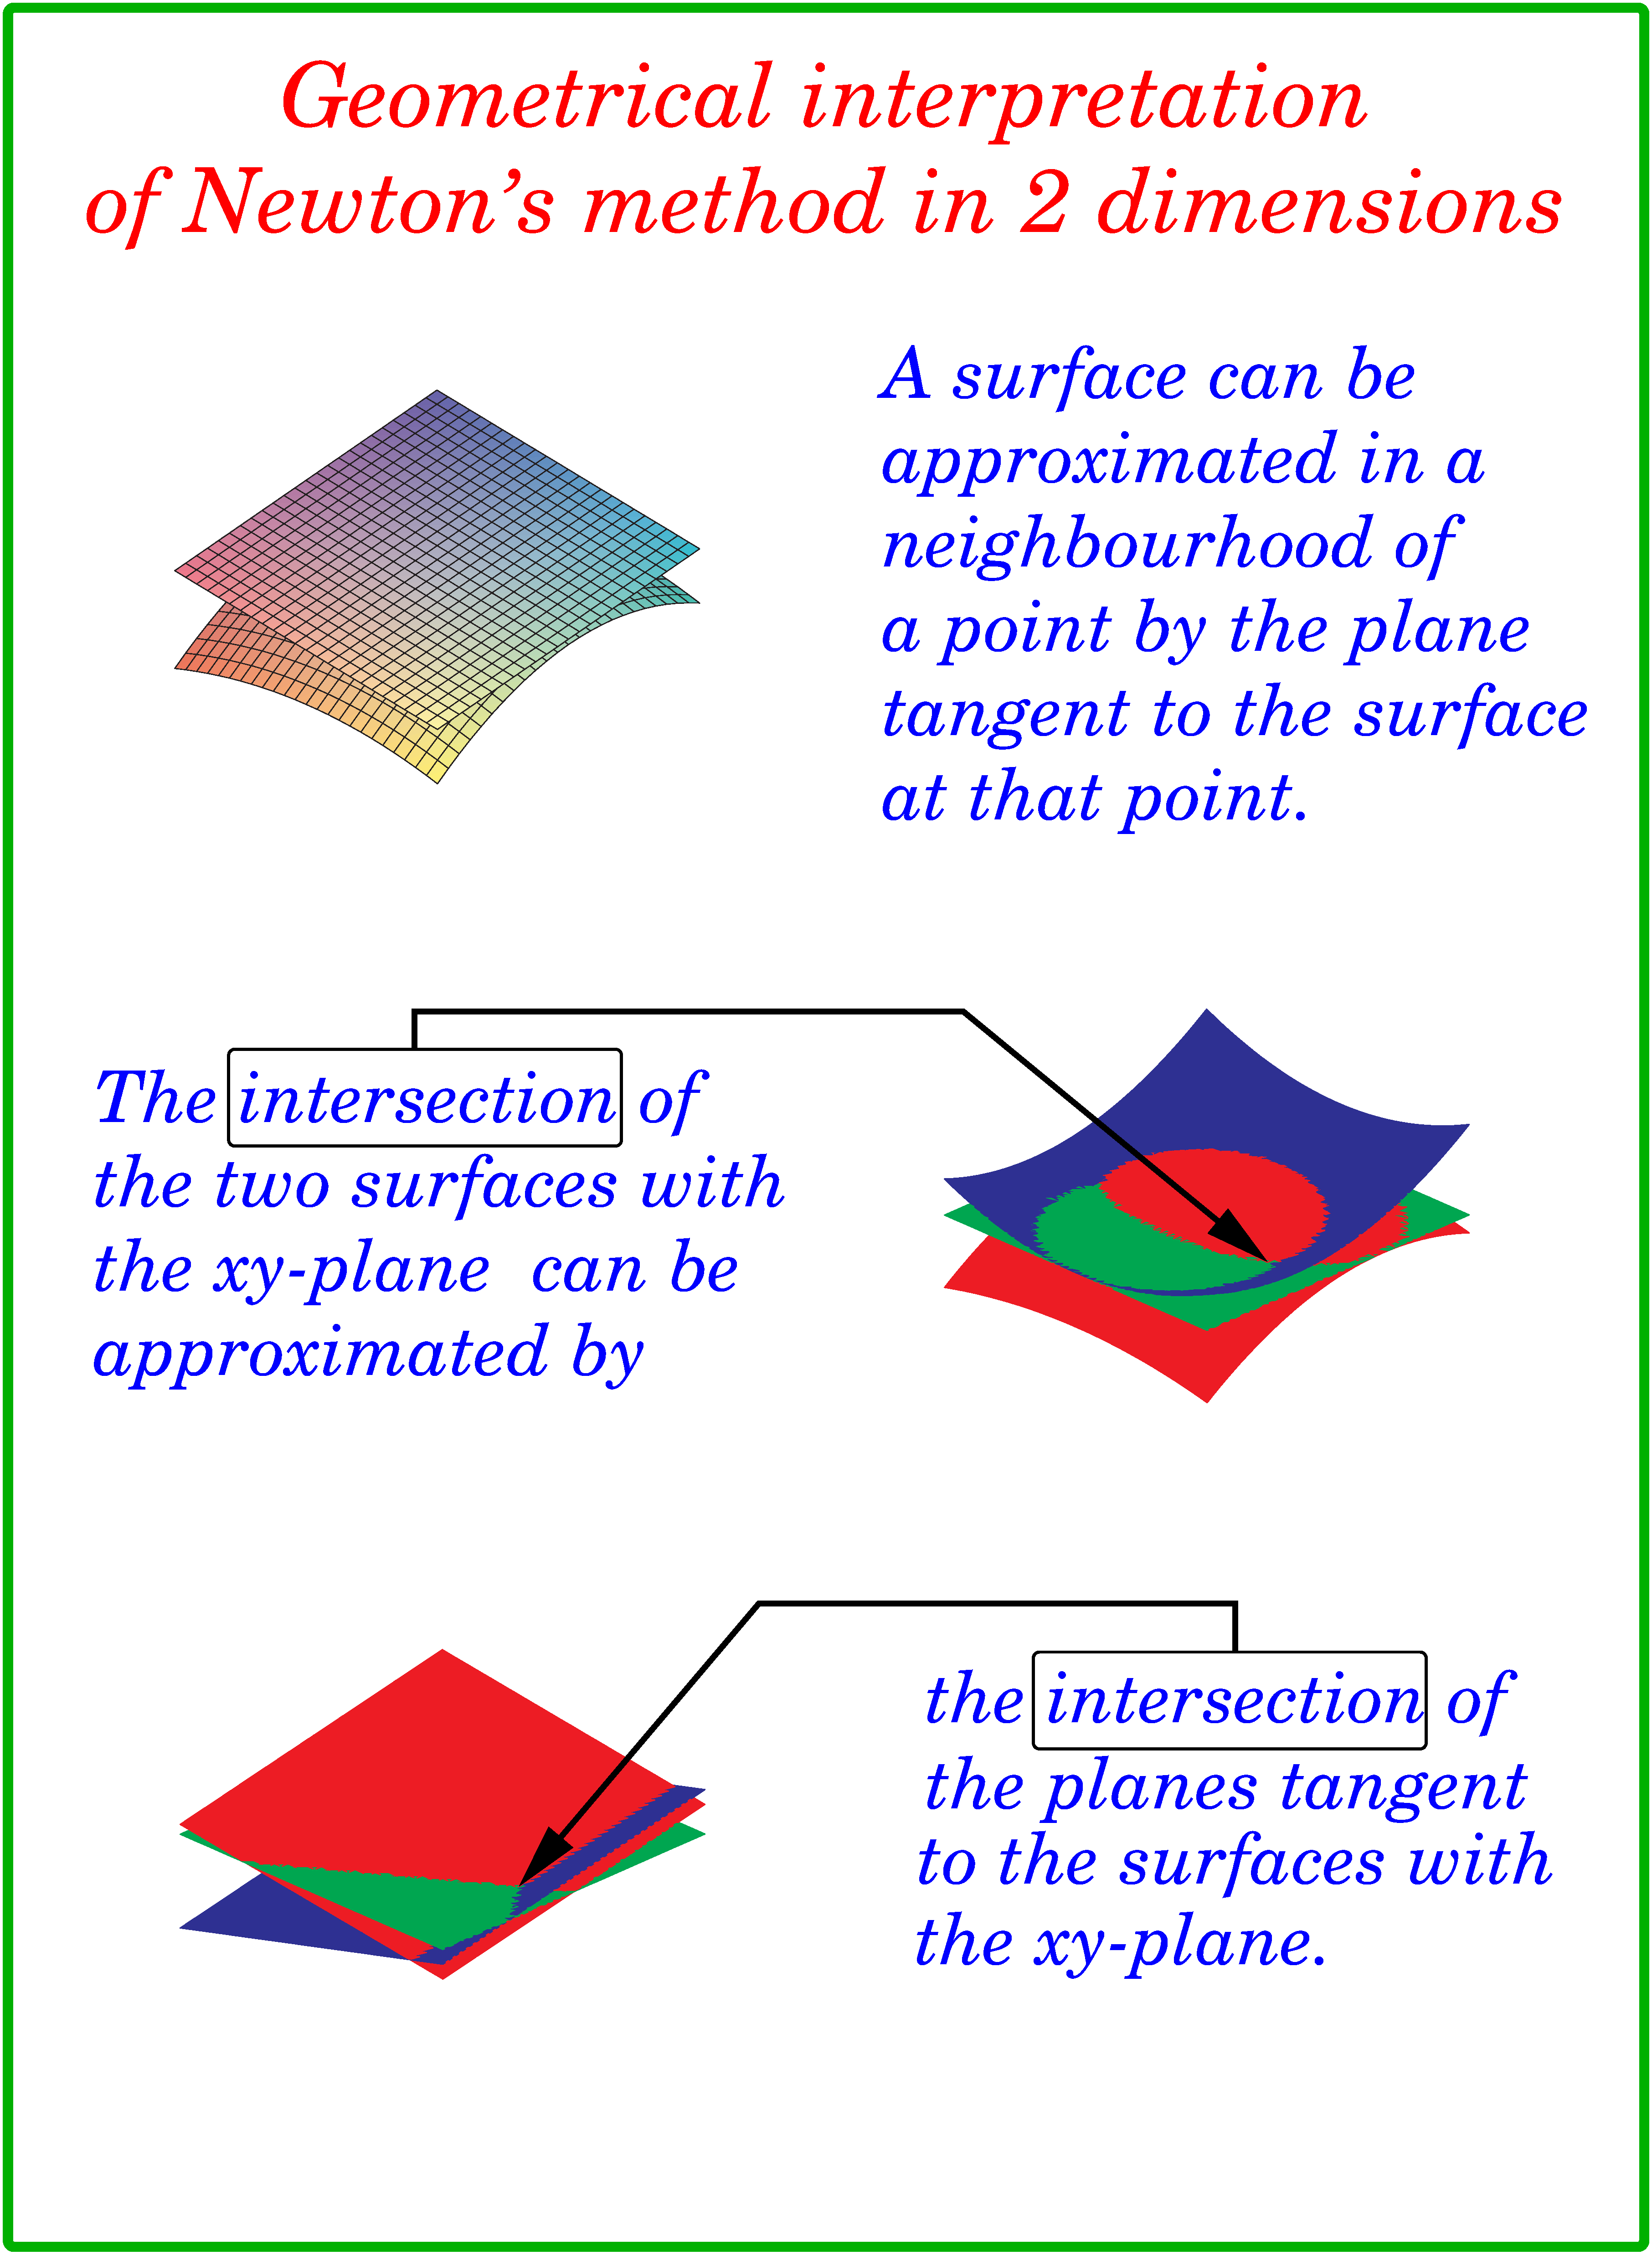
\includegraphics[width=150mm]{figures/Newt2}}
  \caption{\label{fig:Newt2} \it Geometrical meaning of Newton's
    method to solve a system of two nonlinear equations in two
    variables.  The solutions of the system are the intersections of
    the two surfaces with the $xy$-plane.}
\end{figure}

In discussing Newton's method we shall use only $2 \times 2$ systems,
but most of what we say generalises immediately to $n \times n$
systems.   The model problem that we wish to solve is
%
\begin{equation*}
  \begin{cases}
    f_1(x,y) = 0, \\ f_2(x,y) = 0 ,
  \end{cases}
  \quad \Longleftrightarrow \quad
  \bff(\bx) = 0 .
\end{equation*}
%
The easiest way to obtain an expression for Newton's method in two
dimensions is based on the its geometrical interpretation.   We start
by recapping the one dimension case: suppose that we wish to solve the
equation $f(x) = 0$ and that we have evaluated the function at $x_n$.
The next iterate, $x_{n+1}$ is the intersection of the straight line
tangent to the graph of $f(x)$ at $(x_n, f(x_n))$ with the $x$ axis.
The equation of this line is given by the first two terms of the
Taylor expansion of the function $f(x)$ around $x_n$:
%
\begin{equation*}
  y = f(x_n) + f'(x_n) (x - x_n) .
\end{equation*}
%
It intersects the $x$ axis at the point $x_{n+1}$ such that $y=0$, i.e.
%
\begin{equation*}
  0 = f(x_n) + f'(x_n) (x_{n+1} - x_n) \implies
  x_{n+1} =  x_n - \frac{f(x_n)}{f'(x_n)} .
\end{equation*}
%
The geometrical interpretation of Newton's method in two dimensions is
that the iterate $(x_{n+1},y_{n+1})$ is the common point where
the planes tangent to the graph of $f_1(x,y)$ and $f_2(x,y)$ at
$(x_n,y_n)$ intersect the $xy$-plane, i.e.\ the plane $z=0$ (see
Figure~\ref{fig:Newt2}).  The plane tangent to the two surfaces are
%
\begin{align*}
  z &= f_1(x_n,y_n) + (x - x_n) \pdv{f_1}{x}(x_n,y_n) +
  (y - y_n) \pdv{f_1}{y}(x_n,y_n) , \\
  z &= f_2(x_n,y_n) + (x - x_n) \pdv{f_2}{x}(x_n,y_n) +
           (y - y_n) \pdv{f_2}{y}(x_n,y_n) .
\end{align*}
%
At the intersection with the $xy$-plane we have $z=0$.
Therefore the equations for the next iterate are
%
\begin{align}
  f_1(x_n,y_n) + (x_{n+1} - x_n) \pdv{f_1}{x}(x_n,y_n) +
  (y_{n+1} - y_n) \pdv{f_1}{y}(x_n,y_n) &= 0 ,
  \label{eq:f1} \\
  f_2(x_n,y_n) + (x_{n+1} - x_n) \pdv{f_2}{x}(x_n,y_n) +
  (y_{n+1} - y_n) \pdv{f_2}{y}(x_n,y_n) &= 0 .
  \label{eq:f2}
\end{align}
%
We introduce the Jacobian of the function $\bff(\bx)$ at $(x_n,y_n)$,
%
\begin{equation*}
  J(x_n,y_n) =
  \begin{pmatrix}
    \partial_x f_1(x_n,y_n) & \partial_y f_1(x_n,y_n) \\
    \partial_x f_2(x_n,y_n) & \partial_y f_2(x_n,y_n)
  \end{pmatrix}
\end{equation*}
%
and write~(\ref{eq:f1}) and~(\ref{eq:f2}) in matrix notation as
%
\begin{equation*}
  J(x_n,y_n)
  \begin{pmatrix}
    x_{n+1} - x_n \\ y_{n+1} - y_n
  \end{pmatrix}
  =
  \begin{pmatrix}
    - f_1(x_n,y_n) \\ - f_2(x_n,y_n)
  \end{pmatrix}
  ,
\end{equation*}
%
so that the next iterate of Newton's method is
%
\begin{equation}
  \begin{pmatrix}
    x_{n+1} \\ y_{n+1}
  \end{pmatrix}
 =
 \begin{pmatrix}
   x_n \\ y_n
 \end{pmatrix}
 - J^{-1}
 \begin{pmatrix}
   -f_1(x_n,y_n) \\ -f_2(x_n,y_n)
 \end{pmatrix}
 . \label{Newtontwo}
\end{equation}
%
Equation~(\ref{Newtontwo}) generalises to $n$-dimensions as
%
\begin{equation}
  \bx_{n+1} = \bx_{n} -
  \left [ J(\bx_n) \right ]^{-1} \bff(\bx_n) . \label{NewtonRn}
\end{equation}
%
The scheme~(\ref{NewtonRn}) is numerically not convenient, because it
requires the computation of the inverse of the Jacobian.  Therefore,
one normally defines an additional variable
%
\begin{equation*}
  \bz = \bx_{n+1} - \bx_n \implies J \bz = - \bff(\bx_n) ,
\end{equation*}
%
and solves the linear problem for $\bz$ using, for example, Gauss
elimination with pivoting.  Once $\bz$ is known we can obtain
%
\begin{equation*}
  \bx_{n+1} = \bx_n + \bz .
\end{equation*}

\noindent
\textbf{Remark 1} - The initial guess is absolutely crucial and the
method can be very ``touchy''.  However, if we are close enough to the
root and the Jacobian is non singular the convergence is quadratic.

\noindent
\textbf{Remark 2} - Newton's method is very computationally intensive:
it requires the evaluation of $n^2$ derivatives and the solution of an
$n \times n$ linear problem at each iteration.  A multidimensional
version of the secant method has been developed to reduce the number
of computations per step (Broyden algorithm).


\section*{Further reading}

Topics covered here are also covered in
\begin{itemize}
\item Chapter 7 of Linz \& Wang, \textit{Exploring Numerical Methods}
  (QA297 LIN),
\item Chapter 3 of Kincaid \& Cheney, \textit{Numerical Analysis}
  (QA297 KIN),
\item Chapters 1 and 4 of S{\"u}li \& Mayers, \textit{An Introduction
    to Numerical Analysis} (not in library -- includes considerably
  more analysis of the convergence issues).
\end{itemize}


%\chapter{Interpolation}

\section{Introduction}

In numerical methods we often have a limited amount of information about a function, and we want to use that information to estimate, predict or compute additional quantities. For example, we may know (or be able to compute) the values of a function $f(x)$ at two points, say $x_1$ and $x_2$, and want to use this information to estimate the value of the function at a third point $x_3$.

This can be generalized to the idea of \emph{interpolation}. We assume, for example, that we know the value of a function at $N$ points $x_j$, with $j = 0, \dots, N-1$. We want to compute, or estimate, the value of the function at some other point $x$. This problem can be extended to multiple dimensions, or to vector functions component-by-component.

We will see later that interpolation is one way of approaching considerably more complicated problems. For example, we will typically perform interpolation by approximating the function that we are interested in (but do not know how to compute in general), $f$, with a different function $g$ that approximates $f$ (for example, equals $f$ at specific points) and that we can easily compute everywhere. We can then perform \emph{operations} on $g$, and treat them as giving approximately the same results as operations performed on $f$. For example, the integral of $f$ can be approximated by the integral of $g$.

\section{Polynomial interpolation}

We start with the one dimensional problem. We assume we do \emph{not} know anything about the function $f(x)$ except for its values $f_j \equiv f(x_j)$ at the \emph{nodes} $\{ x_j \}$, where $j = 0, \dots, N$. We want to interpolate $f$ to the general location $x$.

To do this we introduce an \emph{interpolating function} $g(x)$. The general form of the function $g$ will be given in advance: here it will be a polynomial,
%
\begin{align}
  g(x) &= c_0 + c_1 x + c_2 x^2 + \dots \\ &= \sum_k c_k x^k.
\end{align}
%
We will then fix the specific form -- that is, the range of the sum, and the value of the constants $\{ c_k \}$ -- by enforcing that $g(x_j) = f_j = f(x_j)$: i.e., the value of the interpolating function equals the value of the function being interpolated at the nodes. As we know $N+1$ pieces of information about the function $f$, we can fix $N+1$ coefficients of the polynomial $g$, meaning the sum should stop at $N$ (thanks to the $0$ power coefficient).

Therefore our interpolation problem becomes: given $f_j \equiv f(x_j)$ at the \emph{nodes} $\{ x_j \}$, where $j = 0, \dots, N$, find the coefficients $c_k$ such that the polynomial
%
\begin{equation}
  g(x) = \sum_{k=0}^{N} c_k x^k
\end{equation}
%
matches $f$ at the nodes, i.e., $f(x_j) = g(x_j)$.

We will use $g$ to interpolate, or approximate, $f$. Therefore we are also interested in the question of how accurately it does so: what is $g(x) - f(x)$?

\subsection{Lagrange polynomials}

The easiest polynomials to work with are the Lagrange basis polynomials. There are $N+1$ of these are polynomials, each of degree $N$, defined by their value at the nodes so that
%
\begin{equation}
  l^{(\ell)}(x_j) = \begin{cases} 1 & x_j = x_\ell \\ 0 & x_j \ne x_\ell \end{cases}.
\end{equation}
%
In words, the $\ell^{\text{th}}$ Lagrange basis polynomial has value $1$ at the $\ell^{\text{th}}$ node and vanishes at all other nodes. This immediately means that
%
\begin{equation}
  g(x) = \sum_{\ell=0}^{N} f(x_{\ell}) l^{(\ell)}(x)
\end{equation}
%
is \emph{an} interpolating polynomial: it is a polynomial of the right degree ($N$), and when evaluated at a node $x_j$ we have
%
\begin{align}
  g(x_j) &= \sum_{\ell=0}^{N-1} f(x_{\ell}) l^{(\ell)}(x) \\
  &= f_{j}
\end{align}
%
as all the basis functions vanish at all the nodes \emph{except} for the $j^{\text{th}}$ one which has value $1$.

Now that we know that the Lagrange basis functions $l^{(\ell)}(x)$ are what we want, we need an explicit way of constructing them. We know that they must be polynomials, so we can write them as products of the form $(x - a)$. We know that we want them to vanish at all the nodes (except one), so the obvious form of these individual terms would be $(x - x_j)$. Finally, we konw that at the $\ell^{th}$ node we do not want them to vanish (so there should be so term of the form $(x - x_\ell)$), but instead want the value to be one. This gives us the value of the overall scaling constant. From these considerations we see that
%
\begin{equation}
  l^{(\ell)}(x) = \prod_{m=0, m \ne \ell}^{N} \frac{x - x_m}{x_{\ell} - x_m}.
\end{equation}

\subsection{Low order examples}

Putting everything together we have that $f(x) \simeq g(x)$, where the Lagrange polynomial interpolating function is given by
%
\begin{equation}
  g(x) = \sum_{j=0}^{N-1} f(x_{j}) \prod_{m=0, m \ne j}^{N-1} \frac{x - x_m}{x_j - x_m}.
\end{equation}
%
We can explicitly check the simple examples.

\subsubsection{Linear interpolation}

To get a linear interpolating polynomial we need the interpolating polynomial to have two coefficients (the constant and the linear part), meaning we need $N=1$. Therefore we are assuming we know $f(x)$ at the two nodes $x_0$ and $x_1$.

The Lagrange basis polynomials are
%
\begin{align}
  l^{(0)}(x) &= \frac{x - x_1}{x_0 - x_1}, \\
  l^{(1)}(x) &= \frac{x - x_0}{x_1 - x_0}.
\end{align}
%
This gives the interpolating polynomial as
%
\begin{align}
  g(x) &= f(x_0) \frac{x - x_1}{x_0 - x_1} + f(x_1) \frac{x - x_0}{x_1 - x_0}, \\
  &= f(x_0) \left( 1 - \frac{x - x_0}{x_1 - x_0} \right) + f(x_1) \frac{x - x_0}{x_1 - x_0}.
\end{align}
%
The final form of the equation can be written as $g(x) = f_0 (1 - \Delta) + f_1 \Delta$, where $\Delta$ is the distance between $x$ and $x_0$ relative to the distance between $x$ and $x_1$.

\subsubsection{Quadratic interpolation}

For quadratic interpolation we have $N=2$, which requires assuming knowledge of $f(x)$ at $x_0, x_1$ and $x_2$. The Lagrange basis polynomials are
%
\begin{align}
  l^{(0)}(x) &= \frac{(x - x_1)(x - x_2)}{(x_0 - x_1)(x_0 - x_2)}, \\
  l^{(1)}(x) &= \frac{(x - x_0)(x - x_2)}{(x_1 - x_0)(x_1 - x_2)}, \\
  l^{(2)}(x) &= \frac{(x - x_0)(x - x_1)}{(x_2 - x_0)(x_2 - x_1)}.
\end{align}
%
This gives the interpolating polynomial as
%
\begin{align}
  g(x) &= f(x_0) \frac{(x - x_1)(x - x_2)}{(x_0 - x_1)(x_0 - x_2)} + f(x_1) \frac{(x - x_0)(x - x_2)}{(x_1 - x_0)(x_1 - x_2)} + f(x_2) \frac{(x - x_0)(x - x_1)}{(x_2 - x_0)(x_2 - x_1)}.
\end{align}
%
In the special case where the points are equally spaced, $x_1 - x_0 = h = x_2 - x_1$, implying that $x_2 - x_0 = 2 h$, and using the coordinate $\hat{x} = x - x_1$, we get
%
\begin{equation}
  g(x) = \frac{1}{2 h^2} \left( f_0 \hat{x} (\hat{x} - h) - 2 f_1 (\hat{x} + h) (\hat{x} - h) + f_2 (\hat{x} + h) \hat{x} \right).
\end{equation}
%
This particular form is useful for integration and differentiation. For example,
%
\begin{align}
  \eval{\dv{g}{x}}_{x = x_1} &= \eval{\dv{g}{x}}_{\hat{x} = 0} \\
  &= \left. \frac{1}{2 h^2} \left( f_0 (2 \hat{x} - h) - 2 f_1 (2 \hat{x}) + f_2 (2 \hat{x} + h) \right) \right|_{\hat{x} = 0} \\
  &= \frac{1}{2 h} \left( f_2 - f_0 \right).
\end{align}

\section{Accuracy}

We want to know how close the interpolating polynomial $g(x)$ gets to the function $f$ that it is interpolating: that is, we want to know the size of the error $e(x) = f(x) - g(x)$. As $f$ is completely general, we will never know this exactly: however, we can make some general points.

First, we have explicitly chosen $g$ such that it agrees with $f$ at all of the nodes. That means the error must have the form
%
\begin{equation}
  e(x) = f(x) - g(x) = F(x) \prod_{j=0}^N (x - x_j).
\end{equation}
%
That is, the error function vanishes at the nodes, $e(x_j) \equiv 0$.

Second, we note that at any fixed point $X$, we can use a Taylor series expansion that matches the terms in the polynomial $g$. That is (under some assumptions), there is a value $\xi$ such that
%
\begin{equation}
  e(X) = f(X) - g(X) = \frac{1}{(N+1)!} \eval{\dv[N+1]{f}{x}}_{x=\xi} \prod_{j=0}^N (X - x_j).
\end{equation}
%
The precise form matters less than the interpretation. The important point is that the error depends on (a) the magnitude of the derivative of the function being interpolated, and (b) the magnitude of the product $\prod_{j=0}^N (x - x_j)$. The first cannot be controlled except by changing $N$. The second can be controlled both by changing $N$ and by changing the location of the nodes.

We focus on the term $|\prod_{j=0}^N (x - x_j)|$. If we make the nodes equally spaced then each term $x - x_j \propto h$, where $h = x_{j+1} - x_j$. This means the error is $e(x) \propto h^{N+1}$ and we expect the error to decay rapidly if $h$ is sufficiently small. In particular this implies that the larger $N$ is, the faster the error will decay as we make $h$ smaller. Whilst this is usually true, by ignoring the other terms in the error we may be ignoring larger errors, and even ones that grow: the Runge phenomenon is one example of this.

We also note (without proof!) that we can reduce the error by \emph{not} choosing the nodes to be equally spaced. For example, if we restrict the nodes to lie within $(-1, 1)$, by choosing the Chebyshev nodes
%
\begin{equation}
  x_j = \cos \left( \frac{2 j + 1}{2 (N + 1)}) \pi \right)
\end{equation}
%
the error $e(x)$ will behave as $e(x) \propto 2^{-N} / N!$. Using appropriate non-equally spaced nodes is often better in terms of accuracy, but may be more work to set up for integration and differentiation.


\chapter[Quadrature]{Numerical Quadrature}

\section{Introduction}

There are many circumstances in mathematical modelling when we need to
evaluate an integral, like
%
\begin{equation}
 \mint{a}{b}{f(x)}{x} .\label{Qua:eq:1}
\end{equation}
%
However, the integrals that can be evaluated analytically are few and
many integrals of great interest in engineering, like, for example,
the error function,
%
\begin{equation}
 \mbox{Erf}(x) = \mint{-\infty}{x}{e^{-\xi^2}}{\xi} \label{Qua:eq:2}
\end{equation}
%
can only be evaluated numerically.

We discuss two major techniques to evaluate integrals
(\textit{quadrature}): the first is based on \textit{interpolation},
the second on \textit{Gaussian quadrature}.

\section{Polynomial interpolation}

If we want to work with any function $f(x)$ numerically we must expect
to represent it using a finite amount of information. Typically this
is done by assuming that we know only the value of the function at a
finite set of points, call \textit{nodes}, $\{x_j\}$, with
$j=0,\ldots,N$. We denote the function values $f_j \equiv f(x_j)$.

One standard approach is to approximate the function $f$ by another
function $g(x)$ which is easy to manipulate and \textit{interpolates}
$f$ at the nodes, i.e.
%
\begin{equation}
  g(x_j) = f_j = f(x_j), \quad j = 0, \ldots, N.
\end{equation}
%
We then use $g$ in place of $f$ wherever necessary, as we shall see
below.

One standard, simple choice of \textit{interpolating function} $g(x)$
is a polynomial. Given the $N+1$ values $f_j$ at the nodes $x_j$ there
is a \emph{unique} polynomial $g$ of order $N$ that interpolates $f$
(as should be clear, as a polynomial of order $N$ has $N+1$
coefficients to be fixed). There are two standard forms of writing
this polynomial explicitly. Here we just show the Lagrange form to
show the explicit construction is possible. Often the Newton form is
used in numerical calculations instead.

First, given the nodes $x_j$, define the \textit{fundamental
  polynomials} $\ell_j(x)$ by
%
\begin{equation}
  \ell_j(x) = \prod_{\substack{i = 0\\i \ne j}}^N \frac{x - x_i}{x_j -
    x_i}, \quad j = 0, 1, \dots, N.
\end{equation}
%
These have the property that $\ell_j(x_j) = 1$ and $\ell_j(x_k) = 0, j
\ne k$. It follows that
%
\begin{equation}
  g(x) = \sum_{j=0}^N f(x_j) \ell_j(x)
\end{equation}
%
is the polynomial of degree $N$ that interpolates the function $f(x)$
at the nodes $x_j$.

In what follows we shall see methods for solving quadrature and
differential equations based on polynomial interpolation. For these
the defining features are the locations of the nodes and the order of
the interpolating polynomial. In many cases the formulas will simplify
greatly from the general Lagrange form above, so each case is treated
separately.

\section[Using polynomial interpolation]{Numerical integration based on polynomial interpolation}

\subsection{Introduction}

We assume that we can evaluate the function at a finite set of points,
called \textit{nodes}, $\{x_j\}$, with $j=0,\ldots, N$ in the interval
$[a,b]$ and we want to estimate~(\ref{Qua:eq:1}).  The idea behind all
the methods based on polynomial interpolation is that we can replace
the function $f(x)$ with a simpler function $g(x)$, i.e.\ a function
whose integral we can evaluate analytically.  We require that the
function $g(x)$ \textit{interpolates} the function $f(x)$, i.e.\ that
it has the same value as $f(x)$ at the nodes:
%
\begin{equation}
  g(x_j) = f(x_j) , \qquad j = 0,1,\ldots,N. \label{Qua:eq:3}
\end{equation}
%
The simplest choice of class of functions $g(x)$ are polynomials and
the different quadrature interpolation methods are differentiated by
the order of the polynomial interpolation.  Formulae based on
polynomial interpolation with equally spaced nodes go under the
generic name of \textit{Newton-Cotes formulae}.

\subsection{Trapezoidal rule}

\begin{figure}
  \centerline{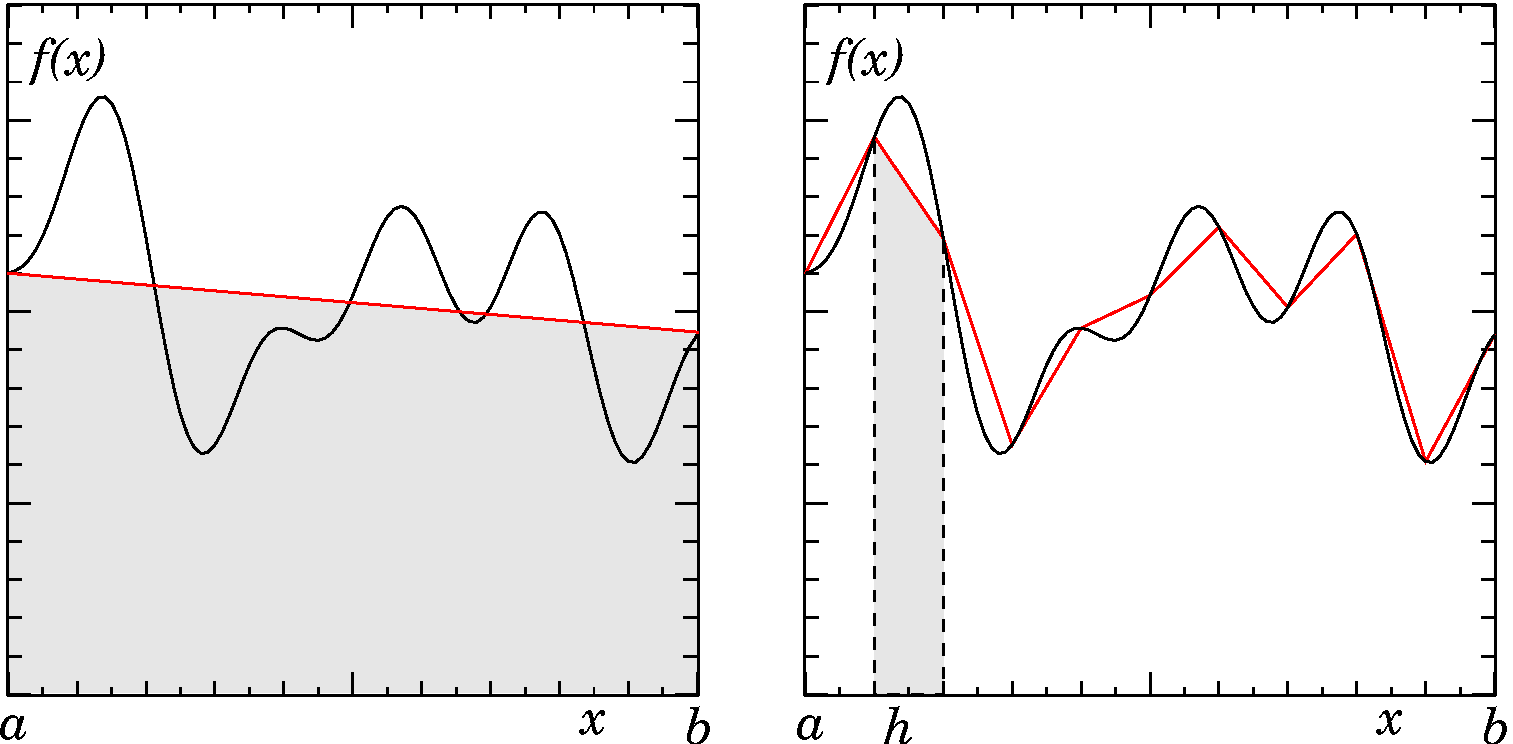
\includegraphics[width=135mm]{figures/trapez}}
  \caption{\label{fig:trapez} \it The trapezoidal rule is based on the
    approximation of the given function $f(x)$ with an order one
    polynomial (left).  In general one uses a composite trapezoidal
    rule: the integration range is divided in intervals of length $h$
    and the function is approximated by a different polynomial on each
    interval (right).}
\end{figure}

The simplest case results if we choose an interpolating polynomial of
order one, i.e.\ we replace the function with a straight line that
interpolates the function at the end points of the integration range
(see left panel of Figure~\ref{fig:trapez}).   The area under the line
is given by
%
\begin{equation}
  A = \frac{1}{2} (b-a) [f(a) + f(b)]
  \label{Qua:eq:32}
\end{equation}
%
and this is the approximate value of~(\ref{Qua:eq:1}) according to the
\textit{trapezoidal rule}.  It is clear that unless the range $[a,b]$
is very small the error in the estimate obtained using the trapezoidal
rule is very large.  The standard procedure is to make use of the
\textit{composite trapezoidal rule}: the integration range is divided
into $N$ intervals of length $h$ and the function $f(x)$ is
approximated on each interval by a straight line that interpolates the
function at the nodes (see right panel of Figure~\ref{fig:trapez}).
The area under each segment of the piecewise linear curve is
%
\begin{equation}
  A_j = \frac{1}{2} (x_{j}-x_{j-1}) [f(x_{j})+f(x_{j-1})] , \quad
  j = 1,2, \ldots, N.
  \label{Qua:eq:4}
\end{equation}
%
By summing all the areas we obtain the composite trapezoidal rule:
%
\begin{equation}
  \mint{a}{b}{f(x)}{x} = \sum_{j=1}^{N} A_j =
  \frac{1}{2} \sum_{j=1}^{N} (x_{j}-x_{j-1}) [f(x_{j})+f(x_{j-1})]
  \label{Qua:eq:5}
\end{equation}
%
If the nodes are equally spaced, i.e.\ if $(x_{j}-x_{j-1}) = h$ for all
$j=1, \ldots, N$, this formula reduces to:
%
\begin{equation}
 \mint{a}{b}{f(x)}{x} =
  \frac{h}{2} \sum_{j=1}^{N} [f(x_{j})+f(x_{j-1})] =
  \frac{h}{2} ( f_0 + 2 f_1 + 2 f_2 + \ldots + 2 f_{N-1} + f_N ) ,
\label{Qua:eq:12}
\end{equation}
%
where $f_j \equiv f(x_j)$.  The error in the approximation is given by
%
\begin{equation}
  \text{Error} \le \frac{1}{12} h^3 N M_2 =
  \frac{(b-a) h^2}{12} M_2 , \qquad
  M_2 = \max_{x\in[a,b]} |f''(x)| .
  \label{Qua:eq:6}
\end{equation}

\subsection{Simpson's rule}

\begin{figure}
  \centerline{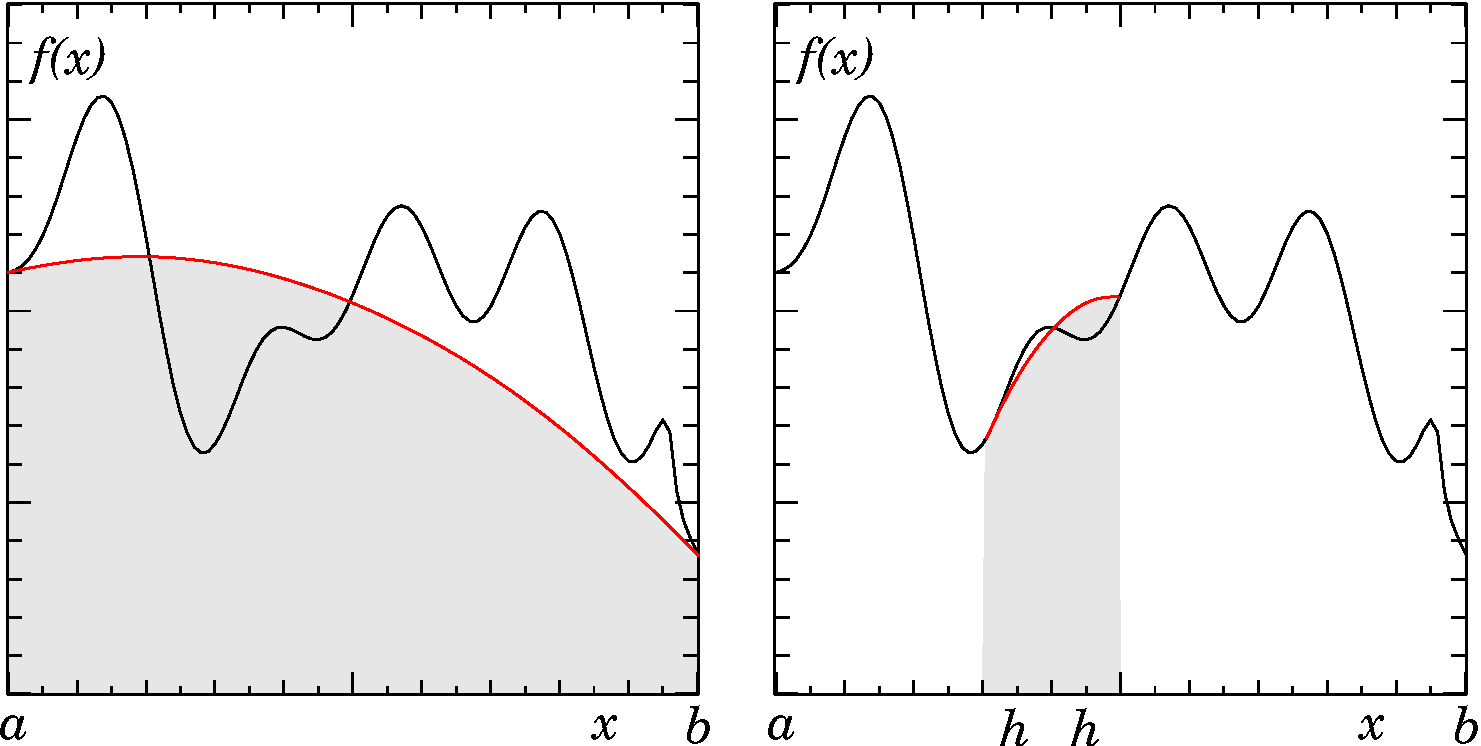
\includegraphics[width=135mm]{figures/simpson}}
  \caption{\label{fig:simpson} \it Simpson's rule is based on the
    approximation of the given function $f(x)$ with an order two
    polynomial (left).  In general one uses a composite Simpson's
    rule: the integration range is divided in intervals of length $2
    h$ and the function is approximated by different parabolas on each
    interval.}
\end{figure}

In this case the function is approximated with a polynomial of order
two (a parabola, see left panel of Figure~\ref{fig:simpson}).  We can
obtain the formula for the quadrature by writing the interpolating
polynomial and integrating it.  It turns out that the area under the
parabola is given by
%
\begin{equation}
  A = \frac{b-a}{6}
  \left [ f(a) + 4 f\left(\frac{a+b}{2}\right) + f(b) \right ],
  \label{Qua:eq:33}
\end{equation}
%
and this is the approximate value of~(\ref{Qua:eq:1}) according to
\textit{Simpson's rule}.  It is clear that unless the range $[a,b]$ is
very small the error in the estimate obtained using the trapezoidal
rule is very large.  The standard procedure is to make use of the
\textit{composite Simpson's rule}: the integration range is divided
into $N/2$ intervals of length $2 h$, with $N$ an even number. The
function $f(x)$ is approximated on each interval by a parabola that
interpolates the function at the nodes (see right panel of
Figure~\ref{fig:simpson}).  For simplicity we assume that the
interpolation points $\{x_j\}$, $j=0,1,2,\ldots,N$ are all equally
spaced so that we can write:
%
\begin{equation*}
  x_j = x_0 + j h .
\end{equation*}
%
The area under the parabola joining the nodes $x_{j-1}$, $x_{j}$ and
$x_{j+1}$ is
%
\begin{equation}
  A_j = \frac{h}{3} \left[f(x_{j-1})+4f(x_{j})+f(x_{j+1})\right]
  \label{Qua:eq:9}
\end{equation}
%
where $j=1,3,5,\ldots, N-1$.  This result is known as
\textit{Simpson's rule}.  If we apply it to all the sub-intervals in
$[a,b]$ we obtain the composite Simpson rule:
%
\begin{equation}
  \mint{a}{b}{f(x)}{x} = \sum_{k=1}^{N/2} A_{2k-1} =
  \frac{h}{3} \left[ f(a) +
    2 \sum_{j=1}^{N/2-1} f(x_{2j}) +
    4 \sum_{j=1}^{N/2} f(x_{2j-1}) + f(b) \right] + R,
  \label{Qua:eq:10}
\end{equation}
%
where the estimate for the error is given by
%
\begin{equation}
  |R|\le \frac{M_4}{180}(b-a)h^4,\label{Qua:eq:11}
\end{equation}
%
where $M_4=\max|f^{(4)}(x)|$ with $a \le x \le b$.  Note that
Simpson's rule is exact for any cubic polynomial as $f^{(4)}(x) \equiv
0$ for all polynomials of order three.

We can obtain an estimate of the error by proceeding as follows.  We
compare the Taylor expansion of Simpson's rule for the integral in the
range $[x_{j-1},x_{j+1}]$, given by equation~(\ref{Qua:eq:9}), to the
Taylor expansion of the exact integral.  The error is the first term
in the difference of the two Taylor expansions.  We start with the
Taylor expansion of the Simpson's rule estimate of
%
\begin{equation}
  \mint{x_{j-1}}{x_{j+1}}{f(x)}{x} \simeq A_j =
  \frac{h}{3} [ f(x_{j-1}) + 4 f(x_{j}) + f(x_{j+1}) ] ,
  \label{Qua:eq:19}
\end{equation}
%
where, to simplify the notation, we use the notation $f_j=f(x_j)$,
$f'_j=f'(x_j)$, and, in general, $f^{(n)}_j$ for the $n$-th derivative
of $f(x)$ evaluated at $x=x_j$.  Using Taylor's theorem to expand
$f(x)$ at $x=x_j$ we can write
%
\begin{equation}
  A_j = 2 h f_j + \frac{h^3}{3} f_j'' + \frac{h^5}{36} f_j^{(4)} + \order{h^6}
  \label{Qua:eq:20}
\end{equation}
%
We now need to compute the Taylor expansion in powers of $h$ of the
exact result.  In order to do this we introduce the function
%
\begin{equation}
  F(t) = \mint{x_j-t}{x_j+t}{f(x)}{x} .
  \label{Qua:eq:21}
\end{equation}
%
Note that with this notation
%
\begin{equation}
  \mint{x_{j-1}}{x_{j+1}}{f(x)}{x} = F(h).
  \label{Qua:eq:14}
\end{equation}
%
Therefore, in order to compute the Taylor expansion in powers of $h$
of the exact result of the integral in equation~(\ref{Qua:eq:14}), we
need to expand $F(t)$ in Taylor series around $t=0$:
%
\begin{equation}
  F(h) = F(0) +
  h \eval{\dv{F}{t}}_{t=0}  +
  \frac{h^2}{2} \, \eval{\dv[2]{F}{t}}_{t=0}  +
  \ldots +
  \frac{h^5}{5!} \, \eval{\dv[5]{F}{t}}_{t=0} +
  \order{h^6}
  \label{Qua:eq:15}
\end{equation}
%
We note that $F(0)=0$.  Moreover, by the fundamental theorem of
calculus (with a little help from the chain rule)
%
\begin{equation*}
  \dv{F}{t} = f(x_j+t) + f(x_j-t) \implies
  \dv[n]{F}{d} = f^{(n-1)}(x_j+t) +
  (-1)^{n+1} f^{(n-1)}(x_j-t) .
\end{equation*}
%
Note that all the even derivatives of $F(t)$ are zero at $t=0$ so that
the Taylor expansion of~(\ref{Qua:eq:15}) becomes
%
\begin{equation}
  2 h f_j + \frac{h^3}{3} f_j'' + \frac{h^5}{60} f_j^{(4)} + \order{h^6}.
  \label{Qua:eq:30}
\end{equation}
%
Combining these two expansions, we have that the local error in the
interval $[x_{j-1},x_{j+1}]$ is, up to order $h^6$,
%
\begin{equation}
  E_j \equiv F(h) - A_j = - \frac{1}{90} h^5 f_j^{(4)} \implies
  \abs{E_j} \le \frac{1}{90} h^5 M_4 ,
  \label{Qua:eq:31}
\end{equation}
%
where $M_4$ is the same as in equation~(\ref{Qua:eq:11}).  Summing the
local errors over all the intervals used in the composite Simpson's
rule gives the total error, $R$,
%
\begin{equation}
  \abs{R} = \abs{\sum_{k=1}^{N/2} E_{2k-1}} \le
  \sum_{k=1}^{N/2} \abs{ E_{2k-1} } \le
  \sum_{k=1}^{N/2} \frac{1}{90} h^5 M_4 = \frac{M_4}{180}(b-a)h^4.
\end{equation}

\subsection{Richardson extrapolation}

This is a very general technique that uses the information on the rate
of decrease of the error to get a better estimate of the numerical
result required.  As such it can be applied to many different
algorithms, not just quadratures.  However, here we illustrate it in
the context of Simpson's rule.

Equation~(\ref{Qua:eq:11}) tells us that the error on the estimate of
the integral decreases with the fourth power of the integration step,
$h$.  However, in order to estimate the error using this formula we
would also need the value of the coefficient $M_4$.  We can get round
this problem by using the following procedure.  Indicate with $I_n$
the estimate of the integral using $n$ intervals and with $I$ the
exact value of the integral.  From~(\ref{Qua:eq:11}) we have that
%
\begin{equation}
  I - I_{2n} \simeq C (2n)^{-4} =
  2^{-4} \left ( C n^{-4} \right ) \simeq 2^{-4} (I - I_n) .
  \label{Qua:eq:16}
\end{equation}
%
In this last step we have assumed that the constant $C$ is the same
whether we use $n$ or $2n$ intervals to estimate the integral.  This
not strictly true, but it is a reasonable approximation if the
integration range is small enough.  From~(\ref{Qua:eq:16}) we have
that the exact value of the integral is approximately
%
\begin{equation*}
  I \simeq \frac{2^4 I_{2 n} - I_n}{2^4 -1}
\end{equation*}
%
and we use this as the new estimate of the integral
(\textit{Richardson extrapolated value}):
%
\begin{equation}
  R_{2 n} = \frac{2^4 I_{2 n} - I_n}{2^4 -1} .
  \label{Qua:eq:22}
\end{equation}
%
The error in the approximation is roughly
%
\begin{equation}
  E_{2n} \equiv \abs{ R_{2 n} - I_{2 n} } = \frac{\abs{I_n - I_{2 n}}}{2^4 -1} .
  \label{Qua:eq:17}
\end{equation}
%
This quantity is called the \textit{computable estimate of the error}.

\subsection{Adaptive quadrature}

Adaptive quadrature methods are intended to compute definite integrals
to a given precision by automatically choosing a set of nodes that
takes into account the behaviour of the integrand by being denser
where the integrand varies more rapidly. Ideally, the user supplies
only the integrand $f$, the interval $[a,b]$, and the accuracy
$\epsilon$ desired for computing the integral
%
\begin{equation}
  \mint{a}{b}{f(x)}{x} . \label{Qua:eq:23}
\end{equation}
%
The program then divides the interval into sub-intervals of varying
length so that numerical integration on these sub-intervals will
produce results of acceptable precision. The main idea is that if
Simpson's rule on a given sub-interval is not sufficiently accurate,
that interval will be divided into two equal parts, and Simpson's rule
will be used on each half. This procedure will be repeated in an
effort to obtain an approximation to the integral with the same
accuracy over all the sub-intervals involved.  A rough algorithm is as
follows:

\begin{enumerate}
  %
\item Compute the integral~(\ref{Qua:eq:23}) using $3$ points and
  estimate the global error.  If the error is smaller than the
  tolerance stop.
  %
\item Divide the interval into two equal parts.  Consider each part in
  turn.
  %
\item Compute the integral on the sub-interval using $3$ points,
  i.e.\ using a finer grid.
%
\item Estimate the error on the evaluation of the integral over the
  sub-interval.  If it is larger than the maximum acceptable local
  error then divide the sub-interval in two and start again from point
  (2).  Otherwise go to point (3) and work on the next sub-interval if
  there are any left.
%
\end{enumerate}

In order to apply this idea we need to firstly to estimate the
\textit{local error}: we can do this using Richardson's extrapolation
and equation~(\ref{Qua:eq:17}).  Secondly, we need to estimate the
\textit{global error} on the integration over the entire interval
$[a,b]$ as a function of the local errors.

\smallskip

\noindent
We indicate with $e_i$ the local error on the integration over the
segment $[x_{i-1},x_i]$. If
%
\begin{equation}
  \abs{e_i} \le \epsilon (x_i-x_{i-1})/(b-a),
  \label{Qua:eq:25}
\end{equation}
%
then the total error will be bounded by
%
\begin{equation}
  \abs{ \sum_{i=1}^n e_i} \le \sum_{i=1}^n \abs{e_i} \le
  \frac{\epsilon}{b-a} \sum_{i=1}^n (x_i-x_{i-1}) = \epsilon.
  \label{Qua:eq:26}
\end{equation}
%
Therefore in the adaptive quadrature algorithm outlined above we have
to ensure that the local error satisfies~(\ref{Qua:eq:25}).

\section{Gaussian Quadrature}

The aim of all quadrature techniques is to create formulae of the type
%
\begin{equation}
  \mint{a}{b}{f(x)}{x} \simeq \sum_{i=1}^n w_i f(x_i) .
 \label{Qua:eq:18}
\end{equation}
%
In the trapezoidal and Simpson's rule the points where the function is
evaluated, $x_i$, are fixed \textit{a priori} and we obtain
that~(\ref{Qua:eq:18}) is exact for all polynomial of degree less than
or equal to $n$.  In the case of the trapezoidal rule we have $n=2$
and the rule is exact for all linear functions.  In the case of
Simpson's rule we have $n=3$ and we would expect the formula to be
exact for all quadratic polynomials.  As a matter of fact, it is exact
for polynomials of order three, but this is due to a happy
cancellation.

However, there is no obligation to fix the nodes.  As a matter of fact
we could fix the coefficients (called \textit{weights}) $w_i$, for
example set them all to one, or we could not fix anything.  The
general criterion to find nodes and weights is to require that
equation~(\ref{Qua:eq:18}) is as accurate as possible, i.e.\ that it is
exact for polynomials of degree as high as possible.  In other words,
we require that the nodes and weights are such that
%
\begin{equation}
  \mint{a}{b}{x^s}{x} = \sum_{i=1}^n w_i x_i^s, \quad s=0,1,...,N,
  \label{Qua:eq:27}
\end{equation}
%
with $N$ as large as possible.

As above, we define the \textit{fundamental polynomials}
$\ell_i(x)$ given by
%
\begin{equation}
  \ell_i(x) = \prod_{\substack{j = 0\\j \ne i}}^N \frac{x - x_j}{x_i -
    x_j}, \quad i = 0, 1, \dots, N,
\end{equation}
%
have the property that $\ell_i(x_i) = 1$ and $\ell_i(x_k) = 0, i \ne
k$. It follows that
%
\begin{equation}
  p(x) = \sum_{i=0}^N f(x_i) \ell_i(x)
\end{equation}
%
is the polynomial of degree $N$ that interpolates the arbitrary
function $f(x)$ at the given nodes $x_i$. If the nodes are known or
fixed we can therefore immediately compute the weights as
%
\begin{equation}
  w_i = \mint{a}{b}{\ell_i(x)}{x}.
\end{equation}
%

If neither the nodes nor the weights are fixed we have $N$ nonlinear
equations for $2n$ unknowns $x_1,...,x_n$ and $w_1,...,w_n$.  One can
show that this problem has a unique solution if $N=2n-1$, i.e.\ that it
is possible to compute exactly the integrals of polynomials of degree
up to $2 n - 1$.  The resulting algorithm is called a {\bf Gaussian
  quadrature}.  There are many formulae for Gaussian quadrature that
depend mainly on the choice of integration interval and on the type of
the integral.  A generic Gauss quadrature formula is
%
\begin{equation}
  \mint{a}{b}{W(x) f(x)}{x} = \sum_{i=1}^n w_i f(x_i)
\end{equation}
%
and the different formulae are summarised in the following table:

\begin{center}
 \begin{tabular}{lll} \hline
  $(a,b)$ & $W(x)$ & Gauss- \\ \hline
  $(-1,1)$ & 1 & Legendre \\
  $(-1,1)$ & $(1-x^2)^{-1/2}$ & Chebychev \\
  $(0,\infty)$ & $x^c e^{-x}$ & Laguerre $c=0,1,\ldots$ \\
  $(-\infty,+\infty)$ & $e^{-x^2}$ & Hermite \\ \hline
 \end{tabular}
\end{center}

\section*{Further reading}

Topics covered here are also covered in
\begin{itemize}
\item Chapter 6 of Linz \& Wang, \textit{Exploring Numerical
    Methods} (QA297 LIN),
\item Chapter 7 of Kincaid \& Cheney, \textit{Numerical Analysis}
  (QA297 KIN),
\item Chapters 7 and 10 of S{\"u}li \& Mayers, \textit{An Introduction
    to Numerical Analysis} (not in library).
\end{itemize}

The issue of representing an arbitrary function by an interpolating
function, which will recur in later chapters, is covered in
considerable detail elsewhere; for example\begin{itemize}
\item Chapters 4 and 5 of Linz \& Wang, \textit{Exploring Numerical
    Methods} (QA297 LIN),
\item Chapter 6 of Kincaid \& Cheney, \textit{Numerical Analysis}
  (QA297 KIN),
\item Chapters 6, 8, 9 and 11 of S{\"u}li \& Mayers, \textit{An Introduction
    to Numerical Analysis} (not in library).
\end{itemize}


\chapter[Initial value problems]{Initial value problems for Ordinary Differential Equations}

\section{Introduction}

A system of first order differential equation (ODE) is a relationship
between an unknown (vectorial) function $\by(x)$ and its derivative
$\by'(x)$. The general system of first order differential equations
has the form
%
\begin{equation}
  \by'(x)=\boldsymbol{f}(x,\by(x)). \label{odedef}
\end{equation}
%
The solution of the differential equation is a function $\by(x)$ that
satisfies~(\ref{odedef}). Analytic techniques produce a family of
solutions and an initial condition of the form
%
\begin{equation}\label{odeic}
  \by(0)= \by_0
\end{equation}
%
can be used to determine a member of this family. The differential
equations~(\ref{odedef}) and the initial condition~(\ref{odeic})
specify an {\it initial value problem}.  We assume that all the
differential equations that we are going to analyse satisfy the
conditions of the theorem that guarantees the existence and uniqueness
of the solution of an initial value problem.

\noindent \textbf{Remark} - If the original formulation of the problem
is in the form of second or higher order differential equations, we
can always recast it in the form~(\ref{odedef}) by introducing
appropriate new variables.

\section{Numerical differentiation}

We can make use of Taylor's theorem to obtain numerically estimates of
the derivative of a function $f(x)$ at a point $x_0$.  Indicate with
$h$ a small step in the variable $x$.  By Taylor's theorem we have
that:
%
\begin{equation}
  f(x_0+h) = f(x_0) + h f'(x_0) + \frac{h^2}{2} f''(x_0) +
  \frac{h^3}{6} f'''(x_0) + \order{h^4} .
  \label{IVP.eq:1}
\end{equation}
%
Solving for $f'(x_0)$ we obtain the \textit{forward difference
  estimate of the derivative}:
%
\begin{equation}
  f'(x_0) = \frac{f(x_0+h)-f(x_0)}{h} + \order{h} .
  \label{IVP.eq:2}
\end{equation}

\noindent
\textbf{Remark 1} - In other words the slope of the tangent to $f(x)$ at
$x_0$ is approximated with that of the line through $[x_0,f(x_0)]$ and
$[x_0+h,f(x_0+h)]$.

\noindent
\textbf{Remark 2} - The symbol $\order{h}$ on the far right of
equation~(\ref{IVP.eq:2}) indicates that the error of this estimate
decreases linearly with the step size $h$.

Another estimate of the derivative can be obtained by taking a step
backward:
%
\begin{equation}
  f(x_0-h) = f(x_0) - h f'(x_0) + \frac{h^2}{2} f''(x_0) -
  \frac{h^3}{6} f'''(x_0) + \order{h^4} .
  \label{IVP.eq:3}
\end{equation}
%
Solving for $f'(x_0)$ we obtain the \textit{backward difference
  estimate of the derivative}:
%
\begin{equation}
  f'(x_0) = \frac{f(x_0)-f(x_0-h)}{h} + \order{h} .
  \label{IVP.eq:4}
\end{equation}

Both the forward and the backward estimate of the derivative are order
one methods, in the sense that the error in the approximation
decreases with the first power of the step size $h$.  It is possible
to obtain a higher order method by using a more symmetric formula:
subtracting~(\ref{IVP.eq:3}) from~(\ref{IVP.eq:1}) we obtain the
\textit{central difference estimate of the derivative}:
%
\begin{equation}
  f'(x_0) = \frac{f(x_0+h)-f(x_0-h)}{2 h} + \order{h^2} .
  \label{IVP.eq:5}
\end{equation}

\noindent
\textbf{Remark 1} - The geometrical interpretation of this estimate is
that the slope of the tangent to $f(x)$ at $x_0$ is well approximated
by the slope of the secant through $[x_0-h,f(x_0-h)]$ and
$[x_0+h,f(x_0+h)]$.

\noindent
\textbf{Remark 2} - An intuitive explanation of why the central
difference is more accurate than either the forward and the backward
difference is that it contains information on the function on
\underline{both} sides of the point where the derivative is to be
estimated.

\noindent
\textbf{Exercise} - Obtain an accurate estimate of $f''(x_0)$.

\section{Errors}

All procedures to solve numerically an initial value problem consist
of transforming the continuous differential equation~(\ref{odedef})
into a discrete iteration procedure that starting from the initial
condition~(\ref{odeic}) returns the values of the dependent variables
$\by(x)$ at points $x_n = x_0 + n h$, with $h$ a small number called
the \textit{discretisation step}.

In this discretisation and iteration procedure several types of errors
arise.  These are classified as follows:
%
\begin{enumerate}
  \itemsep 0pt
  %
\item Local truncation error
  %
\item Local roundoff error
  %
\item Global truncation error
  %
\item Global roundoff error
  %
\item Total error
  %
\end{enumerate}
%
The \textbf{roundoff error} is caused by the limited precision of
computers.  The \textbf{global roundoff error} is the accumulation of
the local roundoff errors.  The \textbf{total error} is the sum of the
global truncation error and the global roundoff error.

The \textbf{local truncation error} is the error made in one step when
we replace a continuous process (like a derivative) with a discrete
one (like the numerical estimate of the derivative using forward
differences).  The local truncation error is inherent in any
algorithm.  The accumulation of all the local errors in the process of
an iterative procedure (like those used to integrate a differential
equation) give rise to the \textbf{global truncation} error.  Again,
this error will be present even if all calculations are performed
using exact arithmetic.  If the local truncation errors are
$\order{h^{n+1}}$, where $h$ is the discretisation step used in evaluating
the derivatives, then the global truncation error must be $\order{h^n}$
because the number of steps necessary to reach an arbitrary point
$x_f$, having started at $x_0$, is $(x_f-x_0)/h$.  We can proceed more
formally to establish a better bound on the global truncation error
and, more importantly, to understand better its relation with the
original differential equation.  For simplicity we consider only a
single first order differential equation instead of a system
like~(\ref{odedef}).  Moreover, we assume that no roundoff error is
involved.

Consider the initial value problem
%
\begin{equation}
  y'=f(x,y), \qquad y(0)=s, \qquad 0\le x\le X>0.
  \label{IVP.eq:30}
\end{equation}
%
The difference $y(x_n)-y_n$ is the global truncation error. This is
not simply the sum of all local truncation errors that entered at the
previous points. The key point is to understand how two solutions
differ at any point if they are started with different initial
conditions as each step in the numerical solution must use as its
initial value the approximated ordinate computed at the preceding
step.

We assume that $f_y=\pdv{f}{y}(x,y)$ is continuous
and satisfies the condition $f_y\le \lambda$ for $0\le x\le X>0$. The
solution is $y=y(x,s)$. We would like to know how the solution depends
on $s$. Define
%
\begin{equation}
  u(x)=\pdv{y}{s}(x,s) \, .
 \label{IVP.eq:58}
\end{equation}
%
We can obtain a differential equation - the variational equation - for
$u$ by differentiating with respect to $s$ in the initial value
problem~(\ref{IVP.eq:30}) to get
%
\begin{equation}
  u'(x) = \pdv{u}{x} = \pdv{y'}{s} = \pdv{f}{s} = f_y(x,y) u, \qquad u(0)=1, \qquad 0 \le x \le X > 0.
  \label{IVP.eq:31}
\end{equation}
%
Note that if $f_y \le \lambda$ for $0 \le x \le X > 0$, then the solution
of the variational equation satisfies the inequality
%
\begin{equation}
  |u(x)| \le e^{\lambda x}, \qquad 0\le x\le X>0.
  \label{IVP.eq:33}
\end{equation}
%
{\it Proof}: we have
%
\begin{equation}
  u' / u = f_y = \lambda-\alpha(x), \qquad \alpha(x)\ge 0.
  \label{IVP.eq:32}
\end{equation}
%
Integrating this inequality, we obtain
%
\begin{equation}
  \log|u| = \lambda x - \mint{0}{x}{\alpha(\tau)}{\tau}, \implies
  |u(x)| = e^{\lambda x} - \mint{0}{x}{\alpha(\tau)}{\tau} \le e^{\lambda x}.
  \label{IVP.eq:34}
\end{equation}
%
The last inequality is justified because
%
\begin{equation}
  \mint{0}{x}{\alpha(\tau)}{\tau} \ge 0.
  \label{IVP.eq:35}
\end{equation}
%
Using this inequality, it is easy to show that if the initial value
problem is solved with two initial values $s$ and $s+\delta $, the
solutions differ at $x$ by at most $|\delta|e^{\lambda x}$, as
%
\begin{equation}
  |y(x,s) - y(x,s+\delta )| = |\delta|
  \left | \pdv{}{s} y(x,s+\theta\delta) \right| =
  |u(x)| |\delta| \le e^{\lambda x}|\delta|, \qquad 0<\theta<1.
 \label{IVP.eq:36}
\end{equation}

\noindent \textbf{Global Error Theorem}: if all local truncation
errors $\delta_1,\delta_2,...,\delta_n$ do not exceed $\delta$ in
magnitude, then the global truncation error does not exceed
%
\begin{equation}
 \delta \frac{1-e^{n\lambda h}}{1-e^{\lambda h}}  .
 \label{IVP.eq:37}
\end{equation}

\noindent
{\it Proof}: In computing $y_1$ there was an error $|\delta_1|$.  In
computing $y_2$ the global error is
%
\begin{equation}
 |\delta_1| e^{\lambda h} + |\delta_2|,
 \label{IVP.eq:38}
\end{equation}
where the first term in the right-hand side is the error in the
initial condition, and the second term is the new truncation error. In
computing $y_3$ the global error is
%
\begin{equation}
 (|\delta_1| e^{\lambda h} + |\delta_2| ) e^{\lambda h} + |\delta_3|,
 \label{IVP.eq:39}
\end{equation}
%
and so on.  Finally, if $|\delta_i|\le \delta$, $i=1,2,...,n$, we
obtain for the global truncation error
%
\begin{equation}
 |\delta_1| e^{n\lambda h} + |\delta_2| e^{(n-1)\lambda h} + \ldots +
 |\delta_n| \le \delta \frac{1-e^{n\lambda h}}{1-e^{\lambda h}}.
 \label{IVP.eq:40}
\end{equation}

As a consequence of this theorem, if all local truncation errors
$\delta_i=\order{h^{n+1}})$, then the global truncation error is $\order{h^n}$.
In fact the numerator of the fraction is either order one or of the
order of $\exp[\lambda(b-a)]$.  The denominator is of the order of
$h$, assuming that $\lambda h \ll 1$.  If the global truncation error
is $\order{h^n}$ the method is said to be of \textbf{order
  $\boldsymbol{n}$}.

\section{Euler's methods}

In what follows, we assume that equation~(\ref{odedef}) refers to a
single variable, $y(x)$.  This makes the notation lighter: however,
all the results obtained can be extended to systems of first ordinary
differential equations.

We assume that we want to solve the initial value problem
%
\begin{equation}
  y' = f(x,y) , \qquad y(x_0) = y_0 .
  \label{IVP.eq:6}
\end{equation}
%
We introduce a step $h$ and we first obtain an estimate of $y(x)$ at
$x_1 = x_0 + h$ using Taylor's theorem, exactly as we had done for the
forward difference estimate of the derivative.  We obtain
%
\begin{equation}
  y(x_1) \equiv y(x_0+h) = y(x_0) + y'(x_0) h + \order{h^2} =
  y(x_0) + h f(x_0,y(x_0)) + \order{h^2} .
  \label{IVP.eq:7}
\end{equation}
%
By analogy we obtain that the value $y_n$ of the function at the point
$x_n = x_0 + n h$ is given by
%
\begin{equation}
  y_{n+1} \equiv y(x_{n+1}) = y_{n} + h f(x_{n},y_{n}) + \order{h^2} .
  \label{IVP.eq:10}
\end{equation}
%
This iteration scheme to estimate the solution of the initial value
problem~(\ref{IVP.eq:6}) at the points $x_n$ is called \textit{Euler's
  method}.  This method is extremely simple, but very inaccurate and
potentially unstable.  It is reliable only if an extremely small step
$h$ is used.  Its geometrical interpretation is that we use the slope
of the function $y(x_n)$ at the beginning of the interval
$[x_n,x_{n+1}]$ to estimate the value of $y(x_{n+1})$.  This suggests
that we can obtain a better estimate using an ``average'' of the slope
over the same interval, i.e.\ if we could compute
%
\begin{equation}
  y_{n+1} = y_n + h \frac{f(x_n,y_n) + f(x_{n+1},y_{n+1})}{2} .
  \label{IVP.eq:8}
\end{equation}
%
However, we do not know $y_{n+1}$ and so we cannot use this relation
as it stands.  However, we can use equation~(\ref{IVP.eq:7}) to
estimate the value of $y(x)$ at $x_{n+1}$ and use this value in
equation~(\ref{IVP.eq:8}) to obtain a refined estimate.  This
procedure is called the Euler predictor-corrector method and can be
summarised as:
%
\begin{equation}
  \begin{array}{ll}
    y^{(p)}_{n+1} = y_n + h f(x_n,y_n) & \text{Predictor step} \\*[3mm]
    y_{n+1} = y_n + \displaystyle \frac{h}{2}
    \left [f(x_n,y_n) + f(x_{n+1},y^{(p)}_{n+1}) \right ] &
    \text{Corrector step}.
  \end{array}
  \label{IVP.eq:9}
\end{equation}
%
We can show that the predictor-corrector method is of order $\order{h^3}$
by comparing the Taylor expansion of~(\ref{IVP.eq:6}) with that
of~(\ref{IVP.eq:9}).  However, we will not do this here as it is
exactly the same procedure that is used to find the coefficients of
the second order Runge-Kutta method (shown below).

On the other hand, we can find the error for the modified Euler method by
writing the Taylor expansion of equation~(\ref{IVP.eq:6}):
%
\begin{equation}
  y_{n+1} = y_n + y'_n h+ \frac{1}{2} y''_n h^2 + \order{h^3}.
  \label{IVP.eq:11}
\end{equation}
%
Replacing the second derivative by the forward-difference
approximation, we obtain
%
\begin{equation}
  y_{n+1} = y_n + y'_n h + \frac{1}{2} h^2 \frac{y'_{n+1}-y'_n}{h} + \order{h^3},
  \label{IVP.eq:12}
\end{equation}
%
and hence,
%
\begin{equation}
  y_{n+1} = y_n + \frac{h}{2}(y'_{n+1}+y'_n) + \order{h^3}.
  \label{IVP.eq:13}
\end{equation}
%
This shows that the error of one step of the modified Euler method is
$\order{h^3}$. This is the \textit{local error}. There is an accumulation
of local errors from step to step, so that the error over the whole
range of application, the \textit{global error}, is $\order{h^2}$.

\section{Runge-Kutta Methods}

The Euler method is not very accurate. Much greater accuracy can be
obtained more efficiently using a group of methods named after two
German mathematicians, Runge and Kutta.  The idea behind these methods
is to match the Taylor expansion of $y(x)$ at $x=x_n$ up to the
highest possible and/or convenient order.

As an example, let us consider the derivation of the second order
method.  Here, the increment to $y$ is a weighted average of two
estimates which we call $k_1$ and $k_2$. Thus for the equation
%
\begin{equation}
  \dv{y}{x} = f(x,y),
  \label{IVP.eq:14}
\end{equation}
%
we have
%
\begin{align}
  y_{n+1} & = y_n+a k_1+bk_2, \label{kutta} \\
  k_1    & = h f(x_n,y_n), \label{IVP.eq:15} \\
  k_2    & = h f(x_n + \alpha h, y_n + \beta k_1).\label{IVP.eq:16}
\end{align}
%
We fix the four parameter $a$, $b$, $\alpha$ and $\beta$ so that
(\ref{kutta}) agrees as well as possible with the Taylor series
expansion of the differential equation~(\ref{IVP.eq:14})
%
\begin{eqnarray}
  y_{n+1} & = & y_n + h y_n' + \frac{h^2}{2} y_n'' + \ldots \nonumber \\
  & = & y_n + h f(x_n,y_n) + \frac{h^2}{2} \dv{}{x} f(x_n,
  y_n) + \dots, \nonumber \\
  & = & y_n + h f_n + h^2 \left (\frac{1}{2} f_x +
    \frac{1}{2}f_y f_n \right ) + \dots
  \label{tay}
\end{eqnarray}
%
where $f_n \equiv f(x_n,y_n)$.  On the other hand, using (\ref{kutta})
we have
%
\begin{equation}
  y_{n+1} = y_n + a h f_n + b h f[x_n+\alpha h, y_n+\beta h f_n].
  \label{IVP.eq:18}
\end{equation}
%
Expand the right-hand side of~(\ref{IVP.eq:18}) in a Taylor series
in terms of $x_n,y_n$
%
\begin{equation}
  y_{n+1} = y_n + a h f_n + b h \left [ f_n + f_x(x_n,y_n) \alpha h +
    f_y(x_n,y_n) f(x_n,y_n) \beta h \right ],
  \label{IVP.eq:19}
\end{equation}
%
or, rearranging,
%
\begin{equation}
  y_{n+1} = y_n + h (a+b) f_n + h^2 \left [ f_x(x_n,y_n) \alpha b +
    f_y(x_n,y_n) f(x_n,y_n) \beta b \right ].
  \label{IVP.eq:20}
\end{equation}
%
This result is identical to the Taylor series expansion (\ref{tay}) if
%
\begin{equation}
  a+b=1, \quad \alpha b=\frac{1}{2}, \quad\beta b=\frac{1}{2}.
  \label{IVP.eq:21}
\end{equation}
%
Note that there are only three equations to be satisfied by the four
unknowns. We can therefore assign an arbitrary value to one of the
unknowns. For example, if we take $a=b=\frac{1}{2}$, and
$\alpha=\beta=1$, we obtain the Euler predictor-corrector method.

Fourth-order Runge-Kutta methods are the most widely used and are
derived in a similar way. The most commonly used set of values leads
to the algorithm
%
\begin{equation}
  y_{n+1} = y_n + \frac{1}{6}(k_1+2k_2+2k_3+k_4),
  \label{IVP.eq:22}
\end{equation}
%
with
%
\begin{equation}
  \begin{array}{ll@{\hspace{5mm}}l}
    k_1=hf(x_n,y_n), & &
    k_2=hf(x_n+\frac{1}{2}h,y_n+\frac{1}{2}k_1), \\
    k_3=hf(x_n+\frac{1}{2}h,y_n+\frac{1}{2}k_2), & &
    k_4=hf(x_n+h,y_n+k_3).
  \end{array}
  \label{IVP.eq:23}
\end{equation}
%
The local error term for the fourth-order Runge-Kutta methods is
$\order{h^5}$; the global error is $\order{h^4}$.

\section{Error in Runge-Kutta methods}

Whatever the method used one needs to check whether the results of the
integration are reliable, i.e.\ one would like an estimate of the local
truncation error.  Moreover, the knowledge of this quantity would
allow us to use a variable step in integrating the differential
equation: if the local error is much smaller than a predefined
threshold then the step size can be increased.  If it is larger the
step size should be decreased.

Call $y_e(x_0+h)$ the exact value of the solution $y(x)$ of the
initial value problem
%
\begin{equation}
  y'(x) = f(x,y) , \qquad y(x_0) = y_0 .
\end{equation}
%
and indicate with $y_h(x_0+h)$ the solution obtained using a fourth
order Runge-Kutta method with step $h$.  By construction we have that
%
\begin{equation}
  |y_e(x_0+h) - y_h(x_0+h)| = C h^5.
  \label{IVP.eq:41}
\end{equation}
%
Here $C$ is a number independent of $h$ but dependent on $x_0$ and on
the function $y_e$.  To estimate $C h^5$ and, hence, the local error
we assume that $C$ does not change as $x$ changes from $x_0$ to $x_0 +
h$ (a similar procedure is used in Richardson's extrapolation).  Let
$y_{h/2}(x_0+h)$ be the solution obtained using two steps of length
$h/2$ of the fourth order Runge-Kutta method.  By assumption we have
that
%
\begin{equation}
  \begin{array}{l}
    y_e(x_0+h) = y_{h}(x_0+h) + C h^5 , \\
    y_e(x_0+h) = y_{h/2}(x_0+h) + 2 C (h/2)^5 .
  \end{array}
  \label{IVP.eq:42}
\end{equation}
%
By subtraction we obtain from these two equations that
%
\begin{equation}
  \text{Local truncation error} = C h^5 =
  \frac{y_h - y_{h/2}}{1-2^{-4}} .
  \label{IVP.eq:43}
\end{equation}
%
Thus the local truncation error is approximately $y_h - y_{h/2}$.

This estimate of the local error is rather expensive if used in a
variable step algorithm, because it requires two integrations to be
run at the same time for a total of 12 function evaluations.

A second and more efficient method is to compare the result of the
fourth order with those of a fifth order Runge-Kutta method.  As we
have seen in the derivation of the Runge-Kutta method of order 2, a
number of parameters must be selected.  A similar selection process
occurs in establishing higher order Runge-Kutta methods.
Consequently, there is not just one Runge-Kutta method of each order,
but a family of methods.  As shown in the following table, the number
of required function evaluations increases more rapidly than the order
of the Runge-Kutta methods:

\begin{center}
  \begin{tabular}{l|llllllll}
    Number of function evaluations & 1 & 2 & 3 & 4 & 5 & 6 & 7 & 8 \\ \hline
    Maximum order of Runge-Kutta method & 1 & 2 & 3 & 4 & 4 & 5 & 6 & 6
  \end{tabular}
\end{center}

\noindent
This makes the higher-order Runge-Kutta methods less attractive than
the fourth order method, since they are more expensive to use.
However, Fehlberg (1969) devised a fourth order Runge-Kutta method
that required five function evaluation and a fifth order Runge-Kutta
method that required six function evaluations, five of which were the
same as those used for the fourth-order method.  Therefore, with only
six function evaluations we have a fourth-order Runge-Kutta method
with estimate of the local error.

\section{Multistep Methods}

\subsection{Introduction}

The modified Euler method and Runge-Kutta methods for solving initial
value problem are single-step methods since they do not use any
knowledge of prior values of $y(x)$ when the solution is being
advanced from $x$ and $x+h$. If $x_0,x_1,...,x_n$ are steps along the
$x-$axis, then $y_{n+1}$ depends only on $y_n$, and knowledge of
$y_{n-1},...,y_0$ is not used.

It is reasonable to expect that more accurate results may be obtained
if previous values of $y(x)$ were used when estimating $y_{n+1}$.
This idea is at the heart of multi-step methods.  This principle is
transformed into an algorithm by writing the solution of the initial
value problem,
%
\begin{equation}
  \dv{y}{x} = f(x,y), \quad y(x_0)=y_0,
  \label{IVP.eq:25}
\end{equation}
%
as
%
\begin{equation}
  y_{n+1} = y_n + \mint{x_n}{x_{n+1}}{f(x,y(x))}{x}.
  \label{IVP.eq:24}
\end{equation}
%
The integral on the right can be approximated by a numerical
quadrature formula that depends on $\{ x_{n-j}, y_{n-j} \}$ and the
result will be a formula for generating the approximate solution step
by step.

The general form of a multistep method to solve an initial value problem
%
\begin{equation}
  y' = f(x,y), \qquad y(x_0) = y_0 ,
  \label{IVP.eq:44}
\end{equation}
%
is
%
\begin{equation}
  a_k y_{n+1} + a_{k-1} y_{n} + \ldots  + a_0 y_{n+1-k} =
  h [ b_k f_{n+1} + b_{k-1} f_{n} + \ldots + b_0 f_{n+1-k}]
  \label{IVP.eq:45}
\end{equation}
%
Such an algorithm is called a \textit{$k$-step method}. The
coefficients $a_i$, $b_i$ are given. As before, $y_i$ denotes an
approximation to the solution at $x_i=x_0+ih$, and
$f_i=f(x_i,y_i)$. This formula is used to compute $y_{n+1}$, assuming
that $y_{n+1-k},y_{n-k},...,y_{n}$ are known. We assume that $a_k\ne
0$. If $b_k=0$, the method is said to be \textit{explicit}, and
$y_{n+1}$ can be computed directly. In the opposite case the method is
said to be \textit{implicit}.

\subsection{Adams-Bashforth formula}

An explicit multistep method of the type
%
\begin{equation}
  y_{n+1} = y_n + a f_n + b f_{n-1} + c f_{n-2} +...,\label{adams}
\end{equation}
%
where $f_i=f(x_i,y_i)$ belongs to the class of Adam-Bashforth methods.
The Adam-Bashforth formula of order 5, based on the equally spaced
points $x_i = x_0 + i h$, $i=0,1,\ldots,n$ is:
%
\begin{equation}
  y_{n+1} = y_n + \frac{h}{720} [ 1901 f_n - 2774 f_{n-1} +
  2616 f_{n-2} - 1274 f_{n-3} + 251 f_{n-4}].\label{pred}
\end{equation}
%
To obtain the coefficients that appear in this equation we start by
observing that we wish to approximate the integral
%
\begin{equation}
  \mint{x_n}{x_{n+1}}{f[x,y(x)]}{x} \approx h [A f_n + B f_{n-1} +
  C f_{n-2} + D f_{n-3} + E f_{n-4}].
  \label{IVP.eq:26}
\end{equation}
The coefficients $A,B,C,D,E$ are determined by requiring that this
equation is exact whenever the integrand is a polynomial of degree
less than 5. For simplicity we assume that $x_n=0$, $x_{n-1}=-1$,
$x_{n-2}=-2$, $x_{n-3}=-3$, $x_{n-4}=-4$, and $h=1$. We take as a
basis the following five polynomials:
%
\begin{equation}
  \begin{array}{l}
    p_0(x)=1, \\ p_1(x)=x, \\
    p_2(x)=x(x+1), \\ p_3(x)=x(x+1)(x+2), \\
    p_4(x)=x(x+1)(x+2)(x+3) \\
  \end{array}
  \label{IVP.eq:27}
\end{equation}
%
When these are substituted in the equation
%
\begin{equation}
  \mint{0}{1}{p_m(x)}{x} \approx A p_m(0)+B p_m(-1)+C p_m(-2)+D p_m(-3)+E p_m(-4)
  \label{IVP.eq:28}
\end{equation}
%
for $m=0,1,2,3,4$, we obtain the system for determination of
$A,B,C,D,E$
%
\begin{equation}
  \left\{
    \begin{aligned}
      A + B + C + D + E & = 1,\\
      -B - 2C - 3D - 4E & = 1/2,\\
      2C + 6D + 12E     & = 5/6,\\
      -6D - 24E         & = 9/4,\\
      24E                & = 251/30.
    \end{aligned} \right .
  \label{IVP.eq:29}
\end{equation}
%
The coefficients of the Adam-Bashforth formula are obtained by back
substitution.

\smallskip

\noindent \textbf{Remark 1} - A special procedure must be employed to
start the method since initially only $y_0 \equiv y(x_0)$ is known. A
Runge-Kutta method is ideal for obtaining $y_1$, $y_2$, $y_3$ and
$y_4$.

\smallskip

\noindent \textbf{Remark 2} - The method is order five, i.e.\ the local
error is $\order{h^6}$ and the global error is $\order{h^5}$.

\subsection{Adams-Moulton formula}

The Adam-Bashforth formulae are most often used in conjunction with
other formulae to enhance their precision.  One such scheme can be set
up by making use of the implicit version of equation~(\ref{adams}):
%
\begin{equation}
  y_{n+1} = y_n + a f_{n+1} + b f_n + c f_{n-1} + \ldots
\end{equation}
%
Following the same steps as in the derivation of the coefficients of
the Adams-Bashforth formula we obtain the \textit{Adams-Moulton
  formula} of order 5:
%
\begin{equation}
  y_{n+1} = y_n + \frac{h}{720} [ 251 f_{n+1} + 646 f_n - 264 f_{n-1} +
  106 f_{n-2} - 19 f_{n-3}].
 \label{corr}
\end{equation}
%
This cannot be used directly as $y_{n+1}$ occurs on both sides of the
equation. However, we can set up a predictor-corrector algorithm that
uses the Adam-Bashforth formula to predict a tentative value for
$y^{(p)}_{n+1}$, and then the Adams-Moulton formula to compute a
corrected value of $y_{n+1}$ using $y^{(p)}_{n+1}$ on the right hand
side of~(\ref{corr}).  In other words, in~(\ref{corr}) we evaluate
$f_{n+1}$ as $f_{n+1}(x_{n+1},y^{(p)}_{n+1})$ using the predicted
value $y^{(p)}_{n+1}$ obtained from the Adam-Bashforth formula.

The Adams-Moulton method is extremely efficient: only two function
evaluations are needed per step for the former method, whereas six are
needed for the Runge-Kutta-Fehlberg method.  All have similar error
terms.  On the other hand changing the step size with the multistep
methods is considerably more awkward than with single step methods.

\subsection{Order of multistep methods}

The \textit{order} of a multistep method is the number of terms in the
Taylor expansion of the solution that are correctly represented by the
method.  The accuracy of a numerical solution is largely determined by
the order of the algorithm used to integrate the initial value
problems.  To determine the order of a given multistep method we
introduce the linear functional:
%
\begin{equation}
  L(y) = \sum_{p=0}^k [a_p y(x_{n-k}+ p h) - h b_p y'(x_{n-k}+p h)].
  \label{IVP.eq:46}
\end{equation}
%
This is a direct representation of~(\ref{IVP.eq:45}) once we take into
account that $y'=f(x,y)$.  If the method~(\ref{IVP.eq:45}) were exact
then we should have $L(y)=0$.  The order of the lowest non-zero term
in the Taylor expansion of~(\ref{IVP.eq:46}) is the order of the
method.

\noindent
Using the Taylor series for $y(p h)$ and $y'(p h)$ with $p=0,1,...,k$
we obtain:
%
\begin{equation}
  y(x_0+p h) = \sum_{j=0}^{+\infty} \frac{(p h)^j}{j!} y^{(j)} (x_0),
  \qquad
  y'(x_0+p h) = \sum_{j=0}^{+\infty} \frac{(p h)^j}{j!} y^{(j+1)}(x_0),
\end{equation}
%
so that
%
\begin{equation}
  L(y) = d_0 y(x_0) + d_1 h y'(x_0) + d_2 h^2 y''(x_0) + \ldots \, ,
\end{equation}
%
where
%
\begin{equation}
  d_0 = \sum_{p=0}^k a_p, \quad
  d_1 = \sum_{p=0}^k (p a_p-b_p), \quad
  d_2 = \sum_{p=0}^k \left ( \frac{p^2}{2} a_p - p b_p \right ), \ldots
\end{equation}
%
and, in general,
%
\begin{equation}
  d_j = \sum_{p=0}^k \left( \frac{p^j}{j!} a_p -
    \frac{p^{j-1}}{(j-1)!} b_p \right) ,
  \qquad j \ge 2 .
\end{equation}
%
If $d_0=d_1=...=d_m=0$, then
%
\begin{equation}
  L(y) = d_{m+1} h^{m+1} y^{(m+1)}(x_0) + \order{h^{m+2}}
\end{equation}
%
represents the local truncation error and the method has order $m$.

\smallskip

\noindent \textbf{Remark} - For the Adam-Bashforth method
$d_0=\ldots=d_5 = 0$ and $d_6=95/288$.  Hence the method if of order
five and the local error is $\order{h^6}$.

\subsection[Convergence, stability and consistency]{Convergence, stability and consistency of multistep methods}

A method to solve numerically initial value problems is
\textit{convergent} if in the limit of infinitely small step size $h$
the numerical solution converges to the exact solution:
%
\begin{equation}
  \lim_{h \to 0} y(x;h) = y(x)
\end{equation}
%
where $y(x)$ is the exact solution of
%
\begin{equation}
  y' = f(x,y), \qquad y(x_0) = y_0
\end{equation}
%
and $y(h;x)$ is the numerical solution obtained using an integration
step $h$.

A method is called \textit{stable} if the numerical solutions are
bounded at all iteration steps over a finite interval.  It is called
\textit{consistent} if at lowest order it is a faithful representation
of the differential equation we wish to integrate.

Convergence, stability and consistency are related one to the other.
In fact, one can show that \textit{a multistep method is convergent if
  and only if it is stable and consistent}.

It is fairly straightforward to determine the stability and
consistency of a multistep method like~(\ref{IVP.eq:45}).  Construct
the two polynomials:
%
\begin{align}
  p(z) &= a_k z^k + a_{k-1} z^{k-1} + \ldots ... + a_0,
  \label{IVP.eq:47} \\
  q(z) &= b_k z^k + b_{k-1} z^{k-1} + \ldots + b_0. \label{IVP.eq:48}
\end{align}
%
The first polynomial is called the \textit{stability polynomial}.  One
can show that a multistep method is consistent if $p(1)=0$ and
$p'(1)=q(1)$.  The question of stability is more complex.

A multi-step method is to all intents and purposes a difference
equation that is (hopefully) based on the differential equation that
we wish to solve, in the sense that as the integration step tends to
zero the difference equation tends to the differential equation
(i.e.\ that the difference equation is \textit{consistent} with the
differential equation).  We expect that a consistent difference
equation has a solution that is close to the solution of the original
differential equation.  However, it is also possible that it has other
solutions and that these may grow as the number of integration steps
increases so that they swamp the ``right'' solution.  We can,
therefore, consider two cases of stability: a method may be stable in
the sense that it represents faithfully the solution of the
differential equation over a finite interval.  However, as the size of
the integration region increases the spurious solutions of the
difference equation grow and the numerical solution no longer has much
to do with the exact solution of the differential equation.  We can
also require a stronger stability: we can, in fact, require that the
spurious solutions tend to zero as the number of integration steps
increases.  In this case we can use the method to integrate a given
differential equation for as long as we wish (within the limits of the
growth of the global integration error).

Call $\{r_p\}$, $=0,1,\ldots,k$ the roots of $p(z)$.  The stability
polynomial satisfies the \textit{root condition} if
%
\begin{equation*}
  |r_p| \le 1, \qquad 0 \le p \le k ,
\end{equation*}
%
and all roots that satisfy $|r_j|=1$ are simple.  The stability
polynomial satisfies the \textit{strong root condition} if
%
\begin{equation*}
  r_0 = 1, \, |r_p| < 1, \qquad 1 \le p \le k.
\end{equation*}

The root conditions are related to the stability of the multi-step
method.

\begin{enumerate}
  %
\item If the stability polynomial satisfies the root condition, then
  the method is stable, in the sense that for $h$ sufficiently small
  it will deliver accurate results over a small interval.
  %
\item If the stability polynomial satisfies the strong root condition,
  then the method is \textit{relatively stable}, meaning that, for $h$
  sufficiently small, the spurious solutions of the difference
  equation go to zero.
  %
\item A method that is stable, but not relatively stable is called
  \textit{weakly stable} and may exhibit diverging solutions for long
  integrations.
  %
\end{enumerate}

\medskip

\section{Summary}

Single-step (multi-stage) and multi-step methods have advantages and
disadvantages.  The following table tries to summarise the main
features of these methods.

\smallskip

\begin{center}
  \begin{tabular}{l|c c}
    & \textbf{Multi-Stage} & \textbf{Multi-Step} \\ \hline
    Self-starting & Yes & No \\
    Easy for variable steps & Yes & No \\
    Computationally efficient & No & Yes \\
    Theory ``intuitive'' & No & Yes
  \end{tabular}
\end{center}

% \begin{center} \begin{tabular}{|p{35mm}|p{35mm}||p{35mm}|p{35mm}|} \hline
%  \multicolumn{2}{|c||}{\textbf{Single-Step}} &
%  \multicolumn{2}{|c|}{\textbf{Multi-Step}} \\ \hline
%  \multicolumn{1}{|c|}{\textbf{Pros}} &
%  \multicolumn{1}{|c||}{\textbf{Cons}} &
%  \multicolumn{1}{|c|}{\textbf{Pros}} &
%  \multicolumn{1}{|c|}{\textbf{Cons}} \\ \hline \hline
%  The theory is intuitive & Computationally intensive &
%  Computationally efficient & The theory is rather involved \\
%  Self-starting & & & Not self-starting \\
%  Easily adapted to variable step algorithms & & &
%  Not easily adapted to variable step algorithms \\ \hline
% \end{tabular} \end{center}

\smallskip

The following table, summarises the main numerical features of some of
the algorithms that we have described.

\smallskip

\begin{center} \begin{tabularx}{1.1\textwidth}{llccccXc} \hline
\textbf{Method} & \textbf{Type} & \parbox[b]{12mm}{\textbf{Local Error}} &
\parbox[b]{12mm}{\textbf{Global Error}} &
\parbox[b]{10mm}{\textbf{F.E. / Step\footnote{Function Evaluations per Step}}} &
\textbf{Stability} &
\parbox[b]{15mm}{\textbf{Ease of changing step size}} &
\parbox[b]{10mm}{\textbf{Recom-mended?}} \\*[2mm] \hline \\
Modified Euler & Single-step & $\order{h^3}$ & $\order{h^2}$ & $2$ &
 Good & Good & No \\*[3mm]
\parbox[t]{25mm}{Fourth-order Runge-Kutta} & Single-step & $\order{h^5}$ &
$\order{h^4}$ & $4$ & Good & Good & Yes \\*[7mm]
\parbox[t]{25mm}{Runge-Kutta-Fehlberg} & Single-step & $\order{h^6}$ &
$\order{h^5}$ & $6$ & Good & Good & Yes \\*[7mm]
Milne & Multistep & $\order{h^5}$ & $\order{h^4}$ & 2 & Poor & Poor & No \\*[4mm]
Adams-Moulton & Multistep & $\order{h^5}$ & $\order{h^4}$ & 2 & Good & Poor &
Yes \\*[3mm] \hline
\end{tabularx} \end{center}

\section*{Further reading}

Topics covered here are also covered in
\begin{itemize}
\item Chapter 10 of Linz \& Wang, \textit{Exploring Numerical Methods}
  (QA297 LIN),
\item Chapter 8 of Kincaid \& Cheney, \textit{Numerical Analysis}
  (QA297 KIN),
\item Chapter 12 of S{\"u}li \& Mayers, \textit{An Introduction to
    Numerical Analysis} (not in library),
\item Part I (especially chapters 1--3, but chapters 4 and 5 are also
  useful) of Iserles, \textit{A First Course in the Numerical Analysis
    of Differential Equations} (QA297 ISE).
\end{itemize}
Note that notation and implied motivation, particularly around the
multistep methods, can be inconsistent with the presentation here.


\chapter[Boundary value problems]{Boundary value problems for Ordinary Differential Equations}

\section{Introduction}

A boundary value problem consists in finding a solution of a
differential equation in an interval $[a,b]$ that satisfies
constraints at both ends (boundary conditions).  A typical example of
a boundary value problem is
%
\begin{equation}
  y'' = f(x,y,y'), \quad y(a) = A, \quad y(b) = B, \quad a \le x \le b.
  \label{eq:1}
\end{equation}
%
The question of the existence of solutions of problems
like~(\ref{eq:1}) is non trivial.  However, here we assume that we are
always trying to find a solution to a well posed problem, that is a
problem that has one and only one solution.

Boundary value problems describe many important physical and
engineering problems, from the sagging of a beam to the shape of the
electron orbitals in atoms.

\section{Shooting method}

We describe this method to solve boundary value problems using
equation~(\ref{eq:1}) as an example.  One natural way to attack this
problem is to solve the related initial-value problem, with a guess of
the appropriate initial value $y'(a)$. Then we can integrate the
equation to obtain the approximate solution, hoping that $y(b)=B$. If
not, then the guessed value of $y'(a)$ can be altered and we can try
again. The process is called {\bf shooting}, and there are ways of
doing it systematically.

\medskip

\noindent
Denote the guessed value of $y'(a)$ by $z$, so that the corresponding
initial value problem is
%
\begin{equation}
  y''=f(x,y,y'), \quad y(a)=A, \quad y'(a)=z, \quad a \le x \le b.\label{ivp}
\end{equation}
%
The solution of this problem is $y=y(x,z)$. The objective is to select
$z$ so that $y(b,z)=B$. We call
%
\begin{equation}
  \phi(z) \equiv y(b,z)-B ,
  \label{eq:phiz}
\end{equation}
%
so that our objective is simply to solve for $z$ the equation
%
\begin{equation}
 \phi(z)=0 \,.
 \label{eq:2}
\end{equation}
%

In general equation~(\ref{eq:2}) is nonlinear.  We can use any
numerical root finding method to solve it.  One of the most effective
is the secant method:
%
\begin{equation*}
  z_{n+1} = z_{n} - \phi(z_n) \frac{z_n - z_{n-1}}
  {\phi(z_n)-\phi(z_{n-1})} ,
  \qquad n > 1.
\end{equation*}
%
The advantage of this method is that we need only to know $\phi(z)$ in
order to apply it and that it is fairly accurate.  The disadvantage is
that we need two initial guesses $z_0$ and $z_1$ in order to start the
method.

\medskip

In the case of Newton's method, the iteration formula for $z$ is
%
\begin{equation}
 z_{n+1} = z_n-\frac{\phi(z_n)}{\phi'(z_n)}.
 \label{eq:3}
\end{equation}
%
To determine $\phi'(z)$, we can proceed in two ways.  Firstly, we
could evaluate the derivative numerically by writing
%
\begin{equation*}
  \phi'(z_n) \simeq \frac{\phi(z_n+h)-\phi(z_n)}{h}, \qquad h \ll 1.
\end{equation*}
%
A second option is to introduce
%
\begin{equation*}
  u(x,z)=\pdv{y}{z}
\end{equation*}
%
and we differentiate with respect to $z$ all the equations in
(\ref{ivp}). This becomes
%
\begin{equation*}
  u'' = f_y(x,y,y') u + f_{y'}(x,y,y') u', \quad u(a)=0, \quad u'(a)=1.
\end{equation*}
%
The last differential equation is called the \textit{first variational
  equation}.  It can integrated numerically using for $y$ and $y'$ the
values obtained by the numerical integration of equation~(\ref{ivp}).
Finally, by differentiating~(\ref{eq:2}) we obtain
%
\begin{equation*}
  \phi'(z)=u(b,z)
\end{equation*}
%
that enables us to use the Newton's method to find a root of $\phi$.

\bigskip

To summarise, the steps of the algorithm are as follows:
%
\begin{enumerate}
  %
\item Guess a value for the missing initial condition, $z_0$, and set
  the iteration counter $n$ to zero, $n=0$.
  %
\item Compute $y=y(x,z_n)$ by integrating the initial value problem
  %
  \begin{equation*}
    y''=f(x,y,y'), \quad y(a)=A, \quad y'(a)=z_n, \quad a\le x\le b.
  \end{equation*}
%
\item Compute $\phi(z_n) = y(b,z_n) - B$.  Use a nonlinear solver
  (e.g.\ Newton's or the secant method) to find a new value $z_{n+1}$
  for the missing initial condition.
%
\item If $z_{n+1}$ is not sufficiently accurate increase the iteration
  counter by one, $n \to n + 1$ and repeat steps (2-4) until
  $\phi(z_{n+1})$ is sufficiently small.
%
\end{enumerate}

\section{Finite-difference method}

Another approach to solving boundary value problems is to discretise
the derivatives that appear in the differential equation and transform
the problem in a linear system.  As an example, consider the equation
%
\begin{equation}
  y'' + p(x) y' + q(x) y = f(x), \quad y(a)=A, \quad y(b)=B,
  \quad a \le x \le b.\label{lbvp}
\end{equation}
%
We can represent the derivatives using their finite difference
approximations:
%
\begin{equation}
  \begin{array}{l}
    y'(x_i) = \displaystyle \frac{y_{i+1}-y_{i-1}}{2h} -
    \frac{h^2}{6}y'''(\xi_1), \\*[3mm]
    y''(x_i) = \displaystyle \frac{y_{i+1}+y_{i-1}-2 y_i}{h^2} -
    \frac{h^2}{12}y^{(4)}(\xi_2),
  \end{array} \label{er}
\end{equation}
%
where $x_i=a+i h$, $i=0,1,2,...,n+1$, $h=(b-a)/(n+1)$. Thus, the
discrete version of~(\ref{lbvp}) is the system of $n+2$ linear
algebraic equations
%
\begin{eqnarray*}
  & & y_0=A, \\
  & &  y_{i-1} \left ( 1 - \frac{h}{2} p_i \right ) -
  y_i \left ( 2 - h^2 q_i \right ) +
  y_{i+1} \left (1 + \frac{h}{2} p_i \right )  = h^2 f_i , \\
  & & y_{n+1}=B,
\end{eqnarray*}
%
where $p_i=p(x_i)$, $q_i=q(x_i)$, $f_i=f(x_i)$.  This can be solved as
such or reduced to an $n \times n$ system.  For example, if $n=4$, the
corresponding matrix form is given by
%
\begin{equation*}
  \left ( \begin{array}{cccc}
      -2 + h^2 q_1 & 1 + \frac{h}{2} p_1 & 0 & 0 \\
      1 - \frac{h}{2} p_2 & -2  + h^2 q_2 & 1 + \frac{h}{2} p_2 & 0\\
      0 & 1 - \frac{h}{2} p_3 & -2  + h^2 q_3 & 1 + \frac{h}{2} p_3 \\
      0 & 0 & 1 - \frac{h}{2} p_4 & -2  + h^2 q_4
    \end{array} \right )
  \left (\begin{array}{cccc} y_1\\ y_2\\ y_3\\ y_4 \end{array} \right ) =
  \left (\begin{array}{cccc} F_1\\ F_2\\ F_3\\ F_4 \end{array} \right )
\end{equation*}
%
with
%
\begin{align*}
  & &  F_1 & = h^2 f_1 - A (1 - \frac{h}{2} p_1), &
  F_2 & = h^2 f_2, \\
  & &  F_3 & = h^2 f_3, & F_4 & = h^2 f_4 - B(1 + \frac{h}{2} p_4).
\end{align*}
%
This system is tridiagonal and can be solved by a special form of the
Gaussian elimination algorithm. In the general case, we have an
$n\times n$ system
%
\begin{equation}
  T \boldsymbol{y} = \boldsymbol{F},
  \label{eq:5}
\end{equation}
%
where $T$ is a tridiagonal $n\times n$ matrix,
$\boldsymbol{y}=(y_1,...,y_n)^T$ and $\boldsymbol{F}=(F_1,...,F_n)^T$.

To analyse the error induced by the representation~(\ref{er}) of the
derivatives we introduce an error vector $(e_1,...,e_n)$, where
$e_i=y(x_i)-y_i$, $i=1,\ldots,n$ and $y(x)$ is assumed to be the exact
solution.  Substituting into the finite difference
representation~(\ref{eq:5}) of equation~(\ref{lbvp}), we obtain the
system
%
\begin{equation*}
  T \be = h^4 \boldsymbol{G}
\end{equation*}
%
where $\boldsymbol{G}$ is a constant vector.   If $\det T \ne 0$, we have
%
\begin{equation*}
  \boldsymbol{e}=h^4T^{-1}\boldsymbol{G}.
\end{equation*}
%
We can use this relation to show that the error is $O(h^2)$ [sic] as
$h \to 0$.

\section{The Ritz method}

The Ritz, Galerkin, Square Least methods are used widely on problems
in which it is required to determine an unknown function. Of course,
boundary value problems for differential equations are in this
category. Suppose we are confronted with a problem of the form
%
\begin{equation}
  \mathcal{L} u(x)=f(x)
\end{equation}
%
in which $\mathcal{L}$ is the linear operator
%
\begin{equation}
  \mathcal{L} u=-\dv{}{x} \left[ p(x) \dv{u}{x} \right ] + q(x)u = f(x).
\end{equation}
%
Here $f(x)$ is a given function and $u(x)$ is is the function to be
determined from the equation and boundary conditions
%
\begin{equation}
  u(a)=0, \qquad u(b)=0.
\end{equation}
%
We assume that $p(x)\ge p_0>0$, $q(x)\ge 0$ for $x\in [a,b]$. This
means that the operator $\mathcal{L}$ is symmetric and positive
definite in the real Hilbert space $L_2[a,b]$ since, using the
integration by parts, we have
%
\begin{align*}
  <\mathcal{L}u,u> & = \mint{a}{b}{\mathcal{L} u \cdot u}{x} \\
  & = -\mint{a}{b}{(p u')'u}{x} + \mint{a}{b}{q u^2}{x} \\
  & = \mint{a}{b}{p(u')^2}{x} + \mint{a}{b}{q u^2}{x} \ge 0
\end{align*}
%
for arbitrary $u$. The quantity $<\mathcal{L}u,u>$ is called the
energy of the element $u$ relative the operator $\mathcal{L}$.

\noindent Consider a linear quadratic functional
%
\begin{subequations}
  \label{fun}
  \begin{align}
    J(u) & = <\mathcal{L}u,u>-2<f,u> \\
         & = \mint{a}{b}{p(u')^2}{x} + \mint{a}{b}{q u^2}{x} -2 \mint{a}{b}{f
         u}{x}.
  \end{align}
\end{subequations}
%
A theorem states that if the equation $\mathcal{L}u(x)=f(x)$ has a
solution $u_0$, this solution minimises the functional
$J(u)$. Conversely, if there exists an element $u_0$ that minimises
the functional $J(u)$, this element satisfies the equation
$\mathcal{L}u(x)=f(x)$.  The proof is based on the ability to reduce
the functional $J(u)$ to the form
%
\begin{equation*}
  J(u)=<\mathcal{L}(u-u_0),u-u_0>-<\mathcal{L}u_0,u_0>,
\end{equation*}
%
and then analysing the function
%
\begin{align*}
 g(t) & = J[u_0(x)+t v(x)] \\
      & = <\mathcal{L}u_0,u_0> + 2t<\mathcal{L}u_0,v> +
      t^2<\mathcal{L} v,v> - 2<f,u_0> - 2t<f,v>.
\end{align*}
%
The basic idea of the Ritz method consists in replacing the boundary
value problem for $\mathcal{L}u(x)=f(x)$ by the problem of minimising
the functional $J(u)$. Suppose we select basis functions $u_1$,
$u_2$,...,$u_n$,... in $L_2[a,b]$.  Hence, we seek a solution of the
form
%
\begin{equation}
  u_n(x)=\sum_{m=1}^n c_m u_m(x),\label{rsol}
\end{equation}
%
where $c_1$, $c_2$,...,$c_n$ are unknown constants.  Substituting this
sum into the functional $J(u)=<\mathcal{L}u,u>-2<f,u>$, we obtain
%
\begin{equation}
  J(u_n)=J(c_1,c_2,...,c_n)=\sum_{m,k=1}^n c_m c_k<\mathcal{L}u_m,u_k>-
  2\sum_{m=1}^n c_m<f,u_m>,
\end{equation}
%
which is a quadratic form with respect to the unknown constants
$c_1,c_2,...,c_n$.  Looking for a minimum element of
$J(u_n)=J(c_1,c_2,...,c_n)$, we require that
%
\begin{equation}
  \pdv{}{c_m} J(c_1,c_2,...,c_n)=0, \qquad m=1,2,...,n.
\end{equation}
%
Thus, we come to the linear $n\times n$ system of algebraic equations
for the unknown constants $c_1$, $c_2$,...,$c_n$
%
\begin{equation}
  \sum_{m=1}^nc_m<\mathcal{L}u_m,u_k>=<f,u_k>,~~~~~k=1,2,...,n,\label{sys}
\end{equation}
%
which is called the Ritz system.  After we have found the unknown
constants $c_1$, $c_2$,...,$c_n$, the expression (\ref{rsol}) gives us
an approximate solution.

\section{The collocation method}

\subsection{Introduction}

The method of collocation can be used to tackle many problems in the
numerical analysis of ordinary and partial differential equations.
Here we give a general description of this method that can be adapted
easily to the solution of a boundary value problem for an ordinary
differential equation.

Suppose that we have a linear operator $\mathcal{L}$ (for example, a
linear differential equation) that acts on a space of functions.  We
wish to solve the equation
%
\begin{equation}
  \mathcal{L} u(x) = w(x) ,
  \label{cwk4.eq:1}
\end{equation}
%
where $w(x)$ is a known function and $u(x)$ is the solution we are
looking for.  We indicate with
%
\begin{equation*}
  \{v_1(x), v_2(x), \ldots, v_n(x)\}
\end{equation*}
%
a set of $n$ known functions (\textit{basis functions}) and we write
the (unknown) solution of equation~(\ref{cwk4.eq:1}) as
%
\begin{equation}
  u(x) = \sum_{j=1}^n c_j v_j(x) ,
  \label{cwk4.eq:2}
\end{equation}
%
where the coefficients $c_j$ are (at this stage) unknown.  In general
$u(x)$ written as in equation~(\ref{cwk4.eq:2}) cannot be an exact
solution of equation~(\ref{cwk4.eq:1}).  However, we can find a set of
coefficients $\{c_j\}$ such that~(\ref{cwk4.eq:2}) is a good
approximation of the solution of the equation~(\ref{cwk4.eq:1}).

\medskip

\noindent \textbf{Remark} - Note that the series solution of a
differential equation falls into this class of methods.   In that case
the functions $v_j(x)=x^j$, with $j=0,1,2,\ldots,n$ and the
coefficients $c_j$ of the expansion are determined by requiring that
equation~(\ref{cwk4.eq:1}) is satisfied at each order in $x$.

\subsection{The norm method}

There are various ways of defining ``good approximation''.  As a first
example, consider the boundary value problem
%
\begin{equation}
  u''(x) - u(x) = 0 \, , \qquad
  u(0) = 1, \quad u(1) = e.
  \label{cwk4.eq:4}
\end{equation}
%
We wish to find an approximate solution to this problem using as basis
the functions
%
\begin{equation*}
  v_0(x) = 1 , \quad v_1(x) = x \quad \text{and} \quad v_2(x) = x^2,
\end{equation*}
%
and write the approximate solution of equation~(\ref{cwk4.eq:4}) as a
polynomial of order two:
%
\begin{equation}
  u^{(a)}(x) = c_0 v_0(x) + c_1 v_1(x) + c_2 v_2(x) =
  c_0 + c_1 x + c_2 x^2 .
 \label{cwk4.eq:5}
\end{equation}
%
It is clear that there are no values of the constants $c_j$ that can
make $u^{(a)}(x)$ as defined in equation~(\ref{cwk4.eq:5}) equal to
the exact solution of equation~(\ref{cwk4.eq:4}),
%
\begin{equation}
  u^{(e)}(x) = e^x
  \label{cwk4.eq:3}
\end{equation}
%
for all values of $x$.  However, we can attempt to find some values of
these parameters that minimise the error in approximating $u^{(e)}(x)$
with $u^{(a)}(x)$.  There are many different measures of the error of
the approximation.  For example, we could require that the
coefficients $c_j$ are such that

\begin{enumerate}
  %
\item $u^{(a)}(x)$ satisfies the boundary conditions, i.e.\ $u^{(a)}(0)=1$ and $u^{(a)}(1) = e$.
  %
\item $u^{(a)}(x)$ satisfies as well as possible
  equation~(\ref{cwk4.eq:4}) in the sense that
  %
  \begin{equation}
    F(c_j) \equiv
    \left \| \dv[2]{}{x} u^{(a)}(x) - u^{(a)}(x) \right \|_2^2 =
    \mint{0}{1}{\left [ \dv[2]{}{x} u^{(a)}(x) - u^{(a)}(x)
    \right ]^2}{x}
    \label{eq:10}
  \end{equation}
  %
  is as small as possible.  A criterion (distantly?) related to this
  is used in the finite element method to solve partial differential
  equations.
  %
\end{enumerate}

\begin{figure}
  \centerline{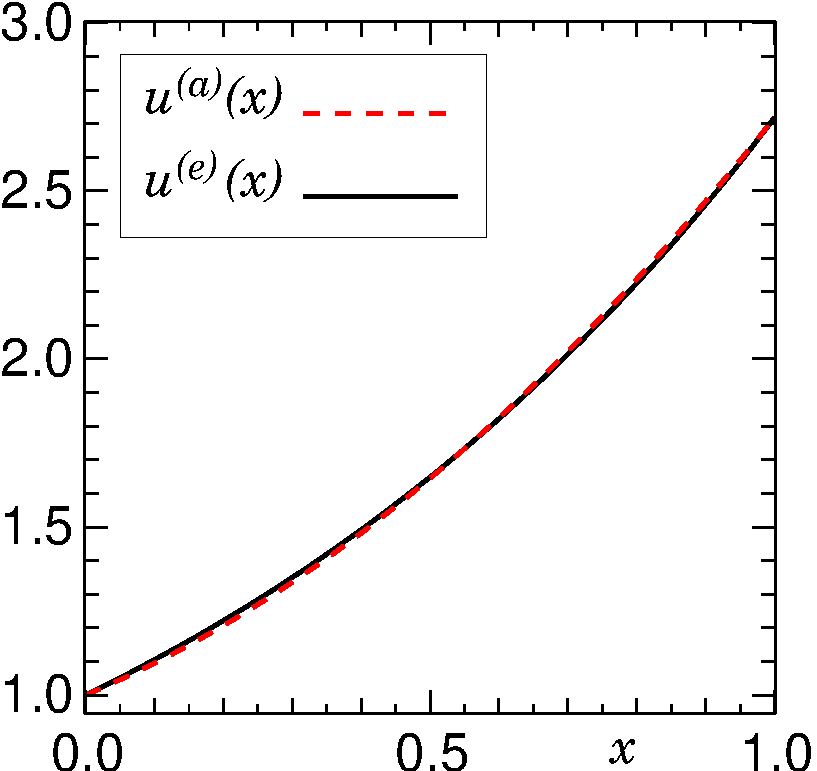
\includegraphics[width=80mm]{figures/ColloEner}}
  \caption{\label{fig:ColloEner} \it Graphs of the exact
    [Eq.~(\ref{cwk4.eq:3})] and approximate [Eq.~(\ref{eq:12})]
    solution of the boundary value problem~(\ref{cwk4.eq:4}).}
\end{figure}

The left boundary condition fixes $c_0$:
%
\begin{equation}
  u^{(a)}(0) = c_0 = 1 .
  \label{eq:9}
\end{equation}
%
The right boundary condition gives a relation between $c_1$ and $c_2$:
%
\begin{equation}
  u^{(a)}(1) = c_0 + c_1 + c_2 = e \implies c_1 = e - 1 - c_2 .
  \label{eq:8}
\end{equation}
%
Substituting~(\ref{eq:9}) and~(\ref{eq:8}) into~(\ref{cwk4.eq:4})
gives that $F(c_j)$ defined by~(\ref{eq:10}) is
%
\begin{equation}
  F(c_2) = \frac{47}{10} c_2^2 - \frac{13}{6}(1+e)c_2 + \frac{1+e+e^2}{3} .
  \label{eq:11}
\end{equation}
%
We solve for $c_2$ by requiring that $F(c_2)$ is as small as possible,
i.e.\ that the derivative of $F(c_2)$ with respect to $c_2$ is zero.
Differentiating~(\ref{eq:11}) we obtain
%
\begin{equation*}
 \dv{F}{c_2} = \frac{47}{5} c_2 - \frac{13}{6}(1+e) = 0 \implies
 c_2 = \frac{65}{282}(1+e) ,
\end{equation*}
%
so that from equation~(\ref{eq:8}) we have
%
\begin{equation*}
  c_1 = \frac{217 e - 347}{282}
\end{equation*}
%
and the approximate solution of the boundary value
problem~(\ref{cwk4.eq:4}) is
%
\begin{equation}
  u^{(a)}(x) = 1 + \frac{217 e - 347}{282} x + \frac{65}{282}(1+e) x^2 .
  \label{eq:12}
\end{equation}
%
The graphs of the approximate and exact solutions are shown in
Figure~\ref{fig:ColloEner}: the match is pretty impressive for a three
node approximation.

\subsection{The collocation method}

In the \textit{collocation} method we substitute the approximate
solution~(\ref{cwk4.eq:2}) in~(\ref{cwk4.eq:1}),
%
\begin{equation*}
  \mathcal{L} \sum_{j=1}^n c_j v_j(x) = w(x) \implies
  \sum_{j=1}^n c_j \mathcal{L} v_j(x) = w(x) ,
\end{equation*}
%
and we require that this equation should be satisfied at a set of $n$
\textit{collocation points} $\{x_j\}$, i.e.\ that the coefficients
$c_j$ are the solution of the system of linear equations
%
\begin{equation*}
  \sum_{j=1}^n c_j \mathcal{L} v_j(x_k) = w(x_k) , \qquad k=1,2,\ldots,n.
\end{equation*}
%
Note that the values of the basis functions $v_j(x)$ at the
collocation points $x_k$ should be such that the matrix of the
coefficients of this system is non-singular.

\begin{figure}
  \centerline{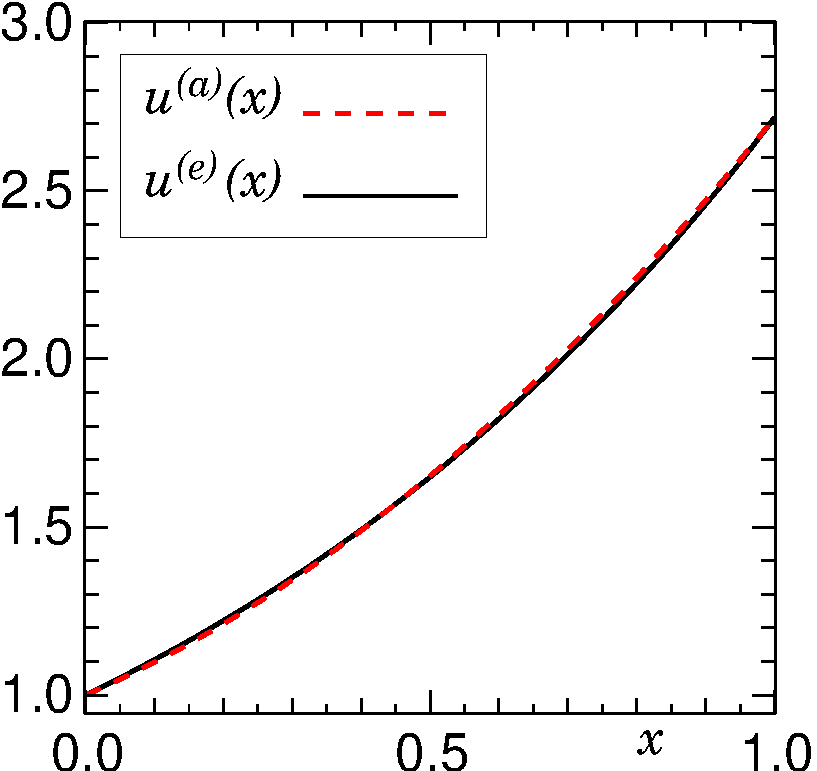
\includegraphics[width=80mm]{figures/Collocation}}
  \caption{\label{fig:Collocation} \it Graphs of the exact
    [Eq.~(\ref{cwk4.eq:3})] and approximate [Eq.~(\ref{eq:13})]
    solution of the boundary value problem~(\ref{cwk4.eq:4}).}
\end{figure}

Once again consider as an example the boundary value
problem~(\ref{cwk4.eq:4}) and write the approximate solution as in
equation~(\ref{cwk4.eq:5}).  We require that it should satisfy the
boundary conditions as in equations~(\ref{eq:9}) and~(\ref{eq:8}), so
that the approximate solution is now given by
%
\begin{equation*}
  u^{(a)}(x) = 1 + (e-1-c_2) x + c_2 x^2 .
\end{equation*}
%
Finally, we require that this function should satisfy the differential
equation~(\ref{cwk4.eq:4}) at $x=1/2$.  Taking into account that
%
\begin{equation*}
 \dv[2]{}{x} u^{(a)}(x) = 2 c_2
\end{equation*}
%
we have that this requirement is equivalent to
%
\begin{equation*}
  2 c_2 - \left [ 1 + (e-1-c_2) \frac{1}{2} +
    c_2 \left ( \frac{1}{2} \right )^2 \right ] = 0 \implies
  c_2 = \frac{2}{9}(1+e) \implies c_1 = \frac{7 e - 11}{9}
\end{equation*}
%
so that the approximate solution is given by
%
\begin{equation}
  u^{(a)}(x) = 1 + \frac{7 e - 11}{9} x + \frac{2}{9}(1+e) x^2 .
  \label{eq:13}
\end{equation}
%
The graphs of the approximate and exact solutions are shown in
Figure~\ref{fig:Collocation}: the match is pretty impressive for a
three node approximation and is comparable, but different, from that
in Figure~\ref{fig:ColloEner}.

\smallskip

\noindent \textbf{Remark} - In general it is not advisable to use as
basis functions the powers of $x$ or a uniformly spaced set of nodes.
Orthogonal polynomials (like the Legendre and the Chebyschev
polynomials) and non-uniform grids (e.g. Gauss-Lobatto grids) give
more accurate and numerically stable results.


\section*{Further reading}

Topics covered here are also covered in
\begin{itemize}
\item Chapter 11 of Linz \& Wang, \textit{Exploring Numerical Methods}
  (QA297 LIN),
\item Chapter 8 of Kincaid \& Cheney, \textit{Numerical Analysis}
  (QA297 KIN),
\item Chapter 13 (and to some extent 14) of S{\"u}li \& Mayers,
  \textit{An Introduction to Numerical Analysis} (not in library).
\end{itemize}


\chapter[Partial Differential Equations]{Finite difference methods for Partial Differential Equations}

\section[Revision]{Revision of Partial Differential Equations}

A {\em partial differential equation} is a relation between the
partial derivatives of an unknown function and the independent
variables.  The order of the highest derivative is called the {\em
  order} of the equation.

Just as in the case of an ordinary differential equation, we say that
a partial differential equation is {\em linear} if it is of the first
degree in the dependent variable (the unknown function) and its
partial derivatives.  If each term of such equation contains either
the dependent variable or one of its derivatives, the equation is
called {\em homogeneous}; otherwise it is said to be {\em non
  homogeneous}.

\smallskip

\noindent
{\bf Example} - The equations
%
\begin{eqnarray*}
  (a) & & \pdv{\phi}{t} - \pdv[2]{\phi}{x} = 0, \\
  (b) & & \phi(x,t) \pdv[2]{\phi}{t} + \pdv{\phi}{x} = f(x,t), \\
  (c) & & \pdv[4]{\phi}{x} + \pdv[4]{\phi}{y} = g(x,y) ,
\end{eqnarray*}
%
are, respectively, (a) Linear, homogeneous, second order, (b)
nonlinear, non-homogeneous, second order, (c) linear, non-homogeneous,
fourth order.

\smallskip

In this unit we consider only second order linear partial differential
equations with constant coefficients:
%
\begin{equation*}
  A \pdv[2]{u}{x} + 2 B \pdv{u}{x}{y} +
  C \pdv[2]{u}{y} + D \pdv{u}{x} + E \pdv{u}{y} = f(x,y) .
\end{equation*}
%
These equations are classified in three groups\footnote{Note that the
  coefficients $A$, $B$, etc. need not be constant}:

\medskip

\begin{center}
  \begin{tabular}{|l|l|l|l|} \hline
    \multicolumn{1}{|c|}{ Type} &
    \multicolumn{1}{c|}{Coefficients} &
    \multicolumn{1}{c|} {Typical form} &
    \multicolumn{1}{c|} {Name} \\ \hline \hline
    Hyperbolic & $B^2 - 4 A C > 0 $ &
    $u_{t t} - c^2 u_{x x} = 0 $ & Wave eq. \\ \hline
    Parabolic & $B^2 - 4 A C = 0 $ &
    $u_{t} - c^2 u_{x x} = 0 $ & Heat eq. \\ \hline
    Elliptic & $B^2 - 4 A C < 0 $ &
    $u_{x x} + u_{y y} = 0 $ & Laplace eq. \\ \hline
  \end{tabular}
\end{center}

\medskip

\noindent
The names arise by analogy with the curve
%
\begin{equation*}
  a x^2 + 2 b x y + c y^2 = f,
\end{equation*}
%
which represents an hyperbola, parabola and ellipse according as $b^2
- 4 a c$ is positive, zero or negative, respectively.

The classification of the equations is very important for the study of
their solutions.  A {\em solution} of a partial differential equation
in some region $R$ of the space of the independent variables is a
function that has all the partial derivatives that appear in the
equation and that satisfies the equation everywhere in $R$.  Like
ordinary differential equations, Partial differential equation have
many solutions.  For example, the functions
%
\begin{equation*}
  u(x,y) = x^2 - y^2, \quad u = e^x \cos(y), \quad u=\ln(x^2+y^2),
\end{equation*}
%
are all solutions of the equation
%
\begin{equation*}
  \pdv[2]{u}{x} + \pdv[2]{u}{y} = 0 .
\end{equation*}
%
Exactly like for ordinary differential equations we must specify
something more if we wish to obtain a unique solution: for example we
must specify the value of the function on the boundary of the region
$R$ ({\em boundary conditions}), and/or we must specify the value of
the function at the start ({\em initial conditions}).  What type of
boundary or initial condition to use depends on the type of Partial
differential equation.

\medskip

\centerline{\bf Hyperbolic}

\noindent \underline{Example}: $u_{t t} - c^2 u_{xx} = 0$.

\noindent \underline{Physical meaning}: Wave motion

\noindent \underline{Initial conditions}: The value of $u$ and its
time derivative at $t=0$: $u(x,0)=f(x)$ and $u_t(x,0)=g(x)$.

\noindent \underline{Boundary conditions}: Either $u$ or its normal
derivative at the boundary of the integration region: e.g. $u(0,t) =
\phi_1(t)$ and $u(L,t)= \phi_2(t)$.  The former type of boundary
condition is called a \textit{Dirichlet} boundary condition; the
latter is called a \textit{Neumann} boundary condition.  It is also
possible to mix the two types of boundary conditions (\textit{mixed
  boundary conditions}).

\bigskip

\centerline{\bf Parabolic}

\noindent \underline{Example}: $u_{t} - c^2 u_{xx} = 0$.

\noindent \underline{Physical meaning}: Heat diffusion

\noindent \underline{Initial conditions}: The value of $u$ at $t=0$:
$u(x,0)=f(x)$.

\noindent \underline{Boundary conditions}: Either $u$ or its normal
derivative at the boundary of the integration region: e.g. $u(0,t) =
\phi_1(t)$ and $u(L,t)= \phi_2(t)$.

\bigskip

\centerline{\bf Elliptic}

\noindent \underline{Example}: $u_{xx} + u_{y y} = 0$ (Laplace's
equation).

\noindent \underline{Physical meaning}: Stationary profile of a
membrane, stationary temperature profile of a metal plate,
electrostatic potential in the absence of charges.

\noindent \underline{Initial conditions}: They do not apply to these
equations.

\noindent \underline{Boundary conditions}: Either $u$ or its normal
derivative at the boundary of the integration region: e.g. if the
region is the rectangle $0 \le x \le a$, $0 \le y \le b$: $u(0,y) =
\phi_1(y)$, $u(a,y)= \phi_2(y)$, $u(x,0) = g_1(x)$ and, finally,
$u(x,b)=g_2(x)$.

\begin{figure}
  \centerline{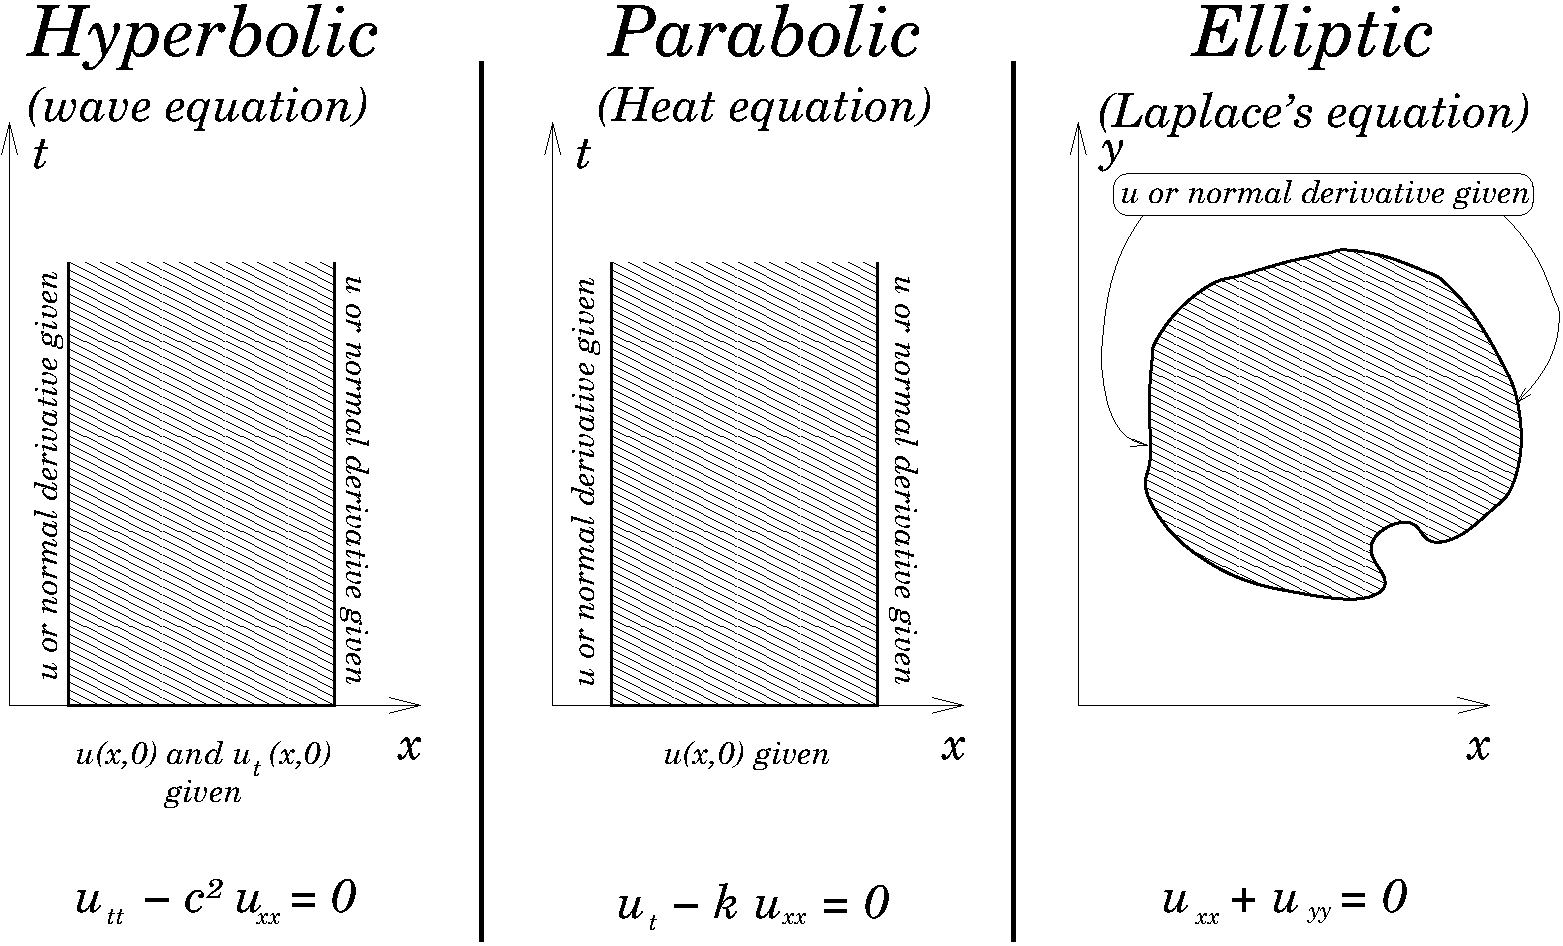
\includegraphics[width=120mm]{figures/pde_summary}}
  \caption{\label{fig:pde_summary} \it Types of partial differential
    equations and their boundary and initial conditions.}
\end{figure}

\section{Numerical methods for PDEs}

There are many classes of methods to solve numerically partial
differential equations.  Three main groups are:

\begin{enumerate}
  %
\item \textit{Finite difference methods}

  The differential operators are approximated using their finite
  difference representation on a given grid.  In this way the Partial
  Differential Equation is transformed to a (nonlinear) algebraic
  equation for the values of the solution on the grid points.  These
  are the only methods that we discuss at any length in this unit.
  %
\item \textit{Finite element methods}

  The domain of the solution is divided into cells.  The solution is
  represented as a simple function (e.g.\ a linear function) on each
  cell and the partial differential equation is transformed to an
  algebraic problem for the matching conditions of the simple
  solutions at the boundaries of the cells.
  %
\item \textit{Spectral methods}

  The solution is represented by a superposition of known functions
  (e.g. trigonometric functions or special polynomials).  The partial
  differential equation is transformed to a set of algebraic equations
  or ordinary differential equations for the amplitudes of the
  component functions.  A subclass of these methods are the
  \textit{collocation methods}: the solution is represented on a grid
  and the decomposition of the solution in known functions is used to
  estimate to a high degree of accuracy the partial derivatives of the
  solution on the grid points.  These methods are highly accurate and
  fast, but in general require the domain of the solution to be fairly
  simple, e.g.\ a rectangle.
  %
\end{enumerate}

\section[Elliptic Equations]{Elliptic Equations}

\subsection{Introduction}

A ``standard form'' of elliptic partial differential equation with
Dirichlet boundary conditions is
%
\begin{equation}
  \left\{
    \begin{aligned}
      u_{xx} + u_{y y} & = f(x,y), & & {\rm in}~~\Omega,\\
      u\big |_{\partial\Omega} & = \phi(x,y), & & {\rm on}~~\partial\Omega.
    \end{aligned}
  \right.\label{dp}
\end{equation}
%
This problem has a unique solution if the domain $\Omega$ has a smooth
boundary and $f$ and $\phi$ are continuous functions.

\subsection{A simple finite difference method}

We are going to solve equation~(\ref{dp}) numerically using the method
of finite differences.  At the heart of this method is the finite
difference approximation of the second derivative of a function
$y(x)$:
%
\begin{equation}
  y''(x) = \frac{1}{h^2}[y(x+h)+y(x-h)-2y(x)]-
  \frac{h^2}{12}y^{(4)}(\xi), \label{fd}
\end{equation}
%
where $h$ is a fixed step size.  We illustrate this method using a
simple case of equation~(\ref{dp}), namely the case of a Dirichlet
problem on a rectangle $0<x<a$, $0<y<b$.  First, a network of grid
points is established on the rectangle:
%
\begin{equation*}
  (x_i,y_j)=(i h_x,j h_y), \qquad 0\le i\le n+1, \quad 0\le j\le m+1,
\end{equation*}
%
where the step sizes in the $x$ and $y$ directions are given by
\begin{equation*}
  h_x=\frac{a}{n+1}, \qquad h_y=\frac{b}{m+1}.
\end{equation*}
%
Next, the differential equation in (\ref{dp}) at the mesh point
$(x_i,y_j)$ is replaced by its finite-difference analogue at that
point, which for $1 \le i \le n$ and $1 \le j \le m$ is:
%
\begin{align}
  \label{eq:ellfd}
  & & \frac{1}{h_x^2}[u_{i-1,j}+u_{i+1,j}-2u_{i,j}] +
  \frac{1}{h_y^2}[u_{i,j-1}+u_{i,j+1}-2u_{i,j}] & = f_{i j},
  \nonumber \\
  \implies & & u_{i-1,j}+u_{i+1,j}-2u_{i,j} + \alpha
  [u_{i,j-1}+u_{i,j+1}-2u_{i,j}] & = h^2f_{i,j},
\end{align}
%
where $u_{i,j} = u(x_i,x_j)$, $\alpha=(h_x/h_y)^2$ and $h=h_x$.  The
values of $u_{i,j}$ are known when $i=0$ or $n+1$ and when $j=0$ or
$m+1$, since these are the prescribed boundary values in the problem:
%
\begin{align*}
  u_{0,j} & = \phi(x_0,y_j)  = \phi(0,y_j) , &
  u_{i,0} & = \phi(x_i,y_0)  = \phi(x_i,0), \\
  u_{n+1,j} & = \phi(x_{n+1},y_j)  = \phi(a,y_j), &
  u_{i,m+1} & = \phi(x_i,y_{m+1})  = \phi(x_i,b).
\end{align*}
%
This means that equation~(\ref{dp}) has been transformed to a
non-homogeneous system of linear equations, given by~(\ref{eq:ellfd}),
with unknowns $u_{i,j}$ and $1\le i\le n$, $1\le j\le m$.

As an example, consider the simple case $n=2$ and $m=3$.  The
approximate solution of equation~(\ref{dp}) at the grid points are the
solution of the $6\times 6$ system
%
\begin{eqnarray*}
  & & [u_{01}-2u_{11}+u_{21}]+\alpha[u_{10}-2u_{11}+u_{12}]=h^2f_{11},\\
  & & [u_{02}-2u_{12}+u_{22}]+\alpha[u_{11}-2u_{12}+u_{13}]=h^2f_{12},\\
  & & [u_{03}-2u_{13}+u_{23}]+\alpha[u_{12}-2u_{13}+u_{14}]=h^2f_{13},\\
  & & [u_{11}-2u_{21}+u_{31}]+\alpha[u_{20}-2u_{21}+u_{22}]=h^2f_{21},\\
  & & [u_{12}-2u_{22}+u_{32}]+\alpha[u_{21}-2u_{22}+u_{23}]=h^2f_{22},\\
  & & [u_{13}-2u_{23}+u_{33}]+\alpha[u_{22}-2u_{23}+u_{24}]=h^2f_{23}.
\end{eqnarray*}
%
The unknown quantities in this problem can be ordered in many ways. We
select the one known as the natural ordering
%
\begin{equation*}
  u=[u_{11},u_{12},u_{13},u_{21},u_{22},u_{23}]^T.
\end{equation*}
%
The system has the form $A \bu = \bF$ with
%
\begin{equation}
  A = \left ( \begin{array}{cccccc}
      -2 (1+\alpha) & \alpha & 0 & 1 & 0 & 0 \\
      \alpha & -2(1+\alpha) & \alpha & 0 & 1 & 0 \\
      0 & \alpha & -2(1+\alpha) & 0 & 0 & 1 \\
      1 & 0 & 0 & -2(1+\alpha) & \alpha & 0 \\
      0 & 1 & 0 & \alpha & -2(1+\alpha) & \alpha \\
      0 & 0 & 1 & 0 & \alpha & -2(1+\alpha) \\
    \end{array} \right ) \label{eq:PDE:A}
\end{equation}
%
and
%
\begin{equation*}
  \bF =
  \begin{pmatrix}
    h^2f_{11}- u_{01}-\alpha u_{10} \\
    h^2f_{12}- u_{02} \\
    h^2f_{13}- u_{03}-\alpha u_{14} \\
    h^2f_{21}- u_{31}-\alpha u_{20} \\
    h^2f_{22}- u_{32} \\
    h^2f_{23}- u_{33}-\alpha u_{24}
  \end{pmatrix},
\end{equation*}
%
where in the expressions of the components of the vector $\bF$ only
the boundary values of $u_{i,j}$ are present.

In general, the $n\times m$ system is sparse because each equation
contains at most five unknowns.  Iterative procedures such as the
Gauss-Seidel iterative method can be quite effective in this
situation.  Moreover, in setting up such a procedure there is no need
to store the matrix $A$ of the coefficients defined in
equation~(\ref{eq:PDE:A}).  In fact, we can rewrite
equation~(\ref{eq:ellfd}) as
%
\begin{equation}
  u_{i,j} = \frac{1}{2(1+\alpha)} \left [ u_{i-1,j} +u_{i+1,j} +
    \alpha (u_{i,j-1}+u_{i,j+1}) - h^2 f_{i,j} \right ], \quad
  1 \le i \le n, \, 1 \le j \le m . \label{PDE:eq:Ell:Updateuij}
\end{equation}
%
This equation is a Gauss-Seidel formula to update $u_{i,j}$. When this
equation is used, the value obtained from the right-hand side replaces
the old value of $u_{i,j}$.  It can also be seen as an implementation
of Jacobi's method, if we assume that the variable on the left-hand
side are stored separately from those on the right hand side.  As
initial guess of the solution we can assume that $u_{i,j} \equiv 0$
(in general we should use a guess that satisfies the boundary
conditions).  Of course an initial guess close to the solution will
reduce the number of iterations needed for convergence.

\subsection{Error analysis}

How accurate is the solution obtained using~(\ref{eq:ellfd}) or,
equivalently~(\ref{PDE:eq:Ell:Updateuij})? To answer this question
we introduce the error
%
\begin{equation*}
  e_{i,j}=u_{i,j}-\hat u_{i,j},
\end{equation*}
%
where $\hat u_{i,j}=u(x_i,y_j)$ are the values of the exact solution
of equation~(\ref{dp}). Substituting
%
\begin{equation*}
  u_{i,j}=e_{i,j}+\hat u_{i,j}
\end{equation*}
%
into the difference equation~(\ref{eq:ellfd}), we obtain
%
\begin{eqnarray*}
 & & \frac{1}{h_x^2}[e_{i-1,j}+e_{i+1,j}-2e_{i,j}] +
      \frac{1}{h_y^2}[e_{i,j-1}+e_{i,j+1}-2e_{i,j}] = \\
 & & \hspace{10mm} f_{i,j} -
     \frac{1}{h_x^2}[\hat u_{i-1,j}+\hat u_{i+1,j}-2\hat u_{i,j}] -
     \frac{1}{h_y^2}[\hat u_{i,j-1}+\hat u_{i,j+1}-2\hat u_{i,j}].
\end{eqnarray*}
%
Using the finite-difference approximation formula~(\ref{fd}) to
eliminate the finite differences we obtain
%
\begin{align*}
  \frac{1}{h_x^2}[e_{i-1,j}+e_{i+1,j}-2e_{i,j}] +
     \frac{1}{h_y^2}[e_{i,j-1}+e_{i,j+1}-2e_{i,j}] & =
     f_{i,j} - \\
     & \quad [u_{xx}(x_i,y_j) + \frac{h_x^2}{12}u_{xxxx}(\xi_i,y_i)] -
     \\
     & \quad [u_{y y}(x_i,y_j)+\frac{h_2^2}{12}u_{yyyy}(x_i,\zeta_j)] \\
     & = - \frac{h_x^2}{12}u_{xxxx}(\xi_i,y_i) -
     \frac{h_y^2}{12}u_{yyyy}(x_i,\zeta_j)
\end{align*}
%
where we have used
%
\begin{equation*}
  u_{xx}(x_i,y_j)+u_{y y}(x_i,y_j)=f_{i.j}.
\end{equation*}
%
Hence, the error satisfies the difference equation
%
\begin{equation*}
  e_{i-1,j}+e_{i+1,j}-2e_{i,j}+\alpha[e_{i,j-1}+e_{i,j+1}-2e_{i,j}]=
  -\frac{h_x^4}{12}u_{xxxx}(\xi_i,y_i)-
  \frac{h_x^2 h_y^2}{12}u_{yyyy}(x_i,\zeta_j),
\end{equation*}
%
and zero boundary conditions. Analysing this equality, it is possible
to prove that
%
\begin{equation*}
  ||e_{i,j}|| \simeq \order{h_x h_y}.
\end{equation*}
%
This means that in the limit $n\to +\infty$ and $m\to +\infty$ the
norm of the error tends to zero.

\section{Parabolic Equations}

\subsection{Introduction}

Throughout this section we assume that the parabolic equation to be
solved is
%
\begin{equation}
  \pdv{u}{t} = \pdv[2]{u}{x} , \qquad 0 \le x \le 1, \, 0 \le t
  \label{PDE:eq:Para:template}
\end{equation}
%
with boundary conditions
%
\begin{equation*}
  u(0,t) = 0, \qquad u(1,t) = 0,
\end{equation*}
%
and initial condition $u(x,0) = g(x)$.  There are many finite
difference methods to solve equation~(\ref{PDE:eq:Para:template}).
Here we consider only a few that are typical examples of their
respective classes.  Moreover, it should be noted that
equation~(\ref{PDE:eq:Para:template}) is linear.  The methods that we
discuss become much harder to implement in the case of nonlinear
equations.

\subsection[Forward-Time, Centred-Space (FTCS)]{An explicit method - Forward-Time, Centred-Space (FTCS)}

\subsubsection{The method}

We fix a time discretisation step $\delta$ and a space discretisation
step $h$ so that the solution of equation~(\ref{PDE:eq:Para:template})
is represented on the grid
%
\begin{equation*}
  (x_i,t^n) = (i h, n \delta), \qquad 0 \le i \le N + 1, \, n \ge 0
\end{equation*}
%
where the number of grid points between $x=0$ and $x=1$ is $N+2$.  We
use the notation $u_i^n$ to indicate $u(x_i,t^n)$.  We discretise the
time derivative in equation~(\ref{PDE:eq:Para:template}) using a
forward difference approximation
%
\begin{equation}
  \pdv{u}{t} = \frac{u_i^{n+1}-u_i^{n}}{\delta} + \order{\delta}
  \label{PDE:eq:ut}
\end{equation}
%
and the spatial derivative using
%
\begin{equation}
  \pdv[2]{u}{x} = \frac{u_{i+1}^{n}+u_{i-1}^{n}-2u_{i}^{n}}{h^2} + \order{h^2}
  \label{PDE:eq:uxx}
\end{equation}
%
so that equation~(\ref{PDE:eq:Para:template}) is represented by the
set of (linear) algebraic equations
%
\begin{equation*}
  u_{i}^{n+1} = u_{i}^{n} +
  \frac{\delta}{h^2} (u_{i+1}^{n}+u_{i-1}^{n}-2u_{i}^{n})
\end{equation*}
%
or, equivalently,
%
\begin{equation}
  u_{i}^{n+1} = (1-2s) u_{i}^{n} + s (u_{i+1}^{n}+u_{i-1}^{n})
  \label{PDE:eq:Para:expl}
\end{equation}
%
where $s = \delta/h^2$.  Equation~(\ref{PDE:eq:Para:expl}) is a finite
difference representation of Equation~(\ref{PDE:eq:Para:template}):
since this equation gives the new values of $u_{i}^{n+1}$ explicitly
in terms of previous values of $u_{i+1}^{n}$, $u_{i}^{n}$ and
$u_{i-1}^{n}$ the method based on this equation is called an
\textit{explicit method}.  As it involves a forward difference
approximation of the time derivative and a centred approximation of
the spatial derivative it is called a \textit{forward-time
  centred-space} (FTCS) method.

Equation~(\ref{PDE:eq:Para:expl}) must be complemented by the
discretized version of the initial and boundary conditions, namely
%
\begin{equation*}
  u_{0}^{n} = u_{N+1}^{n} = 0 \qand u_{i}^{0} = g(x_i) .
\end{equation*}

\subsubsection{Consistency, Stability and Convergence}

We have claimed that equation~(\ref{PDE:eq:Para:expl}) is a finite
difference representation of equation~(\ref{PDE:eq:Para:template}) and
that, therefore, can be used to find an accurate numerical solution to
this equation.  Given any algorithm to solve numerically a partial
differential equation we must clearly determine if it is ``good'', in
the sense that it can be used to obtain efficiently an accurate
solution of the problem we aim to solve.  In order to do this we must
define clearly what we mean by a ``good method''.

\begin{enumerate}
  %
\item A finite difference equation is \textbf{consistent} with a
  partial differential equation if the difference between the Finite
  Difference Equation (FDE) and the PDE (i.e. the truncation error)
  vanishes as the sizes of the grid spacings go to zero independently.

  When the truncation error of the finite difference approximations of
  the individual exact partial derivatives are known, proof of
  consistency is straightforward. When the truncation errors of the
  individual finite difference approximations are not known, the
  complete finite difference equation must be analysed for
  consistency.  That is accomplished by expressing each term in the
  finite difference equation by a Taylor series about a particular
  grid point.  The resulting equation, which is called the modified
  differential equation (MDE), can be simplified to yield the exact
  form of the truncation error of the complete finite difference
  equation.  We will not develop this concept further in this unit.
  %
\item The \textbf{order} of a finite difference approximation of a
  partial differential equation is the rate at which the global error
  of the finite difference solution approaches zero as the size of the
  grid spacings approach zero.

  The global error of a finite difference equation is the order of the
  truncation error terms in the finite difference approximations of
  the individual exact partial derivatives in the Partial Differential
  Equation.
  %
\item When applied to a partial differential equation that has a
  bounded solution, a finite difference equation is \textbf{stable} if
  it produces a bounded solution and is unstable otherwise.

  If the solution of the FDE is bounded for all values of the grid
  spacings, then the FDE is \textit{unconditionally stable}.  If the
  solution of the FDE is bounded only for certain values of the grid
  spacings, then the FDE is \textit{conditionally stable}.  If the
  solution of the FDE is unbounded for all values of the grid
  spacings, then the FDE is \textit{unconditionally unstable}.  The
  most used method to prove the stability of a (linear) finite
  difference scheme is the Von Neumann method (see below).
  %
\item A finite difference method is \textbf{convergent} if the
  solution of the finite difference equation approaches the exact
  solution of the partial differential equation as the sizes of the
  grid spacings go to zero.

  Convergence is the most desirable property of an integration scheme.
  However it is quite hard to prove directly that a method is
  convergent.
%
\end{enumerate}

Consistency, stability and convergence are not independent concepts.
They are related by the following theorem due to Lax (1954):

\begin{quote}
  %
  Given a properly posed linear initial-value problem and a finite
  difference approximation to it that is consistent, stability is the
  necessary and sufficient condition for convergence.
  %
\end{quote}

Thus, the question of convergence of a finite difference method is
answered by a study of the consistency and stability of the finite
difference equation.  If the finite difference equation is consistent
and stable, then the finite difference method is convergent.

The Lax equivalence theorem applies to well-posed linear initial-value
problems.  May problems in engineering and science are not linear and
nearly all problems involve boundary conditions in addition to initial
conditions.  There is no equivalence theorem for such problems.
Nonlinear PDEs must be linearised locally and the FDE that
approximates the linearised PDE is analysed for stability.  Experience
has shown that the stability criteria obtained of the linearised FDE
also apply to the nonlinear FDE and that FDEs that are consistent and
whose linearised equivalent is stable generally converge even for
nonlinear initial-boundary-value problems.

\subsubsection{Consistency, stability and convergence of a FTCS
method}

Equation~(\ref{PDE:eq:Para:expl}) is first order in time and second
order in space: in fact the error involved in the discretisation of
the time derivative, equation~(\ref{PDE:eq:ut}), is $\order{\delta}$, while
the error in the discretisation of the space derivative,
equation~(\ref{PDE:eq:uxx}), is $\order{h^2}$.

Equation~(\ref{PDE:eq:Para:expl}) is clearly consistent.  As $\delta
\to 0$ and $h \to 0$ the finite difference approximations of the time
and space derivatives, equations~(\ref{PDE:eq:ut},~\ref{PDE:eq:uxx}),
converge to the respective derivatives.

To verify whether the method given by
equation~(\ref{PDE:eq:Para:expl}) is stable, we start by observing
that the solution of equation~(\ref{PDE:eq:Para:template}) with
boundary conditions $u(0,t)=u(1,t)=0$ tends to zero in the long time
limit whatever the initial condition $g(x)$.  Therefore, also the
solution of the finite difference approximation,
equation~(\ref{PDE:eq:Para:expl}), must tend to zero as the time
discretisation index $n$ tends to infinity.  To verify whether this is
the case we use the \textit{Von Neumann method}.  The solution of
equation~(\ref{PDE:eq:Para:expl}) is of the form
%
\begin{equation}
  u_{\ell}^{k} = e^{\tj \alpha \ell h} q^k
  \label{PDE:eq:uellk}
\end{equation}
%
where $\tj = \sqrt{-1}$ while $\alpha$ and $q$ are real parameters
that have to be determined by requiring that~(\ref{PDE:eq:uellk})
satisfies~(\ref{PDE:eq:Para:expl}).  Substituting~(\ref{PDE:eq:uellk})
into~(\ref{PDE:eq:Para:expl}) we obtain that $q$ is given by
%
\begin{equation*}
  q = s \left ( e^{\tj \alpha h} + e^{-\tj \alpha h} \right ) + (1 - 2s) =
  1 - 4 s \sin^2 \left ( \frac{\alpha h}{2} \right ) .
\end{equation*}
%
In order for $|u_{\ell}^{k}|$ to decrease to zero as $k$ tends to
infinity we must have
%
\begin{equation}
  |q| < 1 \implies s < \frac{1}{2} \implies
  \frac{\delta}{h^2} < \frac{1}{2} .
  \label{PDE:eq:FTCSConstr}
\end{equation}
%
In other words, the FTCS method~(\ref{PDE:eq:Para:expl}) is only
conditionally stable and the time and space discretisation steps,
$\delta$ and $h$ respectively, must satisfy the
constraint~(\ref{PDE:eq:FTCSConstr}).  Using the Lax theorem we can
therefore conclude that, under these conditions, the FTCS method is
also convergent.  However, equation~(\ref{PDE:eq:FTCSConstr}) is a
rather stringent constraint as the time step must be reduce by a
factor of four if the space step is halved.  Therefore, methods
like~(\ref{PDE:eq:Para:expl}) tend to be rather slow.

\subsection[Backward-Time, Centred-Space (BTCS)]{An Implicit method - Backward-Time, Centred-Space (BTCS)}

\subsubsection{The method}

In the explicit finite difference approximation of the diffusion
equation the right hand side of equation~(\ref{PDE:eq:Para:template})
is computed at the current time step and used to compute the value of
the solution at the next time step.  In the implicit finite difference
approximation the right hand side is ``computed'' at the next time
step, so that the finite difference scheme is an implicit equation for
the new value of the solution.  In the case of
equation~(\ref{PDE:eq:Para:template}) this is accomplished by using a
backward difference approximation of the time derivative at
$t^{n+1}=t+\delta$ so that equation~(\ref{PDE:eq:Para:template}) is
discretised as
%
\begin{align}
 && \frac{u_{i}^{n+1} - u_{i}^{n}}{\delta} & =
       \frac{u_{i+1}^{n+1}+u_{i-1}^{n+1}-2u_{i}^{n+1}}{h^2} \nonumber \\
 \implies && (1+2s) u_{i}^{n+1} & = u_{i}^{n} + s
 (u_{i+1}^{n+1}+u_{i-1}^{n+1})
 \label{PDE:eq:Para:BTCS}
\end{align}
%
where $s = \delta/h^2$ and the unknowns are all the $u_{i}^{n+1}$.
Equation~(\ref{PDE:eq:Para:BTCS}) constitutes of a tri-diagonal linear
system for the unknowns $u_{i}^{n}$ with row
%
\begin{equation*}
  -s u_{i-1}^{n+1} + (1+2s) u_{i}^{n+1} - s u_{i+1}^{n+1} = u_{i}^{n},
  \qquad 1 \le i \le N .
\end{equation*}
%
This system can be solved by Gaussian elimination.  Note, however,
that if the partial differential equation is nonlinear then
equation~(\ref{PDE:eq:Para:BTCS}) becomes a nonlinear algebraic
equation for the unknowns $u_{i}^{n+1}$ and is, as a consequence, very
hard to solve.

\subsubsection{Consistency, stability and convergence}

Like the FTCS method, the BTCS is first order in time and second order
in space.  Moreover, it is clearly consistent.

The stability analysis is very similar to that of the explicit method.
We look for a solution of equation~(\ref{PDE:eq:Para:BTCS}) of the
form (\ref{PDE:eq:uellk}) and substitute it in
equation~(\ref{PDE:eq:Para:BTCS}).  We obtain that $q$ must satisfy
%
\begin{equation*}
  q = 1 + 2 s \left ( e^{\tj \alpha h} + e^{-\tj \alpha h} - 2 \right ) q \implies
  q = \frac{1}{1 + 4 s \sin^2 \left ( \frac{\alpha h}{2} \right )} \, .
\end{equation*}
%
In other words $|q| < 1$ for all values of $s$ and the backward-time,
centred space method is unconditionally stable and, hence,
unconditionally convergent.

\section{Hyperbolic Equations}

\subsection{Introduction}

The theory of hyperbolic equations and their solutions is quite
involved and is not studied in this unit.  However, it is essential to
know it and understand it if any serious work with hyperbolic partial
differential equations is to be attempted.  Here we consider a very
simple case and use it to discuss a few methods to integrate
hyperbolic partial differential equations.  The methods discussed
apply also to more complex cases, but care should be taken to ensure
that the solutions obtained are acceptable.

As an example of a hyperbolic equation we consider the advection
equation
%
\begin{equation}
  \pdv{u}{t} + v \pdv{u}{x} = 0 , \qquad a \le x, \quad v > 0 .
  \label{PDE:eq:advect}
\end{equation}
%
This equation represents a function propagating in the positive
$x$-direction with speed $v$.  In order for the equation to have a
unique solution we must specify an initial condition, $u(x,0) = F(x)$
and a boundary condition at $x=a$, $u(a,t) = G(t)$.  Note that the
domain is unbounded in the positive $x$-direction: numerically this
implies that the numerical solution of equation~(\ref{PDE:eq:advect})
is acceptable only if the effects of the right boundary are
negligible, i.e.\ only for the time taken for the signal to propagate
across the integration region and reach the right boundary.

\subsection{The forward-time centred-space method}

The most straightforward finite difference method for solving
hyperbolic partial differential equations would appear to be the
forward-time centred-space (FTCS) method.  Applied to the diffusion
equation this method is conditionally stable; however, when applied to
the convection equation this method is unconditionally unstable.  The
algorithm consists in replacing the time derivative in
equation~(\ref{PDE:eq:advect}) with its forward difference
approximation and the space derivative with the centred-difference
approximation.  We obtain:
%
\begin{equation*}
  \frac{u_{i}^{n+1}-u_{i}^{n}}{\delta} +
  v \frac{u_{i+1}^{n}-u_{i-1}^{n}}{2 h} = 0
\end{equation*}
%
where $\delta$ is the time step, $h$ is the space step, the spatial
grid is $x_i = i h$, with $i=0,1,\ldots,N+1$, the time grid is $t^n =
n \delta$ and $u_{i}^{n} = u(x_i,t^n)$.  Solving for $u_{i}^{n}$ we
obtain
%
\begin{equation}
  u_{i}^{n+1} = u_{i}^{n} - \frac{c}{2} (u_{i+1}^{n}-u_{i-1}^{n}) \, ,
  \label{PDE:eq:hypFTCS}
\end{equation}
%
where $c = u \delta/h$ is the \textit{convection number}.  The
stability analysis of this equation shows that the solution
of~(\ref{PDE:eq:hypFTCS}) is $u_{\ell}^{k} = \exp(\tj \alpha \ell h)
q^k$, with
%
\begin{equation*}
  q = 1 - \tj c \sin(\alpha h) ,
\end{equation*}
%
where $\tj = \sqrt{-1}$.  From this we obtain that
%
\begin{equation*}
  |q| = \sqrt{1 + c^2 \sin^2(\alpha h)} > 1 \, \, \forall c \in \bR .
\end{equation*}
%
Hence the FTCS method is unconditionally unstable.

\subsection{The Lax method}

Lax (1954) proposed a modification to the FTCS method for the
convection equation that yields a conditionally stable method.  In
that modification, the value $u_{i}^{n}$ in the finite difference
approximation of the time derivative is replaced by the average of its
values at the neighbouring points:
%
\begin{equation}
  u_{i}^{n+1} = \frac{1}{2} (u_{i+1}^{n} + u_{i-1}^{n}) -
  \frac{c}{2} (u_{i+1}^{n}-u_{i-1}^{n}) \, ,
  \label{PDE:eq:hypLax}
\end{equation}
%
This method is not consistent in general.  It can be shown that the
partial differential equation that is represented by
equation~(\ref{PDE:eq:hypLax}) is
%
\begin{equation}
  \pdv{u}{t} + v \pdv{u}{x} = \frac{1}{2}
  \left ( \frac{h^2}{\delta} - v^2 \delta \right )
  \pdv[2]{u}{x} +
  \frac{1}{3} \left ( v h^2 - v^3 \delta^2 \right ) \pdv[3]{u}{x} +
  \ldots \, ,
  \label{PDE:eq:LaxEquiv}
\end{equation}
%
where $h$ and $\delta$ are the space and time discretisation steps.
From this equation we can see that as $h$ and $\delta$ tend to zero
the first term on the right hand side does not vanish: on the
contrary, it is undetermined.  However, if the two discretisation
steps tend to zero so that their ratio is constant, for example at the
value $\beta = h / \delta$, then equation~(\ref{PDE:eq:hypLax})
approaches the equation
%
\begin{equation}
  \pdv{u}{t} + v \pdv{u}{x} = \frac{1}{2}
  \left ( \beta h - v^2 \delta \right )
  \pdv[2]{u}{x}
  \label{eq:PDE:LaxMDE}
\end{equation}
%
as $h$ and $\delta$ tend to zero.  The equation~(\ref{eq:PDE:LaxMDE})
is a parabolic convection-diffusion equation.  Substituting the
convection number $c=v \delta/h$ into equation~(\ref{eq:PDE:LaxMDE})
we obtain
%
\begin{equation}
  \pdv{u}{t} + v \pdv{u}{x} = \frac{1}{2} v h
  \left ( \frac{1}{c} - c \right ) \pdv[2]{u}{x}
  \label{eq:PDE:LaxMDE1}
\end{equation}
%
In other words if $c \neq 1$ the Lax approximation introduces some
numerical diffusion in the model that is to be integrated.  This
effect is common to most finite difference schemes: it is normally not
important if the original equation includes a diffusive term.  It may,
however, give completely false results if no diffusion terms are
present in the original equation.  In the case of the advection
equation the effect of the numerical diffusion is to smooth the
signals as they propagate and decrease their amplitude.


Another effect of the numerical diffusion of the Lax algorithm is to
make it conditionally stable.  The Von Neumann stability analysis
shows that the method is stable if
%
\begin{equation}
  c = \frac{v \delta}{h} \le 1 .
  \label{eq:PDE:hyp:CFL}
\end{equation}
%
Comparing this result with equation~(\ref{eq:PDE:LaxMDE1}) we see that
the scheme is stable if numerical diffusion is present.
Equation~(\ref{eq:PDE:hyp:CFL}) is called the Courant-Friedrichs-Lewy
stability criterion.  It states that the numerical speed of
propagation $v_{num} = h/ \delta$ must be greater than or equal to the
physical speed of propagation $v$.

\subsubsection{Derivation of Equation~(\ref{PDE:eq:LaxEquiv})}

To obtain equation~(\ref{PDE:eq:LaxEquiv}) we Taylor expand
$u_{i}^{n+1}$ and $u_{i\pm 1}^{n}$ around $u_{i}^{n}$ (indicated with
$u$ in what follows):
%
\begin{eqnarray*}
 & & u_{i}^{n+1} = u + \delta \partial_t u +
                 \frac{\delta^2}{2}\partial_{t t} u +
                 \frac{\delta^3}{3!} \partial_{t t t} u + \order{\delta^4}, \\
 & & u_{i\pm 1}^{n} = u + h \partial_x u \pm
                 \frac{h^2}{2}\partial_{x x} u \pm
                 \frac{h^3}{3!} \partial_{x x x} u + \order{h^4} .
\end{eqnarray*}
%
Substituting into equation~(\ref{PDE:eq:hypLax}) and dividing through
by $\delta$ we obtain
%
\begin{equation}
  \partial_t u + v \partial_x u =
  -\frac{\delta}{2} \partial_{t t} u
  -\frac{\delta^2}{6} \partial_{t t t} u
  + \frac{h^2}{2 \delta} \partial_{x x} u
  - \frac{v h^2}{6} \partial_{x x x}u + \order{\delta^3} + \order{h^3}
  \label{eq:PDE:14}
\end{equation}
%
We now wish to replace the derivatives with respect to time with
derivatives respect to space using this relation.  At first order in
$\delta$ we have that [we indicate with $\order{\delta^n}$ terms that are
of the order of $n$ in either $\delta$ or $h$]:
%
\begin{equation}
  \partial_t u = - v \partial_x u + \order{\delta}  \label{PDE:eq:16}
\end{equation}
%
so that
%
\begin{equation}
  \partial_{t t} u = - v \partial_x \partial_t u + \order{\delta} =
  v^2 \partial_{x x} u + \order{\delta}
  \label{PDE:eq:15}
\end{equation}
%
This is not accurate enough to be replaced into
equation~(\ref{eq:PDE:14}): we need to obtain an expression correct up
to second order in the space and time steps.  Starting once again from
equation~(\ref{eq:PDE:14}) we have
%
\begin{equation*}
  \partial_t u = -v \partial_x u
  - \frac{\delta}{2} \partial_{t t} u + \order{\delta^2} .
\end{equation*}
%
Differentiating with respect to time on both sides and making use
of~(\ref{PDE:eq:16}) and~(\ref{PDE:eq:15}) we obtain:
%
\begin{eqnarray*}
 \partial_{t t} u & = & -v \partial_x \partial_t u
   - \frac{\delta}{2} \partial_t \partial_{t t} u + \order{\delta^2} \\
  & = & -v \partial_x \left ( -v \partial_x u
   - \frac{\delta}{2} \partial_{t t} u \right )
   - \frac{\delta}{2} \partial_t v^2 \partial_{x x} u + \order{\delta^2} \\
  & = & v^2 \partial_{x x} u + v \partial_x
        \left ( \frac{\delta}{2} v^2 \partial_{x x} u \right ) +
      v^3 \frac{\delta}{2} \partial_{x x x} u + \order{\delta^2} \\
  & = & v^2 \partial_{x x} u + \delta v^3 \partial_{x x x} u +
      \order{\delta^2}.
\end{eqnarray*}
%
Differentiating equation~(\ref{PDE:eq:15}) with respect to time we
obtain
%
\begin{equation*}
  \partial_{t t t} u = -v^3 \partial_{x x x} u + \order{\delta} ,
\end{equation*}
%
and substituing both these expression into equation~(\ref{eq:PDE:14})
we (finally) obtain equation~(\ref{PDE:eq:LaxEquiv}).

\subsection{Upwind methods}

A salient feature of hyperbolic equations is that they describe the
propagation of information.  In the case of the advection
equation~(\ref{PDE:eq:advect}) the information propagates from
negative to positive $x$ with speed $v$.  This type of information
propagation is referred to as \textit{upwind} propagation, since the
information comes from the direction from which the convection
velocity comes, that is, the upwind direction.  Finite difference
methods that account for the upwind influence are called
\textit{upwind} methods.

The simplest procedure for developing an upwind finite difference
equation is to replace the time derivative by the first-order
forward-difference approximation and the space derivative by the
first-order one-sided-difference approximation in the upwind
direction.  For $v > 0$ the finite difference upwind approximation of
equation~(\ref{PDE:eq:advect}) is
%
\begin{equation}
  \frac{u_{i}^{n+1}-u_{i}^{n}}{\delta} + v
  \frac{u_{i}^{n} - u_{i-1}^{n}}{h} = 0 \implies
  u_{i}^{n+1} = u_{i}^{n} - c ( u_{i}^{n} - u_{i-1}^{n} ) ,
  \label{eq:PDE:Upw}
\end{equation}
%
where $c=v \delta/h$ is the convection number.  The upwind method is
consistent, first order in time and space and stable if $c \le 1$,
i.e. if the convection number satisfies the Courant-Friedrichs-Lewy
condition.  As in the case of the Lax scheme numerical diffusion (and
dispersion) is present unless $c=1$.

\section*{Further reading}

Topics covered here are also covered in
\begin{itemize}
\item Chapters 12 and 13 of Linz \& Wang, \textit{Exploring Numerical
    Methods} (QA297 LIN),
\item Chapter 9 of Kincaid \& Cheney, \textit{Numerical Analysis}
  (QA297 KIN),
\item Parts II and III (especially chapters 13 and 14) of Iserles,
  \textit{A First Course in the Numerical Analysis of Differential
    Equations} (QA297 ISE).
\end{itemize}



\chapter[Eigenvalues]{Eigenvalues}

\section{Introduction}

The eigenvalues and eigenvectors of a matrix are of fundamental
importance in many matrix problems: for example, in matrix
descriptions of physical models they often represent fundamental
physical quantities, like the energy levels of an atom or the
frequency of vibrations of a string.  In numerical analysis problems,
the eigenvalues determine the convergence conditions of many
iterations schemes, like Jacobi and Gauss-Seidel.

It is, therefore, important to be able to compute quickly and
accurately the eigenvalues and, eventually, the eigenvectors of a
square matrix.  This is an apparently simple problem that could be
tackled using standard nonlinear equations techniques.  In fact, the
eigenvalues $\lambda$ of a $n \times n$ square matrix $A$ are the $n$
roots of the characteristic polynomial of $A$,
%
\begin{equation*}
 \text{det}(A - \lambda \text{Id}) = 0 .
\end{equation*}
%
We could envisage using a root finding algorithm to detect all the
roots of the polynomial and, hence, all the eigenvalues of the matrix
$A$.  This is the procedure that is used in analytical calculations
when finding the eigenvalues of small ($2 \times 2$ or $3 \times 3$)
matrices.  However, roots of high order polynomials may be very
sensitive to the values of the coefficients: therefore, all the
unavoidable numerical errors involved in the lengthy calculation of
the coefficients of the characteristic polynomial of $A$ may well be
amplified at the stage of computing the roots and produce estimates
that bear very little relation to the eigenvalues of $A$.

\begin{Example}
  Polynomials may be badly conditioned, in the sense that a small
  change in the values of just one coefficient changes considerably
  the values of the roots.
\end{Example}

Consider the polynomial
%
\begin{align*}
 p(z) &= (z-1)\,(z-2)\,(z-3)\,(z-4)\,(z-5) \\
      &= -120 + 274 z - 225 z^2 + 85 z^3 - 15 z^4 + z^5 .
\end{align*}
%
The roots of this fifth order polynomial are quite obviously
$\{1,2,3,4,5\}$.  The roots of
%
\begin{equation*}
  p(z) = -120 + 274 z - 225 z^2 + 85 z^3 - 15 z^4 + 1.01 z^5
\end{equation*}
%
are $\{ 0.999, 2.067, 2.624, 4.580 \pm 0.966 \, i \, \}$ . \hfill
\rule{3mm}{3mm}

\smallskip

It is therefore necessary to develop techniques to identify the
eigenvalues of a matrix $A$ that do not rely on finding the roots of
the characteristic polynomial.

If we are interested in just a few eigenvalues then we can use one of
the many variations of the \textit{power method}.  Obtaining the full
spectrum is a much harder problem; an efficient algorithm to do so,
the $QR$-algorithm, was developed by J.G.F. Francis in 1961.  We
describe the power method first and give a relatively simple account
of the $QR$-algorithm after.  The chapter is based in its entirety on
the book by Kincaid and Cheney (chapter 5).%~\cite[Ch.~5]{kincaid96a}.

\section{The power method}

\subsection{The method}

The power method is an iterative procedure designed to compute the
dominant eigenvalue of a matrix and its corresponding eigenvector.
The method is based on two assumptions:

\begin{enumerate}
  %
\item There is a single eigenvalue of maximum modulus.
  %
\item There is a linearly independent set of $n$ eigenvectors, where
  $n$ is the size of the matrix.
  %
\end{enumerate}

According to the first assumption the eigenvalues of $A$ can be
labelled so that
%
\begin{equation*}
 |\lambda_1| > | \lambda_2 | \ge | \lambda_3 | \ge \ldots |\lambda_n|
\end{equation*}
%
According to the second assumption there is a basis of eigenvectors
$\{\bu_1, \bu_2, \ldots, \bu_n\}$ in $\bCn$ such that:
%
\begin{equation*}
 A \bu_j = \lambda_j \bu_j , \qquad 1 \le j \le n .
\end{equation*}

To start the iteration we need to define an initial vector $\bx^{(0)}$
and we have to require that its component along the eigenvector
$\bu_1$ is not zero:
%
\begin{equation*}
 \bx^{(0)} = \sum_{j=1}^n a_j \bu_j , \qquad a_1 \neq 0 .
\end{equation*}
%
Consider now the vector
%
\begin{equation*}
 \bx^{(k)} = A \bx^{(k-1)} = \ldots = A^k \bx^{(0)}.
\end{equation*}
%
Its decomposition on the basis of the eigenvectors is
%
\begin{equation*}
 \bx^{(k)} = \sum_{j=1}^n \lambda_j^k \bu_j =
             \lambda_1^k \left [ a_1 \bu_1 +
             \left ( \frac{\lambda_2}{\lambda_1} \right )^k a_2 \bu_2 +
             \left ( \frac{\lambda_3}{\lambda_1} \right )^k a_3 \bu_3 +
             \ldots
             \left ( \frac{\lambda_n}{\lambda_1} \right )^k a_n \bu_n
              \right ] .
\end{equation*}
%
We note that all the terms $\lambda_j/\lambda_1$, $j=2,3,\ldots,n$,
have modulus strictly smaller than one.  We can write this expression
as
%
\begin{equation}
  \bx^{(k)} = \lambda_1^k ( a_1 \bu_1 + \boldsymbol{\varepsilon}^{(k)} )
  \label{eq:Ev3}
\end{equation}
%
where
%
\begin{equation}
  \boldsymbol{\varepsilon}^{(k)} \equiv  \sum_{j=2}^n
  \left ( \frac{\lambda_j}{\lambda_1} \right )^k a_j \bu_j
  \label{eq:Ev5}
\end{equation}
%
is such that
%
\begin{equation}
  \| \boldsymbol{\varepsilon}^{(k)} \| =
  O \left ( \left | \frac{\lambda_j}{\lambda_1} \right |^k \right )
  \implies
  \lim_{k \to \infty} \| \boldsymbol{\varepsilon}^{(k)} \| = 0.
  \label{eq:Ev2}
\end{equation}
%
As we have assumed that $a_1 \neq 0$ we can write
%
\begin{equation}
  \bx^{(k)} = \lambda_1^k a_1 \bu_1 +
  O \left ( \left | \frac{\lambda_2}{\lambda_1} \right |^k \right ) .
  \label{eq:Ev6}
\end{equation}
%
This expression is at the heart of the power method: at each iteration
the vector $\bx^{(k)}$ aligns itself more and more along the
eigenvector $\bu_1$ and is multiplied by a (complex) number that gets
closer and closer to the eigenvalue $\lambda_1$.  In order to obtain a
quantitative estimate of the eigenvalue we need to pass from vectors
to numbers. As a simple example, we define the ratio
%
\begin{equation*}
 r_k = \frac{\| \bx^{(k+1)} \|}{\| \bx^{(k)} \|} = | \lambda_1 |
        \frac{\| a_1 \bu_1 + \boldsymbol{\varepsilon}^{(k+1)} \|}
             {\| a_1 \bu_1 + \boldsymbol{\varepsilon}^{(k)} \|} .
\end{equation*}
%
Using equation~(\ref{eq:Ev2}) we then have that
%
\begin{equation*}
 \lim_{k \to \infty} r_k = | \lambda_1 | .
\end{equation*}

\noindent
Therefore, a first approximate algorithm to implement the power method
is as follows:

\begin{enumerate}
  %
\item Chose an initial vector $\bx^{(0)}$ such that its component
  along $\bu_1$ is not zero.
  %
\item From the vector at iteration $k$, $\bx^{(k)}$, compute the
  vector at iteration $k+1$, $\bx^{(k+1)} = A \bx^{(k)}$.
  %
\item Compute the ratio $r_k = \| \bx^{(k+1)}\|/\| \bx^{(k)} \|$.
  %
\item If the ratio $r_k$ has converged to $| \lambda_1|$ stop;
  otherwise repeat from step 2.
  %
\end{enumerate}

\noindent
\textbf{Remark 1} - In practice, it is impossible to know a priori
that the vector $\bx_0$ satisfies the condition that its component
along $\bu_1$ is not zero.  However, a random choice of vector will,
with great probability, satisfy it.  In general, however, this is a
moot point: numerical errors will always induce a non-zero coefficient
$a_1$ that will be amplified at each iteration and the method will
ultimately converge to the dominant eigenvalue.

\smallskip

\noindent
\textbf{Remark 2} - From equation~(\ref{eq:Ev3}) we see that $\|
\bx^{(k)} \| \simeq | \lambda_1|^k$.  Therefore if $| \lambda_1 | > 1$
we have that $\| \bx^{(k)} \| \to \infty$ as $k \to \infty$.  This may
induce an overflow problem for sufficiently large $k$.  If, on the
other hand, $| \lambda_1 | < 1$, then $\| \bx^{(k)} \| \to 0$ as $k
\to \infty$.  This may induce an underflow problem for sufficiently
large $k$.  To avoid either pitfall it is convenient to normalise the
vectors $\bx^{(k)}$ at each iteration (or after a small number of
iterations).  A suitable algorithm is:

\begin{enumerate}
  %
\item Chose an initial vector $\bx^{(0)}$ such that its
  component along $\bu_1$ is not zero and $\| \bx^{(0)} \| = 1$.
  %
\item From the vector at iteration $k$, $\bx^{(k)}$, compute the
  vector at iteration $k+1$, $\bx^{(k+1)} = A \bx^{(k)}$.
  %
\item Compute  $r_k = \| \bx^{(k+1)}\|$ and assign $\|
  \bx^{(k+1)}\|/r_k \to \| \bx^{(k+1)}\|$.
  %
\item If the ratio $r_k$ has converged to $|\lambda_1|$ stop;
  otherwise repeat from step 2.
  %
\end{enumerate}

\smallskip

\noindent
\textbf{Remark 3} - The method as described so far returns only the
modulus of the eigenvalue.  However, it is fairly simple to modify it
so that it returns the eigenvalue itself.  We lose information on the
phase of the eigenvalue when we compute the ratio $r_k$ using the norm
of $\| \bx^{(k+1)}\|$ and $\| \bx^{(k)}\|$. We could use, instead, a
linear function $\phi$ from $\bC^n \to \bC$, that is, $\phi(\alpha \bx
+ \beta \by) = \alpha \phi(\bx) + \beta \phi(\by)$. (Note that
$\|\bx\|$ is not linear!)  A possible choice for $\phi(\bx)$ is, for
example, the sum of the components of $\bx$.  We can define the ratio
$r_k$ in terms of the functional $\phi(\bx)$ as
%
\begin{equation}
 r_k = \frac{\phi( \bx^{(k+1)} )}{\phi(\bx^{(k)})} = \lambda_1
        \frac{a_1 \phi(\bu_1) + \phi(\boldsymbol{\varepsilon}^{(k+1)})}
             {a_1 \phi(\bu_1) + \phi(\boldsymbol{\varepsilon}^{(k)})} .
 \label{eq:Ev7}
\end{equation}
%
Using equation~(\ref{eq:Ev2}) and the fact that $\lim_{\| \bx \| \to
  0} \phi(\bx) = 0$ we then have that
%
\begin{equation*}
 \lim_{k \to \infty} r_k = \lambda_k.
\end{equation*}
%
The algorithm that implements this scheme is as follows:

\begin{enumerate}
  %
\item Chose an initial vector $\bx^{(0)}$ such that its
  component along $\bu_1$ is not zero.
  %
\item At each iteration $k=0,1,2,\ldots$ compute $d_k = \|
  \bx^{(k)}\|$ and assign $\| \bx^{(k)}\|/d_k \to \| \bx^{(k)}\|$.
  %
\item From the vector at iteration $k$, $\bx^{(k)}$, compute the
  vector at iteration $k+1$, $\bx^{(k+1)} = A \bx^{(k)}$.
  %
\item Compute  $r_k = \phi(\bx^{(k+1)})/\phi(\bx^{(k)})$.
  %
\item If the ratio $r_k$ has converged to $\lambda_1$ stop;
  otherwise repeat from step 2.
  %
\end{enumerate}

\subsection{Rate of convergence}

We now show that the power method converges linearly.  We define $\mu
= {\lambda_2}/{\lambda_1}$.  This parameter controls the convergence
rate of the method.  We apply Taylor's theorem to
equation~(\ref{eq:Ev7}) and use equation~(\ref{eq:Ev2}) to obtain
%
\begin{equation*}
 r_k = \lambda_1
        \frac{a_1 \phi(\bu_1) + \phi(\boldsymbol{\varepsilon}^{(k+1)})}
             {a_1 \phi(\bu_1) + \phi(\boldsymbol{\varepsilon}^{(k)})}
     = \lambda_1
        \left [ 1 - \frac{\phi (\boldsymbol{\varepsilon}^{(k)} )}{a_1 \phi(\bu_1)}\right ] \,
        + O(\mu^{k+1}) .
\end{equation*}
%
Therefore the relative error of the approximation, defined as
%
\begin{equation}
  \epsilon^{(k)} \equiv \left |
    \frac{r_k - \lambda_1}{\lambda_1} \right | ,
  \label{eq:Ev4}
\end{equation}
%
is given by
%
\begin{equation}
  \epsilon^{(k)} =
  \left | \frac{\phi (\boldsymbol{\varepsilon}^{(k)} )}{a_1 \phi(\bu_1)} \right|  + O(\mu^{k+1}) =  c_k \mu^k
  \label{eq:Ev9}
\end{equation}
%
where $\{c_k\}$ is a bounded sequence.  Note that this equation
implies that $\epsilon^{(k)} \propto \mu \epsilon^{(k+1)}$, i.e.\ that
the rate of decrease of the error is linear.  In fact one can show
that
%
\begin{equation*}
  \frac{r^{(k+1)} - \lambda_1}{\lambda_1} = (c + \delta_k)
  \frac{r^{(k)} - \lambda_1}{\lambda_1}
\end{equation*}
%
where $|c| < 1$ and $\lim_{k \to \infty} \delta_k = 0$.

\smallskip

\smallskip

\noindent \textbf{Remark 1} - The condition that there should be a
single eigenvalue of maximum modulus should be qualified.  If the
eigenvalue is multiple then the power method will converge to it, but
it will not be able to return the eigenvectors associated to the
(multiple) eigenvalue; it will just return a random vector in the
eigenspace of the eigenvalue of maximum modulus.  If, on the other
hand, the matrix has distinct eigenvalues all with the same maximum
modulus (a rather common situation in problems with symmetry), the
method may fail to converge.

\smallskip

\noindent \textbf{Remark 2} - The convergence can be improved using
Aitken's acceleration, a technique similar to Richardson's
extrapolation  that uses the fact that the error decreases linearly to
improve the convergence.

\subsection{Variations on the power method}

\subsubsection{The inverse power method}

We can use a variation of the power method, called the \textit{inverse
power method}, to compute the smallest eigenvalue of a non singular
(and well conditioned) matrix.  The algorithm is based on the result
of linear algebra that if $\lambda$ is an eigenvalue of a nonsingular
matrix $A$, then $\lambda^{-1}$ is an eigenvalue of $A^{-1}$.

We assume as before that the eigenvectors of $A$ form a basis for
$\bC^n$, but we now require that the eigenvalue of smallest modulus is
isolated, i.e.\ that we can label the eigenvalues of $A$ so that
%
\begin{equation*}
  |\lambda_1| \ge |\lambda_2| \ge \ldots \ge |\lambda_{n-1}| >
  |\lambda_n| > 0 .
\end{equation*}
%
Therefore the eigenvalues of $A^{-1}$ are ordered as
%
\begin{equation*}
  |\lambda_n^{-1}| > |\lambda_{n-1}^{-1}| \ge \ldots \ge
  |\lambda_{1}^{-1}| > 0 .
\end{equation*}
%
We are now in the position to compute $\lambda_n^{-1}$ using the power
method applied to $A^{-1}$.

\smallskip

\noindent
\textbf{Remark} - It is \underline{not} a good idea to compute
$A^{-1}$ first and then use $\bx^{(k+1)} = A^{-1} \bx^{(k)}$.   It is
better to obtain $\bx^{(k+1)}$ by solving the linear system
%
\begin{equation*}
  A \bx^{(k+1)} = \bx^{(k)}
\end{equation*}
%
using an efficient (and accurate) linear solver.   The $LU$
decomposition is an excellent candidate for this problem.

\subsection{The shifted inverse power method}

The shifted inverse power method is used to compute the eigenvalue of
$A$ closest to a given complex number $\nu$.   Suppose that there is a
real number $\epsilon$ such that there is only one eigenvalue of $A$,
$\lambda_j$, such that
%
\begin{equation}
  |\lambda_j - \nu| \le \epsilon \quad \text{and} \quad
  |\lambda_i - \nu| > \epsilon \; \forall \, i \ne j.
  \label{eq:Ev10}
\end{equation}

Consider now the ``shifted'' matrix $A - \nu \text{Id}$: its
eigenvalues are given by $\lambda_i - \nu$.  Equation~(\ref{eq:Ev10})
implies that we can find $\lambda_j - \nu$ by applying the inverse
power method to the matrix $A - \nu \text{Id}$.  This algorithm is
called the shifted inverse power method.

\section{The \texorpdfstring{$QR$}{QR}-algorithm}

\subsection{Introduction}

The methods to compute the full spectrum of a matrix are based on the
idea that finding the eigenvalues is an easy problem for certain
classes of matrices, e.g.\ diagonal and triangular matrices: their
eigenvalues are the elements along the diagonal.  The trick
is to find operations that transform a matrix in an ``easy'' form
while not altering the spectrum.    The first step in doing so is to
identify classes of matrices that have the same spectrum and classes
of operations that do not alter the spectrum.

\begin{definition}
Two square matrices are similar if there exists a nonsingular matrix
$P$ such that $B = P A P^{-1}$.   We say that $B$ is obtained from $A$
using a similarity transformation.   If $P$ is unitary, i.e.\ $P =
P^\dagger$, the two matrices are unitary similar.
\end{definition}

\begin{theorem}
  \label{thr:1}
  Similar matrices have the same eigenvalues.
\end{theorem}
\noindent
\textbf{Proof}

\begin{equation*}
  A \bx = \lambda \bx \quad \Leftrightarrow \quad
  (P A P^{-1}) (P \bx) = P A \bx = \lambda (P \bx).
\end{equation*}
So if $\bx$ is an eigenvector of with eigenvalue $\lambda$ then $A$ $P
\bx$ is an eigenvector of $P A P^{-1}$ with the same
eigenvalue. Moreover, $P$ provides a bijection between the
eigenvectors of $A$ and the eigenvectors of $P A P^{-1}$. \hfill
\rule{3mm}{3mm}

\noindent
In other words, similar matrices have the same spectrum and similarity
transformations do not change the spectrum of a matrix.

\subsection{Schur's theorem}

Theorem~\ref{thr:1} suggests a strategy to find the eigenvalues of
matrix: find a similarity transformation $B = P A P^{-1}$ such that
$B$ is triangular.  The following theorem states that this strategy is
always (theoretically) possible.

\begin{theorem}[Schur]
  Every square matrix is unitary similar to a triangular matrix.
\end{theorem}

\noindent
In order to prove this theorem we need the following two lemmas. In
the remainder of this section, we always use the inner product
$(\bu,\bv)=\bu^\dagger\bv$ on $\bC^n$ and the associated norm
$\|\bu\|=\sqrt{\bu^\dagger\bu}$.

\begin{lemma}
  \label{ax:1}
  The matrix $\Id - \bu \bu^{\dagger}$ is unitary if and only if
  $\|\bu\| = \sqrt{2}$ or $\bu=0$.
\end{lemma}
\noindent
\textbf{Proof}

\begin{equation*}
  (\Id - \bu \bu^{\dagger})(\Id - \bu \bu^{\dagger})^\dagger
  = (\Id - \bu \bu^{\dagger})^2 = \Id - 2 \bu \bu^{\dagger}
  + \bu \bu^{\dagger} \bu \bu^{\dagger}
  = \Id +(\bu^{\dagger} \bu - 2) \bu \bu^{\dagger}
\end{equation*}
\null \hfill \rule{3mm}{3mm}

\begin{lemma}
  \label{ax:2}
  Let $\bx$ and $\by$ be two vectors such that $\|\bx\| = \|\by\|$ and
  $(\bx,\by)$ is real.  Then there exists an unitary matrix $U = \Id -
  \bu \bu^{\dagger}$ such that $U \bx = \by$.  The vector $\bu$ is
  given by:
  \begin{equation*}
    \bu = \sqrt{2} \frac{\bx - \by}{\|\bx - \by\|} .
  \end{equation*}
\end{lemma}
\noindent
\textbf{Proof}

\begin{align*}
  U \bx &= \left(\Id - \frac{2}{\|\bx - \by\|^2}(\bx - \by)(\bx - \by)^\dagger
  \right) \bx \\
  &= \bx - \frac{2 (\|\bx\|^2 - (\by,\bx))}{
    \|\bx\|^2 - (\bx,\by) - (\by,\bx) + \|\by\|^2} (\bx - \by) = \by
\end{align*}
\null \hfill \rule{3mm}{3mm}

\noindent
\textbf{Remark} - The matrix $U$ is called a \textit{Householder
  reflection} and its action can be interpreted geometrically as:
``the vector $\by$ can be obtained by reflecting the vector $\bx$ with
respect to a plane orthogonal to the vector $\bu$''.

\noindent
\textbf{Proof of Schur's theorem} - We prove this theorem for two
reasons: firstly, the proof is an example of the techniques used to
transform a given matrix in an ``easy'' matrix.  Secondly, the proof
clearly shows why this theorem is of little practical use.

In a nutshell the proof consists in constructing a succession of
unitary transformations that change the given $n \times n$ matrix $A$
in upper triangular form, one row and column at a time.

The proof of the theorem is by induction on the size $n$ of the
matrix.  The theorem is clearly true for $n=1$.  We now suppose that
it is true for all matrices of order $n-1$ and prove that it must also
hold for any matrix $A$ of order $n$.  The idea of the proof is to use
Lemma~\ref{ax:2} to find a unitary transformation $U$ that acts on the
first column of $A$ and transforms it in a scalar multiple of the
vector $\be_1 = (1,0,0,\ldots,0)$, i.e.
%
\begin{equation}
  U \left ( \begin{array}{c|ccc}
      a_{1 1} & a_{1 2} & \ldots & a_{1 n} \\ \hline
      a_{2 1} & a_{2 2} & \ldots & a_{2 n} \\
      \vdots & & \ddots & \\
      a_{n 1} & a{_n 2} & \ldots & a_{n n} \\
    \end{array} \right ) U^{\dagger} =
  \left ( \begin{array}{c|ccc}
      \mu & & \bw & \\ \hline
      0 & & & \\
      \vdots & & A_{n-1} & \\
      0 & & & \\
    \end{array} \right )
  \label{eq:Ev13}
\end{equation}
%
where $A_{n-1}$ is an $(n-1) \times (n-1)$ matrix, $\bw$ is a row
vector of dimension $n-1$ and $\mu$ is a number.  Unfortunately, in
order to build the transformation matrix $U$ we need one eigenvalue
$\lambda$ of $A$ with the corresponding eigenvector $\bv=(v_1, v_2,
\ldots, v_n)$, chosen such that $\| \bv \|=1$.  Following
Lemma~\ref{ax:2} we define the (complex) number
%
\begin{equation*}
  \beta =
  \begin{cases}
    \dfrac{v_1}{|v_1|} & v_1 \neq 0 \\*[4mm] 1 & v_1 = 0
  \end{cases}
\end{equation*}
%
and the vector
%
\begin{equation*}
  \bu = \frac{\sqrt{2}}{\|\bv - \beta \be_1\|} (\bv - \beta \be_1) .
\end{equation*}
%
Note that $(\bv, \beta \be_1) = v_1^{*} v_1/|v_1|=|v_1| \in \bR$ and
that $\|\bv\| = \|\beta \be_1\| = 1$ so that both the hypotheses of
Lemma~\ref{ax:2} are satisfied.  Therefore, the matrix
%
\begin{equation}
  U = \text{Id} - \bu \bu^{\dagger}
  \label{eq:Ev11}
\end{equation}
%
is unitary and such that
%
\begin{equation}
  U \bv = \beta \be_1 \implies U^{\dagger} \be_1 = \frac{1}{\beta} \, \bv .
  \label{eq:Ev12}
\end{equation}
%
The matrix defined by this equation is the transformation required
for~(\ref{eq:Ev13}) to be valid.  To verify that this is the case we
note that the product of any $n \times n$ matrix with $\be_1$ is its
first column vector.  We therefore proceed to verify that the first
column vector of $U A U^{\dagger}$ is a scalar multiple of $\be_1$:
%
\begin{equation*}
  U A U^{\dagger} \, \be_1 = U A \, \frac{1}{\beta} \bv =
  \frac{1}{\beta} U \lambda \bv = \frac{\lambda}{\beta} U \bv =
  \lambda \be_1 .
\end{equation*}
%
Hence the application of $U$ defined in~(\ref{eq:Ev11}) to $A$ reduces
this matrix to the form~(\ref{eq:Ev13}) with $\mu = \lambda$.

To complete the proof we note that by the induction hypothesis there
is a unitary matrix $Q_{n-1}$ such that $Q_{n-1} A_{n-1}
Q^{\dagger}_{n-1}$ is triangular.  Therefore, the unitary
transformation that reduces $A$ to triangular form is
%
\begin{equation*}
  V =
  \left ( \begin{array}{c|ccc}
      1 & & 0 \ldots 0 & \\ \hline
      0 & & & \\
      \vdots & & Q_{n-1} & \\
      0 & & & \\
    \end{array} \right ) \, U
\end{equation*}
\null \hfill \rule{3mm}{3mm}

\smallskip

\noindent
At each step of the proof we assume that the eigenvalues exist and use
them, but we do not address the question of how to compute them.  In
other words, if we know the eigenvalues then we can apply the method
described in the proof to find the unitary transformation required to
put $A$ in upper triangular form.  However, if we do not know them we
cannot apply the procedure and we are no nearer to solving the
original eigenvalue problem.

\noindent
\textbf{Remark} - One could think of using the power method to find
one eigenvalue of $A$ and thus build $U$ and $A_{n-1}$, and then apply
the same trick to $A_{n-1}$ and so on.  This method is called
\textit{deflation} and it works, but is rather sensitive to numerical
errors.

\begin{corollary}
  Every Hermitian matrix is unitary similar to a diagonal matrix.
\end{corollary}

\noindent
\textbf{Proof} - If $A$ is Hermitian then $A = A^{\dagger}$.  Let $U$
be the unitary matrix such that $U A U^{\dagger}$ is upper triangular.
Then $(U A U^{\dagger})^{\dagger}$ is lower triangular.  But
%
\begin{equation*}
  (U A U^{\dagger})^{\dagger} =
  (U^{\dagger})^{\dagger} A^{\dagger} U^{\dagger} =
  U A U^{\dagger} .
\end{equation*}
%
Thus, the matrix $U A U^{\dagger}$ is both upper and lower triangular;
hence, it must be a diagonal matrix.

\subsection{Householder's \texorpdfstring{$QR$}{QR}-factorisation}

In order to introduce the $QR$-algorithm of Francis to find the
eigenvalues of a matrix, we must first take a detour and discuss
\textit{orthogonal factorisations} of a matrix.  An orthogonal
factorisation consists in writing a given matrix $A$ as the product of
other matrices, some of which are orthogonal.  The most useful
orthogonal factorisation if the $QR$-factorisation developed by Alston
Householder: its objective is to factor an $m \times n$ matrix $A$
into a product
%
\begin{equation}
  A = Q \, R
  \label{eq:Ev15}
\end{equation}
%
where $Q$ is an $m \times m$ unitary matrix and $R$ is an $m \times n$
upper triangular matrix.

The $QR$-factorisation is used not only to find the eigenvalues of a
matrix, but also to solve least-squares problems and ill-posed
problems.  The algorithm produces the factorisation
%
\begin{equation}
  Q^{\dagger} A = R
  \label{eq:Ev16}
\end{equation}
%
where $Q^{\dagger}$ is built step by step as the product of unitary
matrices that at step $k=0,1,\ldots,m-1$ have the form
%
\begin{equation}
  U_k =
  \begin{pmatrix}
    \Id_{k-1} & 0 \\ 0 & \Id_{m-k+1} - \bu \bu^{\dagger}
  \end{pmatrix},
  \quad k = 1,2, \ldots, n-1,
  \label{eq:Ev17}
\end{equation}
%
with $\Id_k$ the $k \times k$ identity matrix and $\bu \in
\bC^{m-k+1}$.  These matrices are called \textit{reflections} or
\textit{Householder transformations}: the aim of each of them is to
transform the matrix $A$ into a matrix that looks more and more like
$R$, in a similar way that a triangular matrix is constructed in the
proof of Schur's theorem.

At the first step we wish to determine a vector $\bu \in \bC^m$ such
that $\Id_m - \bu^{\dagger} \bu$ is unitary and $(\Id_m -
\bu^{\dagger} \bu) A$ has first column of the form suitable for an
upper triangular matrix, i.e.\ of the type $(\beta, 0, \ldots, 0)^T$.
We indicate with $\ba_1$ the first column of $A$ and with $\be_1$ the
vector $(1,0,\ldots,0)$.  Following Lemma~\ref{ax:2} we define the
(complex) number
%
\begin{equation*}
  \beta =
  \begin{cases}
    -\dfrac{a_{11}}{|a_{11}|} \|\ba_1\|_2 & a_{11} \neq 0 \\*[4mm]
    \| \ba_1 \|_2 & a_{11} = 0
  \end{cases}
\end{equation*}
%
and the vector
%
\begin{equation*}
  \bu = \frac{\sqrt{2}}{\|\ba_1 - \beta \be_1\|} (\ba_1 - \beta \be_1) .
\end{equation*}
%
By Lemma~\ref{ax:2} the matrix
%
\begin{equation}
  U_1 = \text{Id} - \bu \bu^{\dagger}
  \label{eq:Ev18}
\end{equation}
%
is unitary and such that
%
\begin{equation}
  U_1 \ba_1 = \beta \be_1 .
  \label{eq:Ev19}
\end{equation}
%
Using the unitary matrix $U$ defined in equation~(\ref{eq:Ev18}) we
have that the matrix $U_0 A$ has form:
%
\begin{equation*}
  U_1 A =
  \left ( \begin{array}{c|ccc}
      \beta & & \bw_1 & \\ \hline
      0 & & & \\
      \vdots & & \tilde{A_1} & \\
      0 & & & \\
    \end{array} \right )  \equiv R_1
\end{equation*}
%
We can now repeat the same procedure for the first column of the
matrix $A_1$ and build the unitary operator $U_k$ defined in
equation~(\ref{eq:Ev17}) with $k=2$ and so on.  At stage $k$ in the
process, we shall have multiplied $A$ on the left by $k$ unitary
matrices and the result will be a matrix having its first $k$ columns
of the correct form, i.e.\ with $0$'s below the diagonal:
%
\begin{equation*}
  U_k \, U_{k-1} \, U_{k-2} \, \ldots \, U_1 A =
  \left ( \begin{array}{c|c} J & H \\ \hline 0 & W \end{array} \right )
\end{equation*}
%
where $J$ is an upper triangular $k \times k$ matrix, $0$ is an $(m-k)
\times k$ null matrix, $H$ is $k \times (n-k)$ and $W$ is $(m-k)
\times (m-k)$.

The process terminates at $k=(n-1)$ when $R_{n-1}$ is in the correct
form for equation~(\ref{eq:Ev15}), i.e.\ $R= R_{n-1}$.  Moreover,
%
\begin{equation*}
  Q^{\dagger} = U_{n-1} \ldots U_{1} \implies
  Q = U_1 \ldots U_{n-1} .
\end{equation*}

\subsection{The \texorpdfstring{$QR$}{QR}-Algorithm of Francis}

\subsubsection{The basic algorithm}

The $QR$-Algorithm of Francis is an iterative procedure that uses a
variant of the $QR$-factorisation to find the eigenvalues of a $n
\times n$ matrix $A$ by reducing to triangular form.

We can interpret the $QR$-algorithm as an extension of the power
method - from Epperson (2002):%~\cite{epperson02a}:

\begin{quote}
  One of the primary drawbacks to the power methods is that they work
  on a single vector at a time; if we want all the eigenpairs of a
  matrix, then we spend a lot of computation time in deflation [...].
  Why not do the power method on several vectors at once?  Let $Z_0$
  be an initial guess matrix and do the computation
  %
  \begin{equation*}
    Y_{k+1} = A Z_k, \qquad Z_{k+1} = Y_{k+1} D_{k+1}
  \end{equation*}
  %
  where $D_{k+1}$ is some properly chosen diagonal scaling matrix.
  The problem is that this won't work; the repeated multiplications by
  $A$ will simply cause all of the columns of $Y_{k+1}$ to line up on
  the direction of the dominant eigenvalue and so we will converge to
  $n$ copies of the dominant eigenpair - hardly an improvement on the
  power method.

  This algorithm does have something to recommend it, though.  If the
  $Z_k$ matrices are all \textit{orthogonal} matrices, then we get
  something that might work, because the orthogonality of the columns
  of $Z_k$ would prevent the columns of $Y_{k+1}$ from all lining up
  in the same direction.
\end{quote}

The $QR$-algorithm implements this idea using the $QR$ factorisation.
Additional information on its relation to the power method and
deflation techniques can be found in Burden \& Faires (2005,
$8^{\textrm{th}}$ ed.).

The $QR$-algorithm consists of the following steps:

\begin{enumerate}
  %
\item Start the iteration - Iteration index $k=1$, working matrix $A_k
  = A$.
  %
\item Compute the $QR$ factorisation of $A_k = Q_k R_k$, where $Q_k$
  is unitary and $R$ is upper triangular with non-negative diagonal.
  %
\item Compute $A_{k+1} = R_k Q_k$.  Under appropriate hypotheses, the
  matrix $A_{k+1}$ tends, as $k \to \infty$, to an upper triangular
  matrix whose diagonal elements are the eigenvalues of $A$ .  The
  procedure is repeated from step (2) until convergence has been
  attained.
\end{enumerate}

\noindent
\textbf{Remark 1} - All the matrices $A_k$ are similar to $A$:
%
\begin{equation*}
  A_k = Q_k R_k = (Q_k R_k) \, (Q_k Q_k^{\dagger}) =
  Q_k \, ( R_k Q_k) \, Q_k^{\dagger} =
  Q_k A_{k+1} Q_k^{\dagger} .
\end{equation*}

\noindent
\textbf{Remark 2} - If the matrix $A$ is real, then all the matrices
$A_k$ are real.  Therefore, if $A$ has non-real eigenvalues then at
most $A_k$ will converge to a ``triangular'' matrix with $2 \times 2$
minors on its diagonal.

\noindent
\textbf{Remark 3} - In order to reduce the burden of computation and
increase the speed of convergence the $QR$-algorithm is coupled with
other techniques, namely the reduction to upper Hessenberg form and an
origin shift (\textit{Shifted $QR$-factorisation}).

\section*{Further reading}

Topics covered here are also covered in
\begin{itemize}
\item Chapter 9 of Linz \& Wang, \textit{Exploring Numerical Methods}
  (QA297 LIN),
\item Chapter 5 of S{\"u}li \& Mayers, \textit{An Introduction to
    Numerical Analysis} (not in library),
\item Chapters 7 and 8 of the extremely detailed Golub \& Van Loan,
  \textit{Matrix Computations} (QA263 GOL).
\end{itemize}


\appendix

\chapter{Key Mathematical Results}

There are a number of key results that you are expected to know. These
will have been covered in previous courses. For rigorous statements
and proofs you should consult books on the reading list or basic
calculus or linear algebra texts.

\section{Linear Algebra}

A vector $\bv$ of length $N$ is a set of $N$ numbers ordered either as
a row or column. In either case the notation $v_i$ is used to denote
the coefficients.

The dot product of a row vector $\bx$ with a column vector $\by$ is
given by
%
\begin{equation}
  \label{eq:key_la1}
  \bx \cdot \by = \sum_{i=1}^n x_i \cdot y_i.
\end{equation}

A matrix $A$ of size $N$ is a set of $N^2$ numbers ordered into $N$
rows and $N$ columns. These numbers are called the coefficients,
denoted $a_{ij}$, $i$ indicating the row and $j$ the column.

Matrix-matrix multiplication written $A B = C$ defines the
coefficients of the matrix $C$ in terms of the (given) matrix
coefficients of $A$ and $B$ by
%
\begin{equation}
  \label{eq:key_la2}
  c_{ij} = \sum_{l = 1}^n a_{i l} b_{l j}.
\end{equation}
%
In other words, the $c_{ij}$ coefficient is given by the dot product
of the $i^{\text{th}}$ row of $A$ with the $j^{\text{th}}$ column of
$B$.

Matrix-vector multiplication $A \bx = \bb$ defines the coefficients of
the column vector $\bb$ in terms of the gives matrix $A$ and column
vector $\bx$; as expected this is given by
%
\begin{equation}
  \label{eq:key_la3}
  b_{i} = \sum_{l = 1}^n a_{i l} x_{l}.
\end{equation}

The system of linear equations $A \bx = \bb$ where $A, \bb$ are known
and $\bx$ is unknown, has a unique solution if, and only if, the
determinant of the matrix $A$ is non-zero.

Eigenvectors of a matrix $A$ are any vector $\bx$ such that $A \bx =
\lambda \bx$. The value $\lambda$ is called an eigenvalue. Eigenvalues
can be found from the characteristic polynomial $\det(A - \lambda I) =
0$, where $I$ is the $N \times N$ identity matrix (this is not a
practical way of computing eigenvalues when $N$ is
large). Eigenvectors are only defined up to a multiplicative constant
(i.e., if $\bx$ is an eigenvector then $\alpha \bx$ is an eigenvector
with the same eigenvalue, provided $\alpha \ne 0$).

A \emph{basis} is a set of $N$ independent vectors $\be_i$ such that
any vector $\bx$ can be expressed as a linear combination
%
\begin{equation}
  \label{eq:key_la4}
  \bx = \alpha_1 \be_1 + \dots \alpha_N \be_N.
\end{equation}
%
A particularly useful case is when the eigenvectors of a matrix $A$
form a basis.

\section{Taylor's theorem}

If $f$ is a continuous function on $x \in [a, b]$ and the
$(n+1)^{\text{th}}$ derivative exists on $(a, b)$, then for any point
$c \in [a, b]$, we can express $f(x)$ (for any point $x \in [a, b]$)
as
%
\begin{equation}
  \label{eq:key_taylor}
  f(x) = \left\{\sum_{k=0}^n \frac{1}{k!} f^{(k)}(c) \, (x - c)^k
  \right\} + E_n(x),
\end{equation}
%
where, for some point $\xi$ between $c$ and $x$, the \emph{error} or
\emph{remainder} $E_n$ can be expressed as
%
\begin{equation}
  \label{eq:key_taylor2}
  E_n(x) = \frac{1}{(n+1)!} f^{(n+1)}(\xi) \, (x - c)^{n+1}.
\end{equation}
%
Here the notation $f^{(n)}$ means the $n^{\text{th}}$ derivative of
$f$.

For our purposes, the most useful way of writing this will be in the
form of a Maclaurin series where $c=0$. We shall also often consider
cases where $x \rightarrow h$, $|h| \ll 1$, leading to
%
\begin{equation}
  \label{eq:key_taylor3}
  f(h) = f(0) + h f^{(1)}(0) + \frac{h^2}{2} f^{(2)}(0) +
  \frac{h^3}{3!} f^{(3)}(0) + \dots + \order{h^n}.
\end{equation}
%
The notation $\order{h^n}$ means that the remaining terms contain
powers of $h$ at least as big as $n$; when $h$ is small it is usually
reasonable to neglect these terms.

\section{Triangle inequality}

For any normed vector space $V$ with elements $\bx, \by \in V$, the
triangle inequality states that
%
\begin{equation}
  \label{eq:key_triangle}
  \| \bx + \by \| \leq \| \bx \| + \| \by \|.
\end{equation}

For our purposes we will mostly be concerned with real numbers where
$\| \bx \|$ has the simple interpretation as the absolute value of the
number $x$. In this case the triangle inequality simply says that the
sum of the lengths of any two sides of a triangle must be greater than
or equal to the length of the remaining side.

\section{Difference equations}

For linear constant coefficient ODEs
%
\begin{equation}
  \label{eq:key_DE}
  a_n y^{(n)}(x) + \dots + a_1 y^{(1)}(x) + a_0 y(x) = 0
\end{equation}
%
there is a simple solution method in terms of the \emph{characteristic
polynomial}
%
\begin{equation}
  \label{eq:key_DE2}
  a_n \lambda^n + \dots + a_1 \lambda + a_0 = 0.
\end{equation}
%
The characteristic polynomial follows from substituting the assumption
$y(x) = \exp[\lambda x]$ into equation~(\ref{eq:key_DE}); $\lambda$ is
then a root of the characteristic polynomial. The general solution is
the general linear combination of all solutions found from the
characteristic polynomial. Note that repeated roots complicate the
analysis slightly.

The same approach can be used for \emph{difference equations}. These
are equations that define sequences (of e.g.\ real numbers or
vectors), usually written in the form
%
\begin{equation}
  \label{eq:key_DE3}
  a_k y_n + \dots + a_1 y_{n-k+1} + a_0 y_{n-k} = 0.
\end{equation}
%
Substituting the assumption $y_n = \lambda^n$ gives the characteristic
polynomial
%
\begin{equation}
  \label{eq:key_DE4}
  a_n \lambda^n + \dots + a_1 \lambda + a_0 = 0.
\end{equation}
%
Assuming all roots are distinct, the solution is a linear combination
of the simple solutions $\lambda^n$. If $\mu$ is a root with
multiplicity $k$ then the sequences
%
\begin{equation}
  \label{eq:key_DE5}
  y^{\{l\}}_n = \dv[(l-1)]{}{\lambda} \left[
    \lambda^n \right], \quad l = 0, \dots, k
\end{equation}
%
are all solutions.

For our purposes the key is that for the solution of a difference
equation to be \emph{bounded} (i.e., $y_n$ is bounded as $n \rightarrow
\infty$) we need all roots $\lambda$ to satisfy $|\lambda| \le 1$ (and
if the root is repeated we need $|\lambda| < 1$).



\end{document}
